\chapter{Software}

I det følgende afsnit beskrives systemet softwarearkitektur vha. N+1 view modellen og en række UML diagrammer. I afsnittet gøres der bla. brug af state machines, designoverview-, sekvens-, klasse- og pakkediagrammer. N+1 view modellen tager udgangspunkt i de use cases der er beskrevet i kravspecifikationen, hvilket betyder at softwarearkitekturen er fuldt ud use case baseret.

\section{N+1 view model}

N + 1 view modellen bruges til at beskrive software fra forskellige views. Modellen tager udgangspunkt i et use case view. Derefter er det op til udviklerholdet at bestemme hvor mange views der skal bruges for at beskrive systemet på tilstrækkelig vis. Til beskrivelse af dette system anvendes en 5 + 1 view model. På figur \ref{fig:5 + 1 view model} vises den anvendte model


\vspace{-5pt}
\begin{figure}[H]
	\centering
	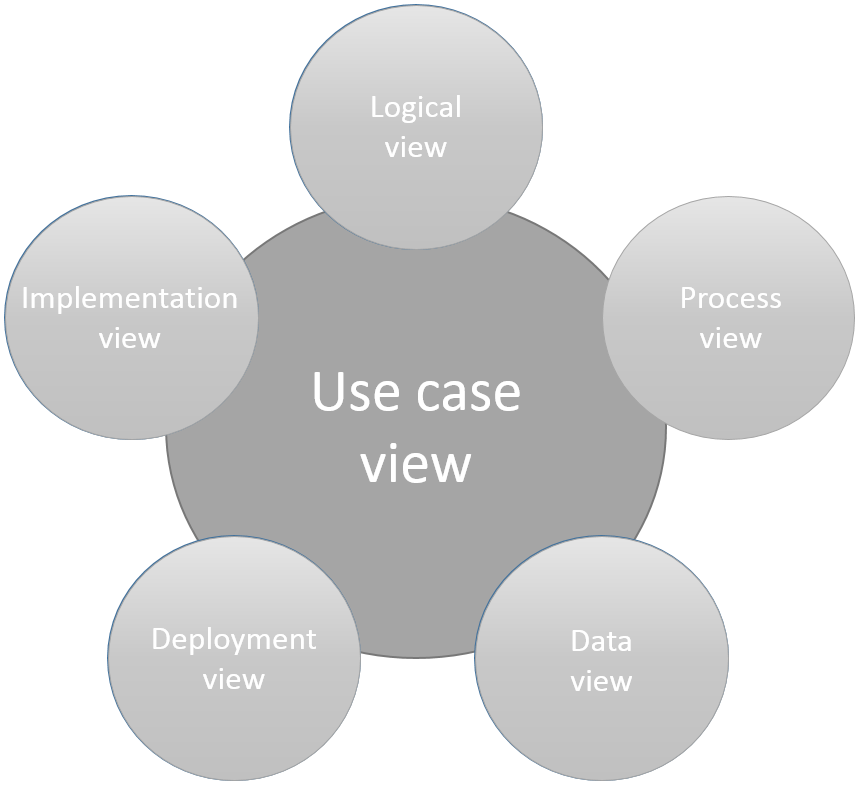
\includegraphics[width=0.7\textwidth]{Billeder/n+1}
	\vspace{0cm}
	\caption{5 + 1 view model}
	\label{fig:5 + 1 view model}
\end{figure}


\newpage

\subsection{View beskrivelser}

\textbf{Use case view}\\
Use case viewet består af use case diagrammer, som er udviklet ud fra bruges synspunkt og bruges til at beskrive systemets forskellige brugsscenarier. Alle udarbejdede use case diagrammer forefindes i kravspecifikations dokumentet.

\textbf{Logical view}\\
Logical viewet består i udgangspunkt af følgende fire diagrammer: Designoverviewdiagrammer, sekvensdiagrammer, statemachines og klassediagrammer. Først laves designoverviewdiagrammer, dernæst udarbejdes sekvensdiagrammer som bruges til at beskrive det overordnede flow i systemet. Hvis det giver mening udarbejdes statemachines, som bruges til at vise hvilke states en given use case indeholder. Til sidst laves klassediagrammer og alle "aktive" klasser identificeres. 

\textbf{Process view}\\
Process viewet beskriver de forskellige processer/tråde i systemet og hvordan samspillet imellem disse er. Primært beskrives sammenspil mellem processer/tråde der kører sideløbende med hinanden.

\textbf{Data view}\\
I data viewet beskrives layout af data der gemmes og hvordan det lagres. Desuden beskrives hvordan data bevæger sig rundt i systemet og hvordan database tilgås. 

\textbf{Deployment view}\\
I deployment viewet kigges på systemets mest grundlæggende og overordnede klasser. Det beskrives hvilke forskellige softwareklasser der bruges i hver af de grundlæggende klasser. Desuden beskrives hvilke protokoller der er anvendt i systemet, fx. layout af meddelelser med header/start/stop.   

\textbf{Implementation view}\\
I løbet af et længere projekt forløb genereres altid en masse filer - i implementations viewet vises bla. hvilke filer systemet er bygget af, filstruktur og hvilken compiler der er benyttet. 
Målet med implemantations viewet er at gøre det muligt for udefrakommende at genoptage arbejde på projektet på et hvilket som helst tidspunkt.




\newpage
\section{Logical view}
\vspace{-0.4cm}
Logical view'et er udarbejdet efter de 4 iterationer defineret i kravspecifikationen. Den første iteration dækker systemets grundfunktionalitet, mens de øvrige iterationer bruges til at tilføje funktionalitet til systemet. 
I logical view'et vil der forekomme diagrammer som er gråskraveret. De elementer der er gråskraverede er udarbejdet i tidligere iteration. Iteration 1 og 2 er designet og implementeret, mens iteration 3 og 4 kun er designet.
  
Som beskrevet består logical viewet af designoverview, pakke-, sekvens-, klasse- og state machine diagrammer. Fælles for alle diagrammerne er, at de udformes ved brug af applikationsmodellen.

\subsection{Applikationsmodel}
\vspace{-0.4cm}
Applikationsmodellen tager udgangspunkt i use cases beskrevet i kravspecifikationen og domain modellen, se figur \ref{fig:domain_model}. Domain modellen bruges til at identificere softwarepakke og deres tilhørende klasser. Desginoverview og sekvensdiagrammer fortæller og viser hvordan de forskellige klasser kommunikerer, og state machines bruges til at vise systemflow.


%\subsection{Iteration \#1}
\vspace{-0.4cm}
I iteration 1 arbejdes der med blokke som dækker over systemets mest grundlæggende funktionalitet. Batteri, ESC’er, motorer og sensorer tilsluttes dronen, og dronen gøres desuden i stand til oprette forbindelse til webapplikationen via 3G-shield’et.
Server opsættes, så at basal kommunikation mellem dronen og server er muligt. Det skal bla. være muligt for dronen at uploade sin nuværende position til server. For flere detaljer vedrørende opsætning og funktionalitet af server henvises til data view'et. 
Hvordan systemet er tiltænkt at bruges beskrives i user story nedenfor:

\subsubsection*{User story}
\vspace{-0.4cm}
Bruger tænder dronen ved at tilslutte batteri. Main controller samt 3G/GPS module initialiseres og nuværende GPS position opdateres. Herefter opretter dronen forbindelse til webapplikation og sender information om sin nuværende GPS position. Fra webapplikationen er det muligt for bruger løbende at observere hvorvidt dronen er online og på hvilken GPS position dronen sidst har befundet sig.

%kommentar
\begin{figure}[H]
	\centering
	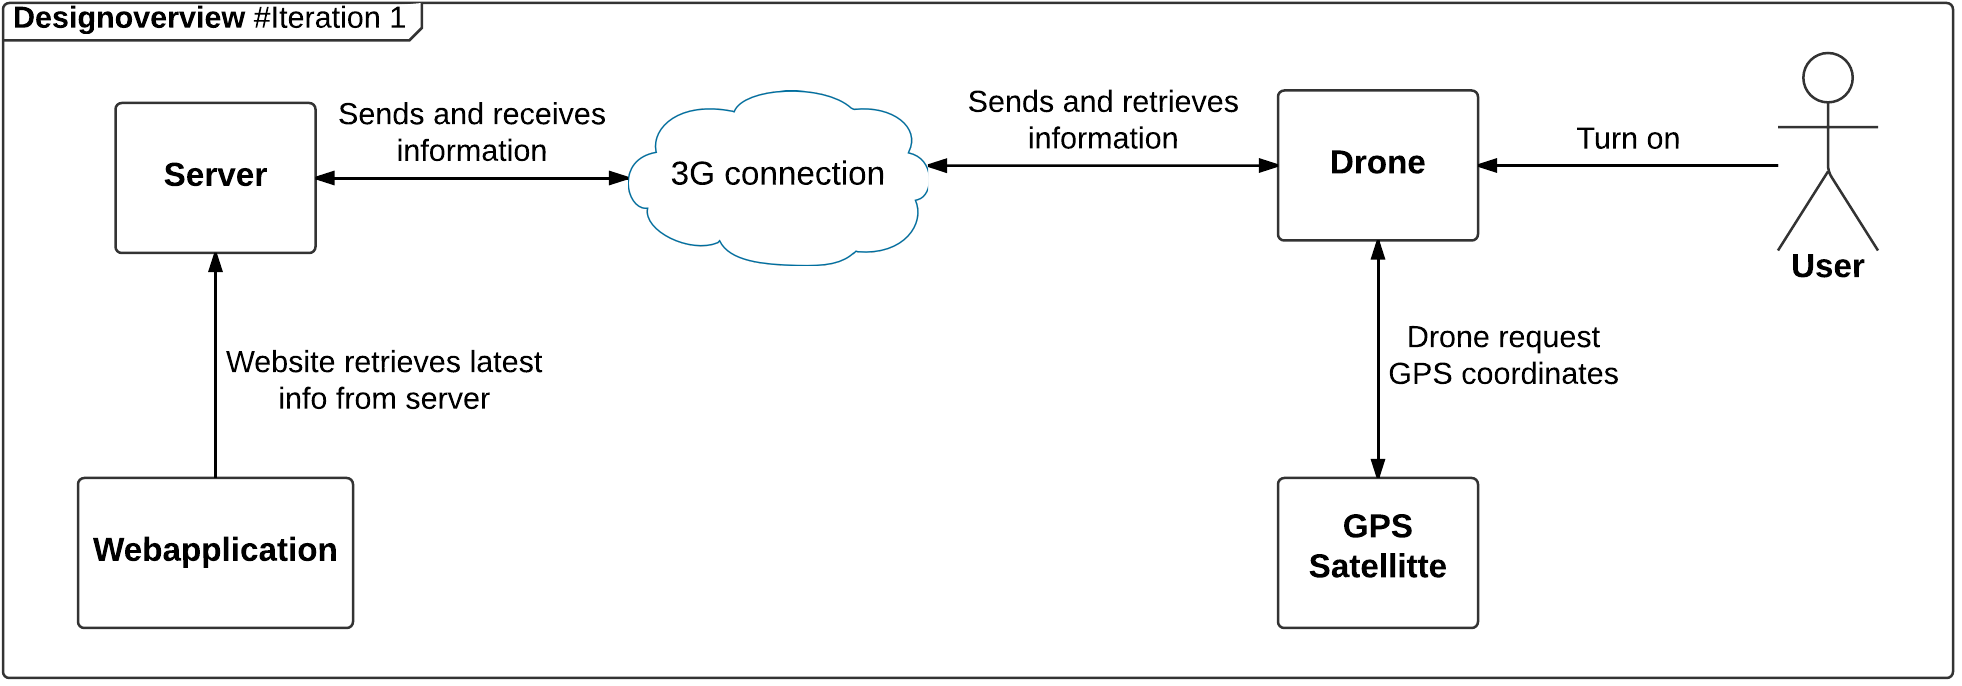
\includegraphics[width=1\textwidth]{Billeder/design_overview/design_overview_iteration1.png}
	\vspace{-.5cm}
	\caption{Design overview \#iteration 1}
	\label{fig:design_overview_UC1}
\end{figure}


\newpage
\subsubsection*{Pakkediagram drone}

I dette afsnit vises pakkediagram tilhørende drone. De pakker der vises i pakkediagrammet består af en eller flere klasser, der med stort samspil udfører opgaver indenfor et fælles ansvarsområde. På hver pakke findes en lille beskrivelse, der tydeliggør pakkens ansvarsområde. 


\begin{figure}[H]
	\centering
	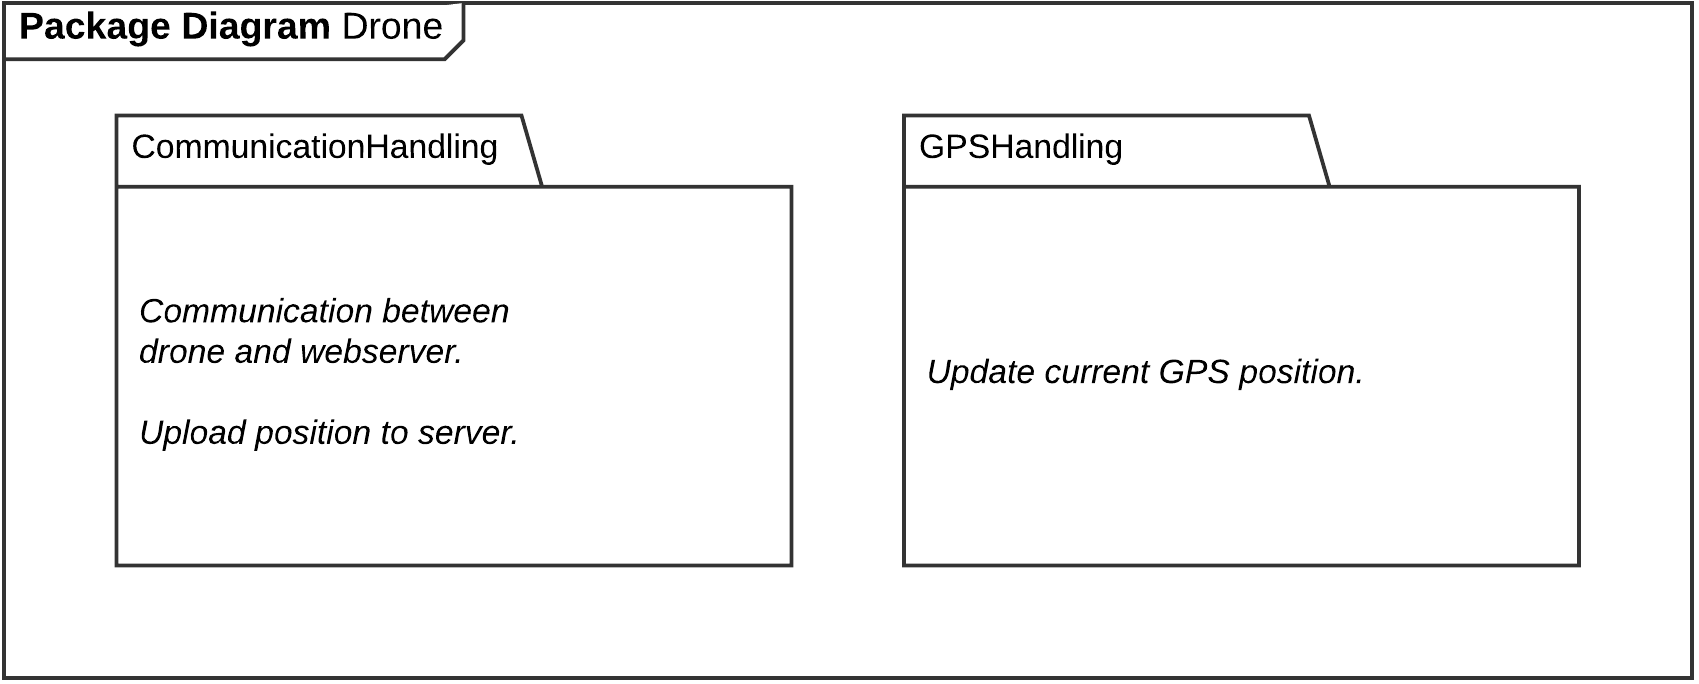
\includegraphics[width=1\textwidth]{Billeder/pakke_diagrammer/iteration1_drone.png}
	\vspace{-0.5cm}
	\caption{Pakkediagram drone}
	\label{fig:iteration1_pakke_diagram_drone}
\end{figure}

\textbf{CommunicationHandling}\\
Pakkens ansvar er kommunikation imellem drone og server. I denne iteration er der fokus på, at dronen skal kunne sende sin nuværende GPS position til server.

\textbf{GPSHandling}\\
Pakkens ansvar er håndtering af GPS. Dels er pakken ansvarlig for opstart og initiering af GPS, og desuden bruges pakken hver gang dronens nuværende GPS position skal opdateres.

\newpage
\subsubsection*{Pakkediagram webapplikation}

I dette afsnit vises pakkediagram tilhørende webapplikationen. De pakker der vises i pakkediagrammet består af en eller flere klasser, der med stort samspil udfører opgaver indenfor et fælles ansvarsområde. På hver pakke findes en lille beskrivelse, der tydeliggør pakkens ansvarsområde. 

\begin{figure}[H]
	\centering
	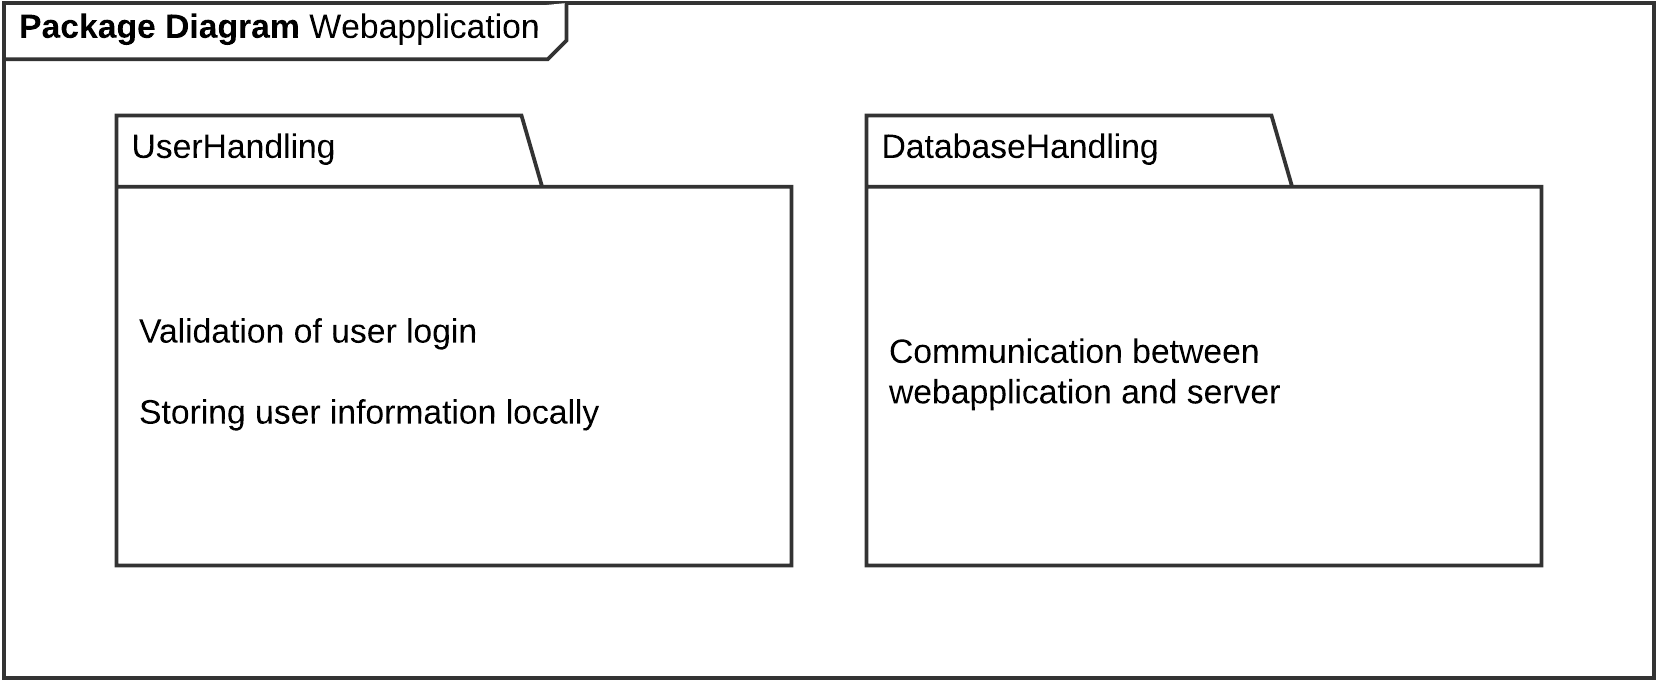
\includegraphics[width=1\textwidth]{Billeder/pakke_diagrammer/iteration1_server.png}
	\vspace{-0.5cm}
	\caption{Overordnet pakke diagram over webapplikationen}
	\label{fig:iteration1_pakke_diagram_webapp}
\end{figure}

\textbf{UserHandling}\\
Pakkens ansvar er validering af login/log ud på websitet. Pakken har også ansvaret for at hente og gemme data om den pågældende bruger.

\textbf{DatabaseHandling}\\
Pakkens ansvar er kommunikation imellem databasen og serveren. 


\newpage
\subsubsection*{Sekvensdiagram drone}
På sekvensdiagrammet på figur \ref{fig:Sekvens_diagram_iteration1}, vises hvilke klasser der indgår og bruges i første iteration. Af sekvensdiagrammet fremgår det, at sekvensen først startes når bruger tilslutter batteri og tænder dronen. Når der er tilkoblet forsyning initialiseres main controller samt 3G/GPS og nuværende GPS position  (longitude og latitude) opdateres. Dronens nuværende GPS position opdateres når dronen sender PUT requests til websitet. PUT requests bruges dels til at fortælle websitet at dronen er online og dels til at give websitet information om dronens nuværende position. 

%kommentar
\begin{figure}[H]
	\centering
	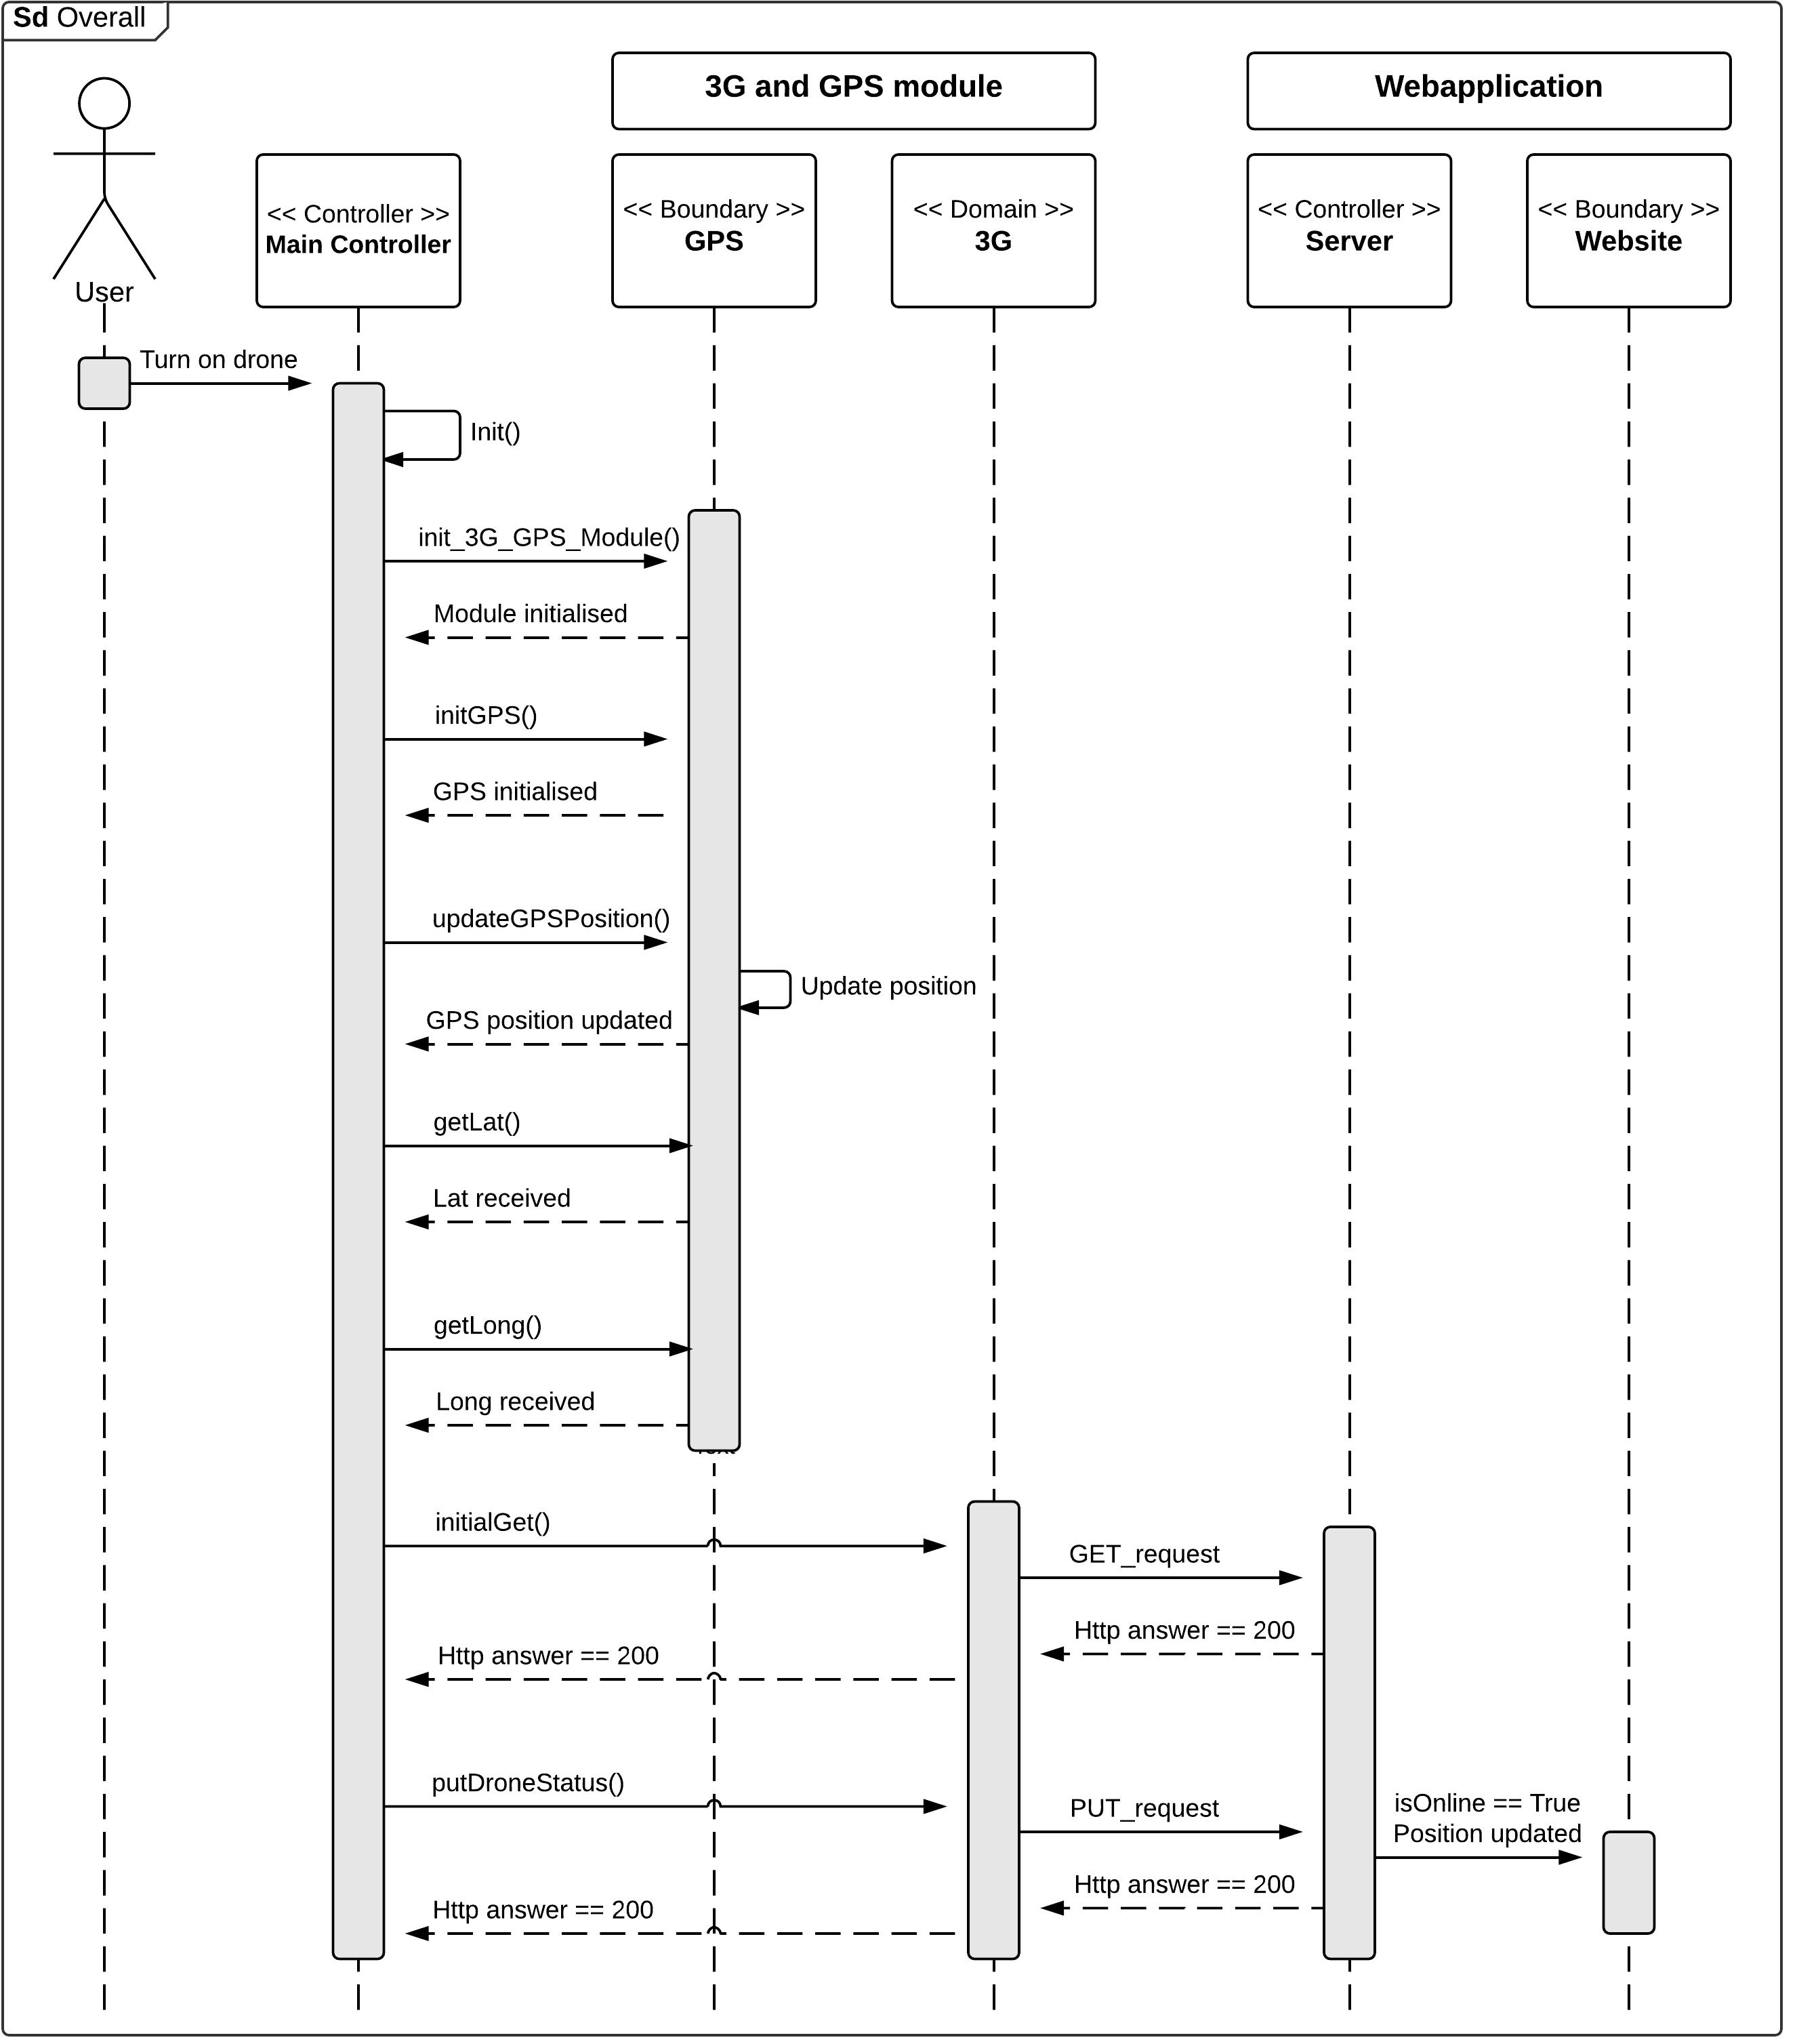
\includegraphics[width=1\textwidth]{Billeder/sekvens/sekvens_iteration1}
	\caption{Sekvens diagram \#iteration 1}
	\label{fig:Sekvens_diagram_iteration1}
\end{figure}
\newpage

På figur \ref{fig:Sekvens_diagram_initialget} og figur \ref{fig:Sekvens_diagram_putDroneStatus} bliver 3G modulet yderligere uddybet.\\
\ref{fig:Sekvens_diagram_initialget} viser hvilke klasser der anvendes til at hente data fra serveren. 

\begin{figure}[H]
	\centering
	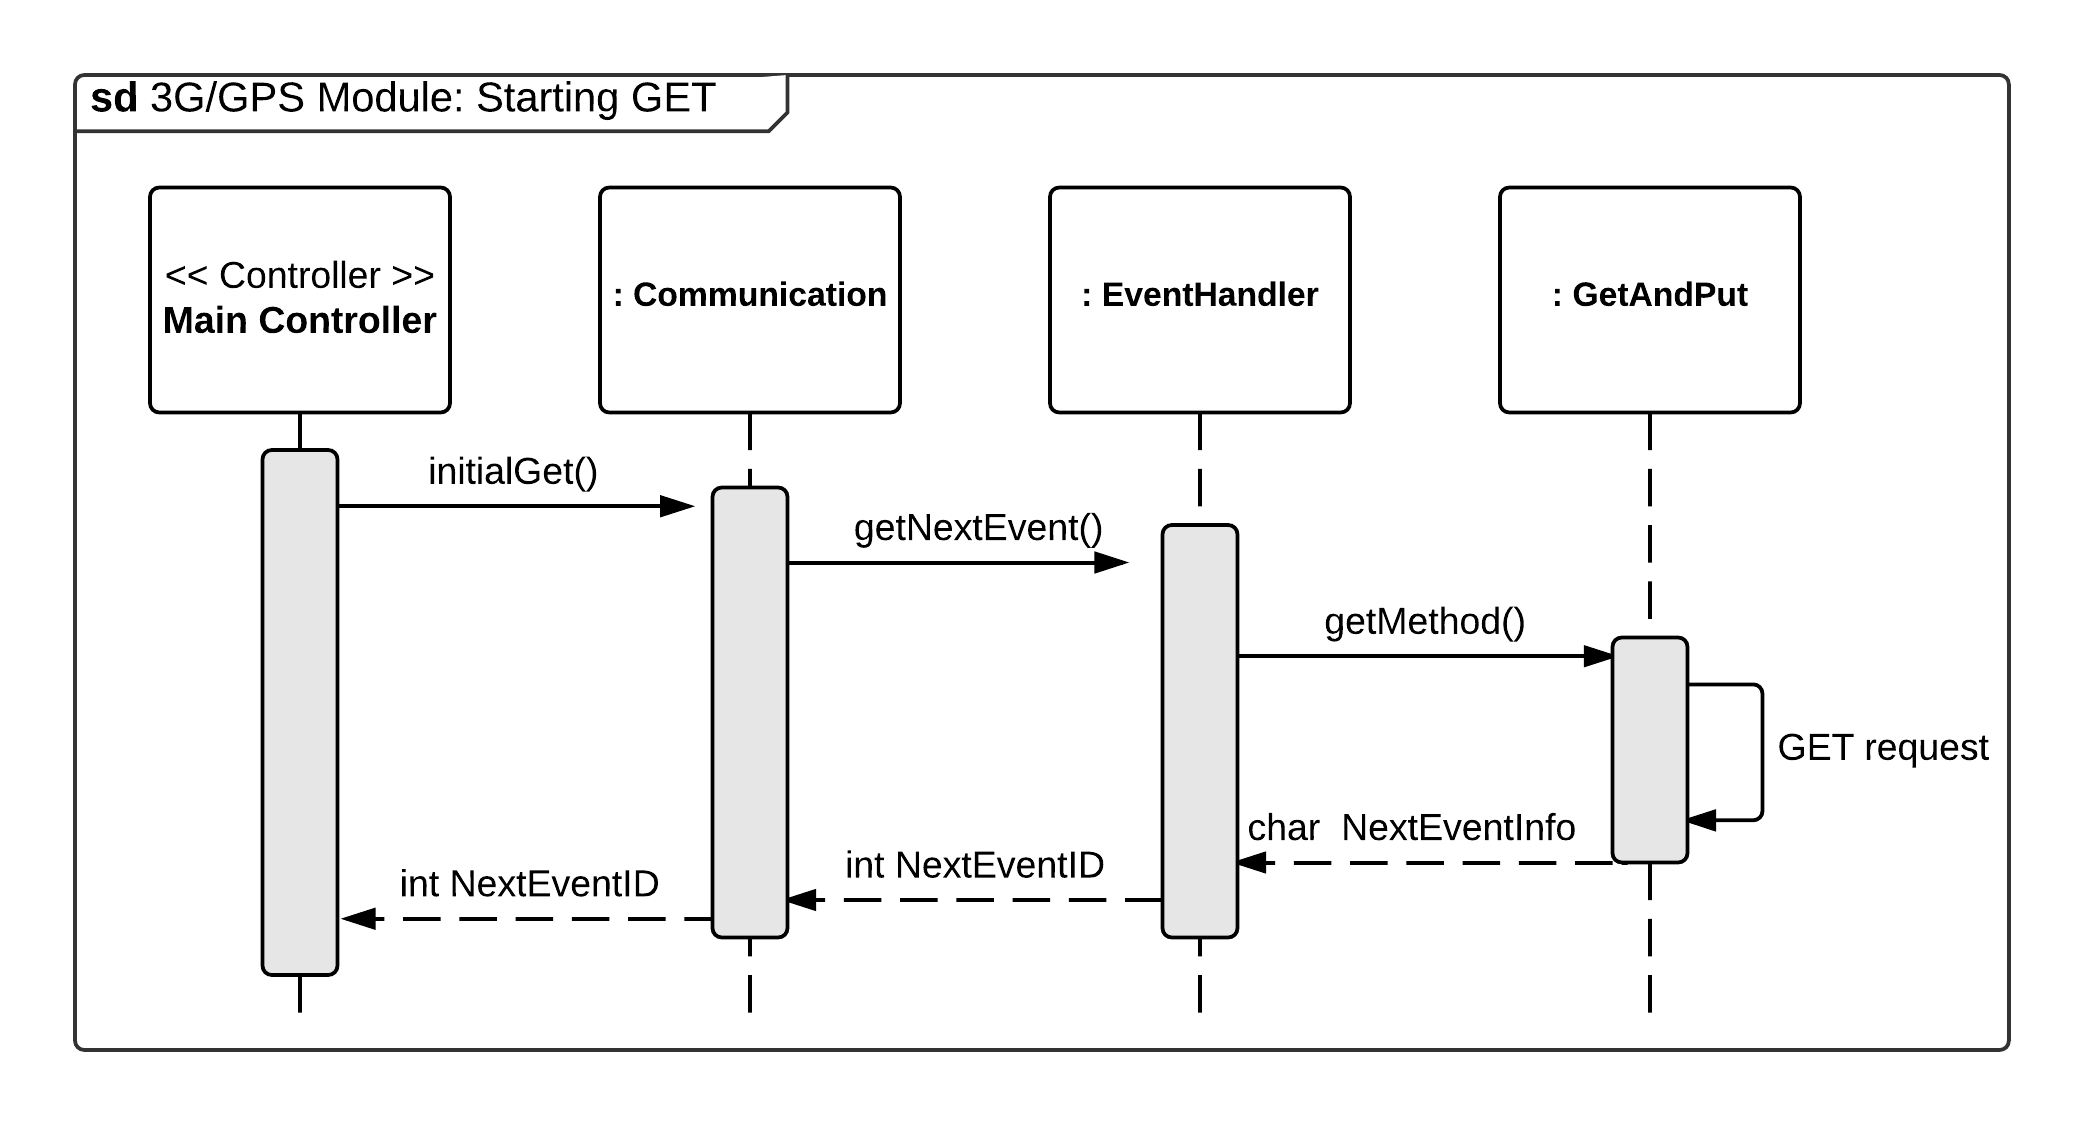
\includegraphics[width=1\textwidth]{Billeder/sekvens/sekvens_iteration1_initialget}
	\caption{Sekvens diagram \#iteration 1 - initialget}
	\label{fig:Sekvens_diagram_initialget}
\end{figure}

\vspace{.5cm}

De data der hentes med GET requestet, bruges sammen med PUT requestet. For at kunne udføre et PUT request, skal data der ønskes sendt til server stemme overens med det data der i forvejen ligger på serveren.

\begin{figure}[H]
	\centering
	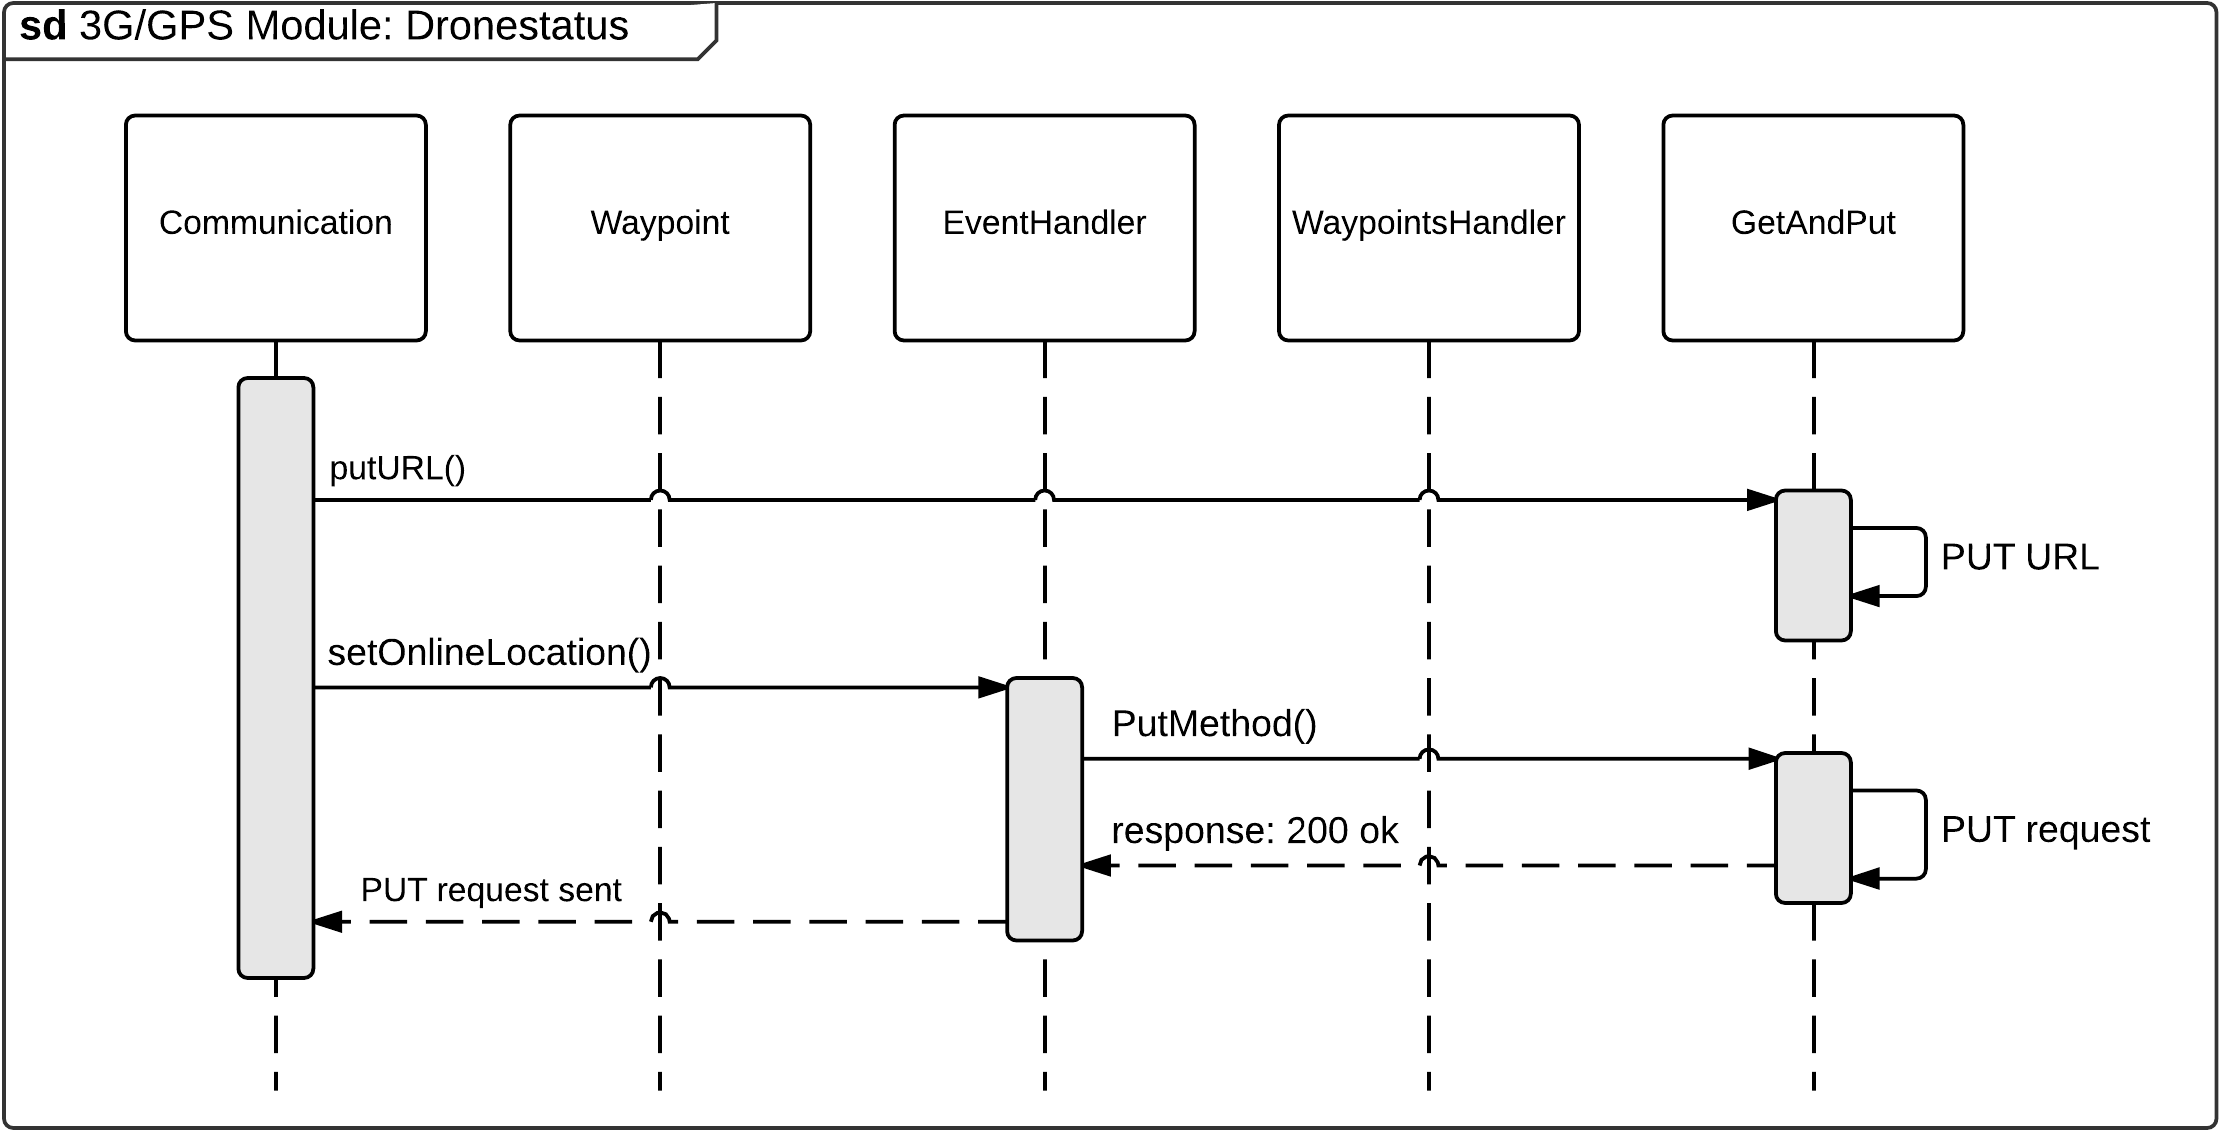
\includegraphics[width=1\textwidth]{Billeder/sekvens/sekvens_iteration1_putdronestatus}
	\caption{Sekvens diagram \#iteration 1 - putDroneStatus}
	\label{fig:Sekvens_diagram_putDroneStatus}
\end{figure}


\newpage

\subsubsection*{Sekvensdiagram webapplikation}
På figur \ref{fig:Sekvens_diagram_login} ses sekvens diagrammet over login på webappplikationen. På diagrammet vises det at useren først bliver ført til næste side ved succesfuld login. Diagrammet viser også kommunikationen med CRUDServiceDrone som kommunikerer med databasen. Diagrammet viser også hvordan AuthenticationServices setter den givet users data inden useren bliver ført vider i systemet.

\begin{figure}[H]
	\centering
	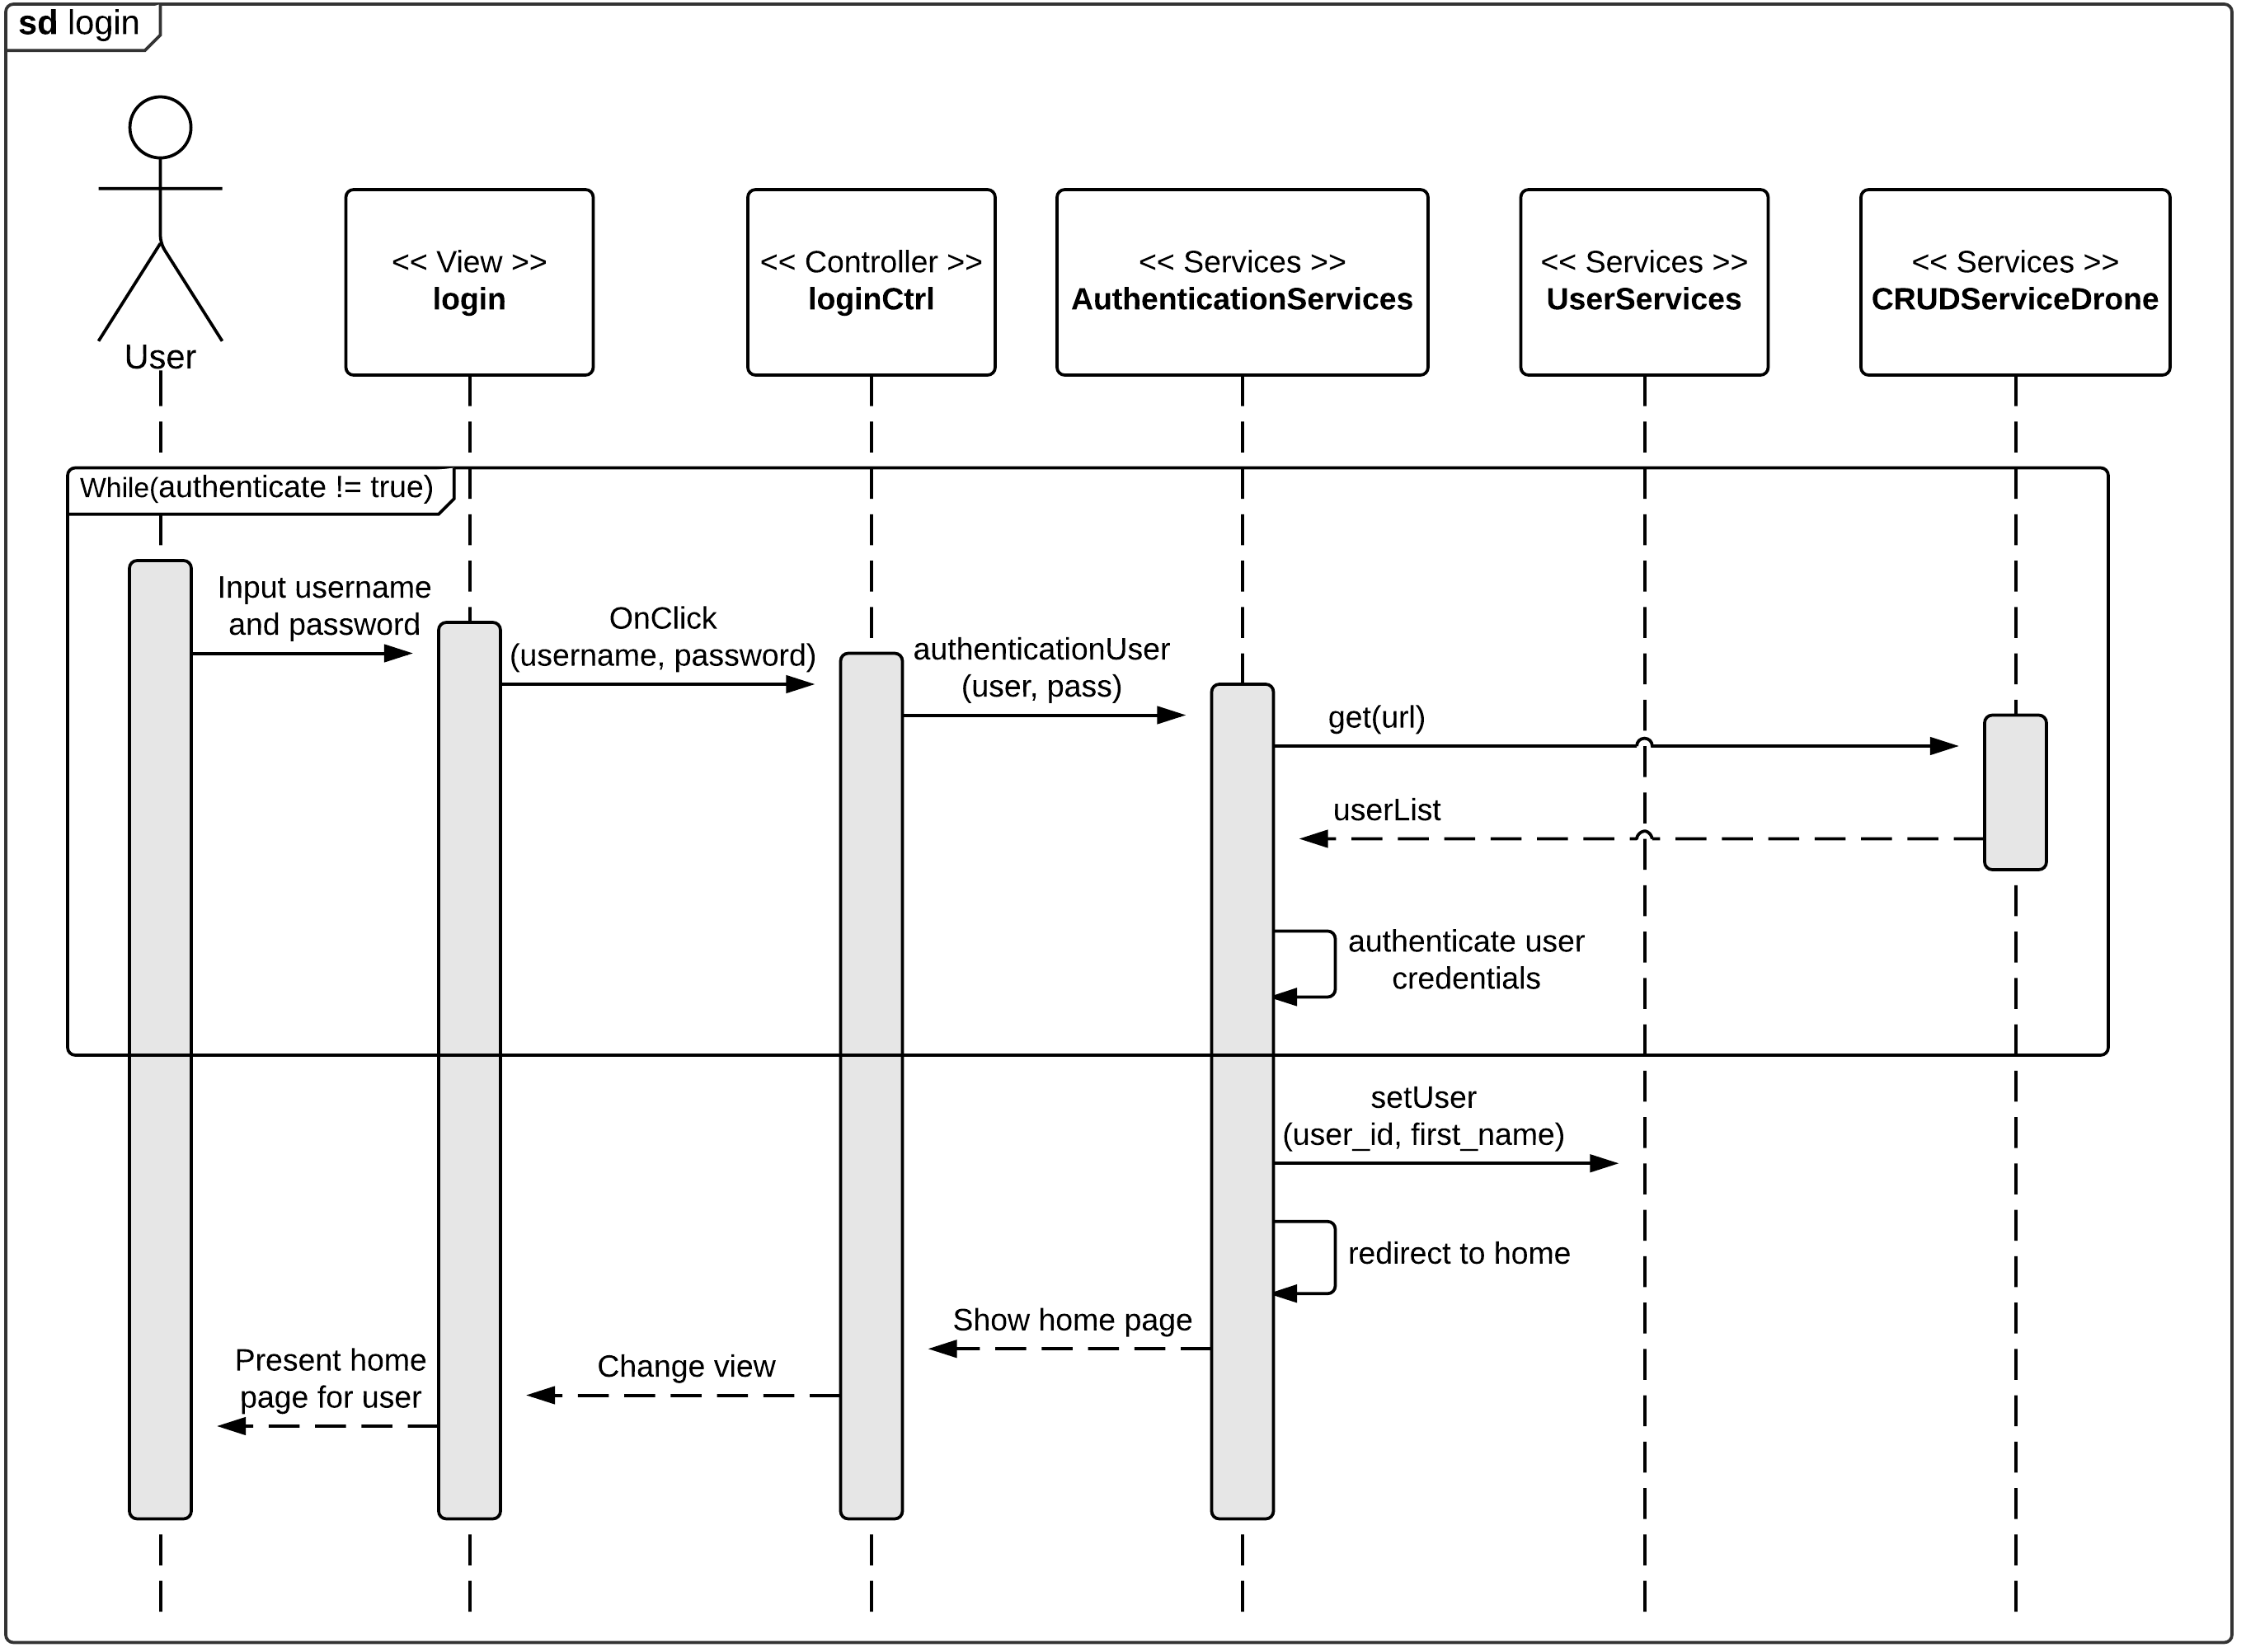
\includegraphics[width=1\textwidth]{Billeder/sekvens/login_sq_diagram.png}
	\caption{Sekvens diagram login}
	\label{fig:Sekvens_diagram_login}
\end{figure}
\newpage


\subsubsection*{Klassediagram drone}
\vspace{-0.2cm}
Figur \ref{fig:classDiagram_iteration1} vises et klassediagram tilhørende iteration 1. Klassediagrammet viser iterationens vigtigste klasser, samt deres tilhørende metoder og attributter. På den følgende side forefindes en kort beskrivelse klasserne og deres metoder.

\vspace{-0.2cm}
%kommentar
\begin{figure}[H]
	\centering
	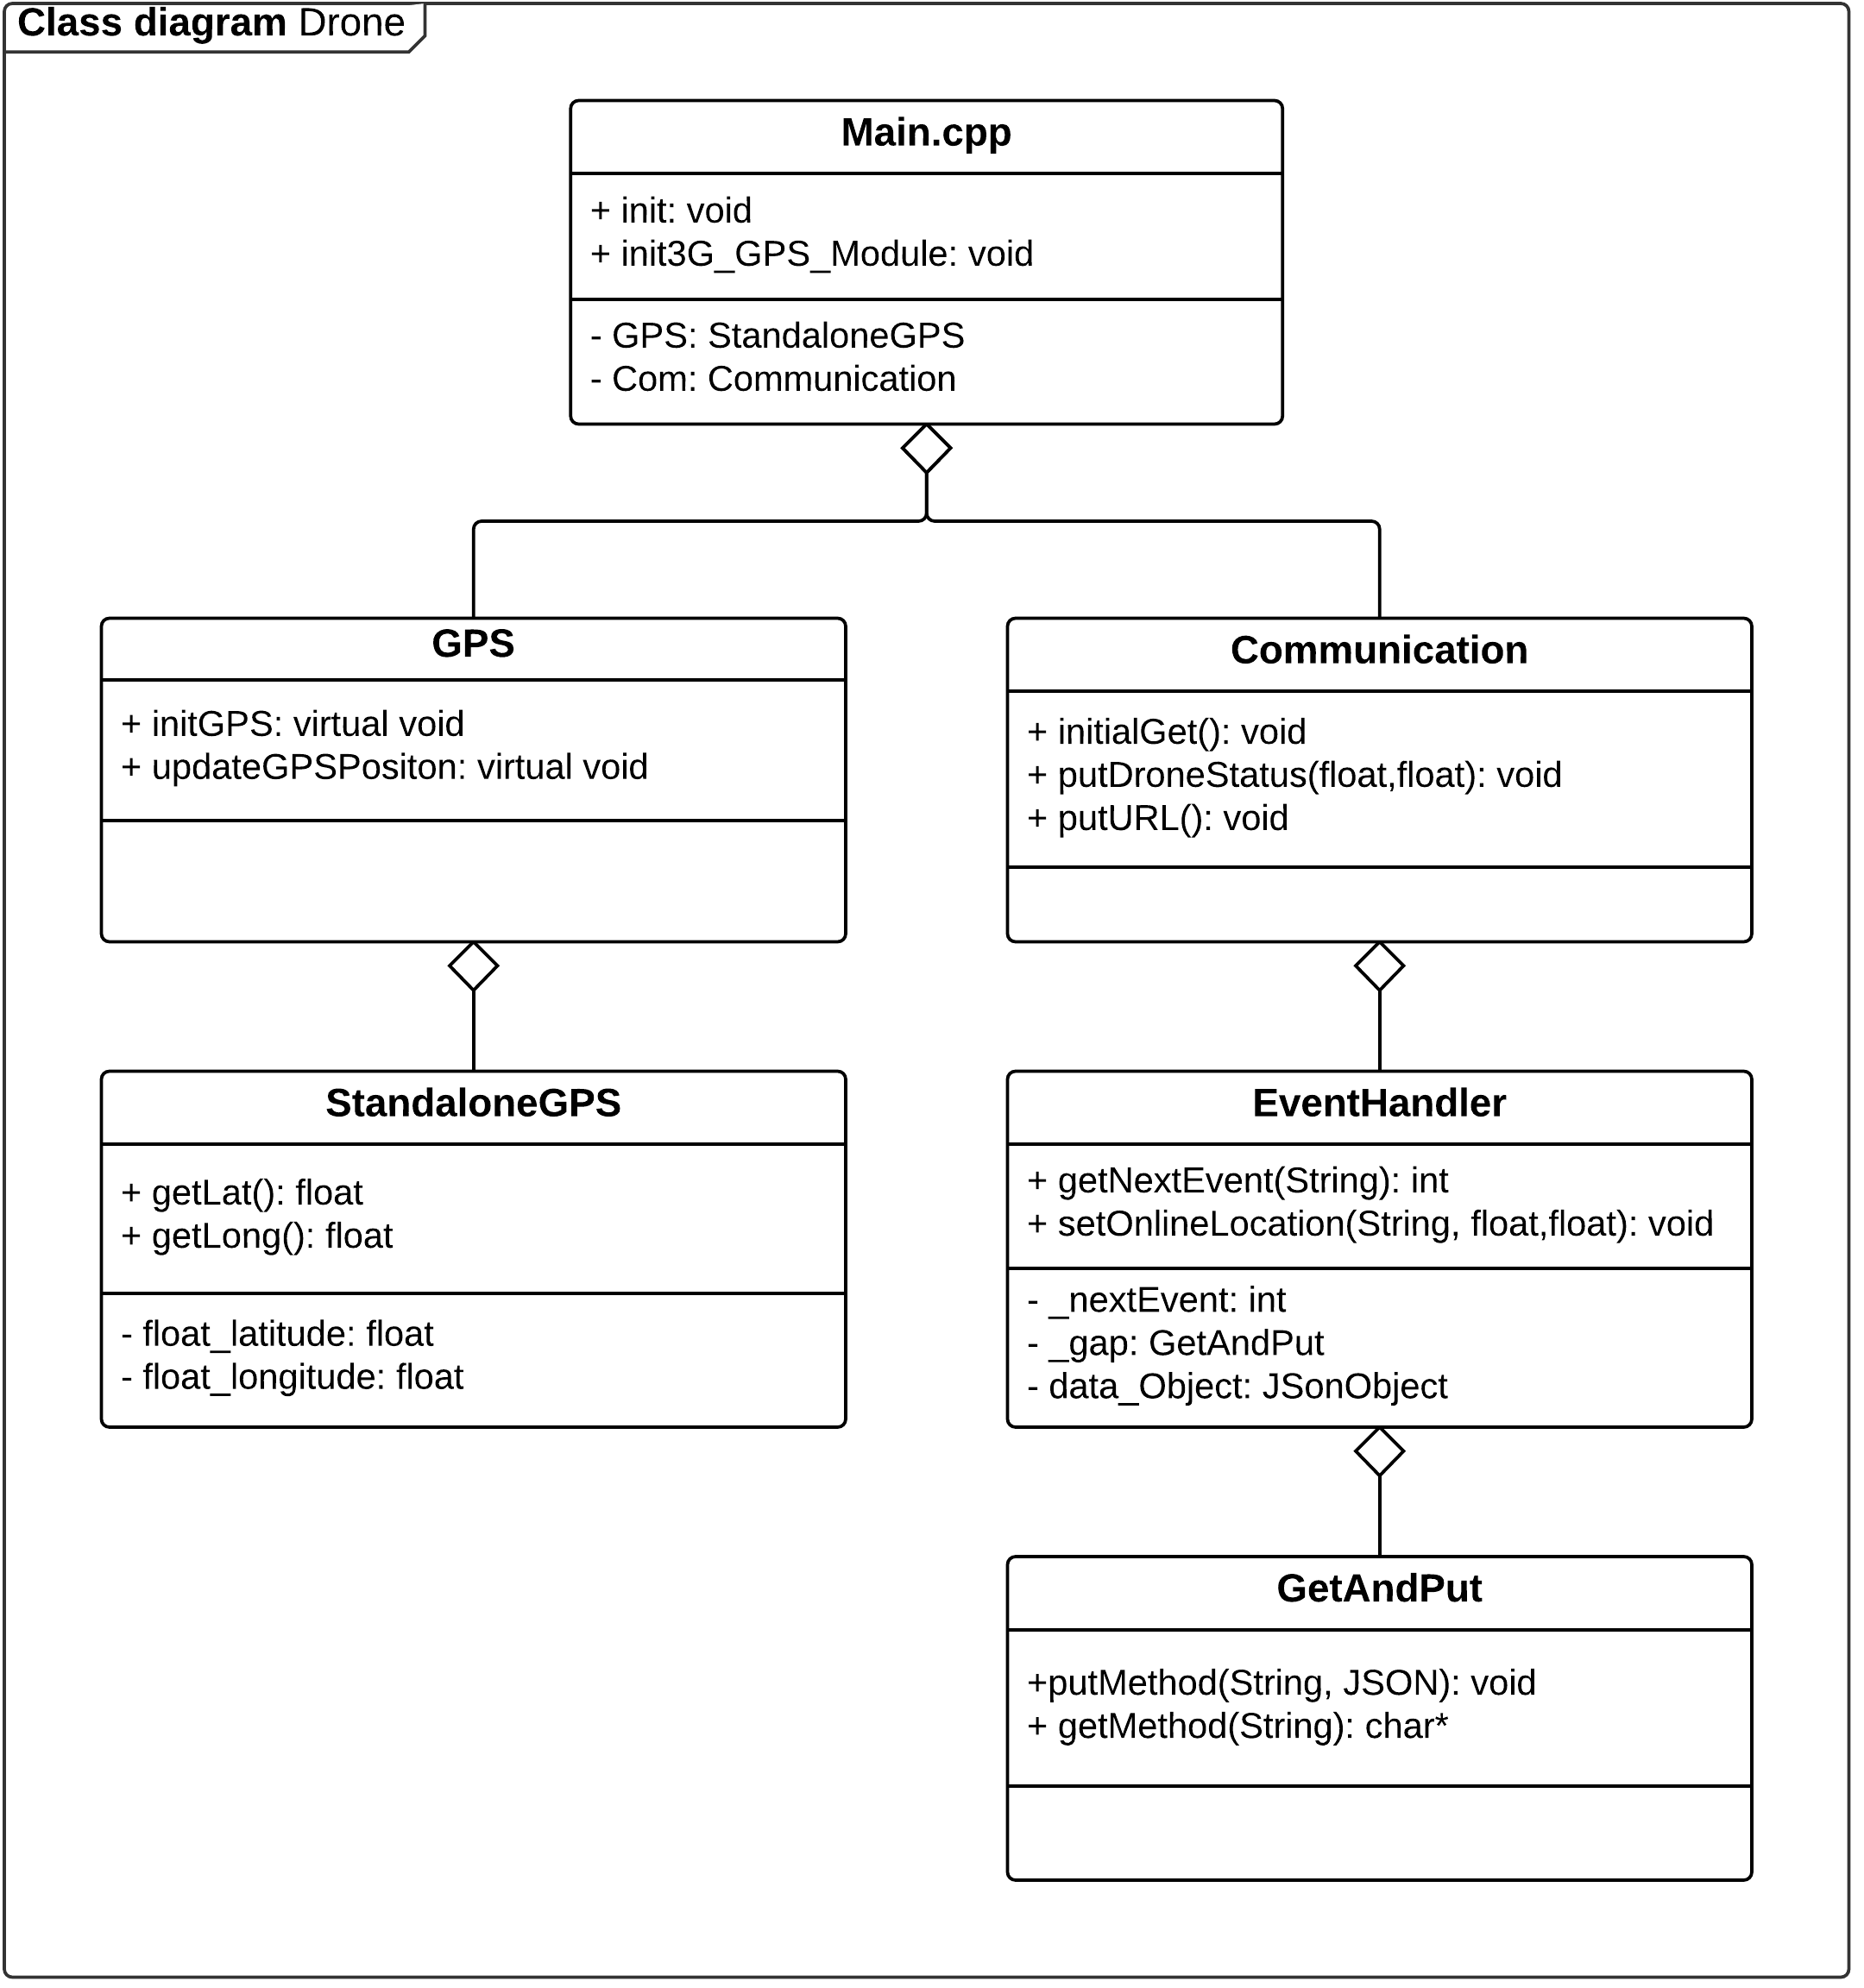
\includegraphics[width=1\textwidth]{Billeder/klasse_diagrammer/classdiagram_iteration1.png}
	\vspace{-0.5cm}
	\caption{Klassediagram \#iteration 1}
	\label{fig:classDiagram_iteration1}
\end{figure}
\vspace{-0.1cm}

\textbf{Main.cpp} \\
Main.cpp filen bruges til at sætte arduino board korrekt op, bla. sættes baudrate på de forskellige serielle forbindelser. Desuden bruges Main.cpp til at kalde og eksekverer forskellige klasse, objekter og funktioner.

\textbf{GPS} \\
GPS klassen er implementeret som en abstract klasse, idet den ikke selv har nogle metoder den skal bruge, men med virtuelle metoder der sikrer at de implementeres i de afledte klasser. 
Init og updateGPSPosition er valgt til at være virtuelle klasser, hvilket gør at de skal implementeres uanset hvilken GPS der bruges. Klassen er lavet fordi der i udgangspunkt var mulighed for at bruge 3 forskellige slags GPS modes med 3G/GPS shieldet. 

\textbf{StandaloneGPS}\\
Denne klasse er ansvarlig for al kommunikation med GPS'en når standalone mode er valgt. 

\newpage

Nedenfor ses figur \ref{fig:udvidet3G_it1} som er en udvidet klasse diagram over 3G modulet. Klasse diagrammet viser et udvidet klasse diagram, der viser hvilke metoder der indgår i iteration 1 for 3G modulet. 

\begin{figure}[H]
	\centering
	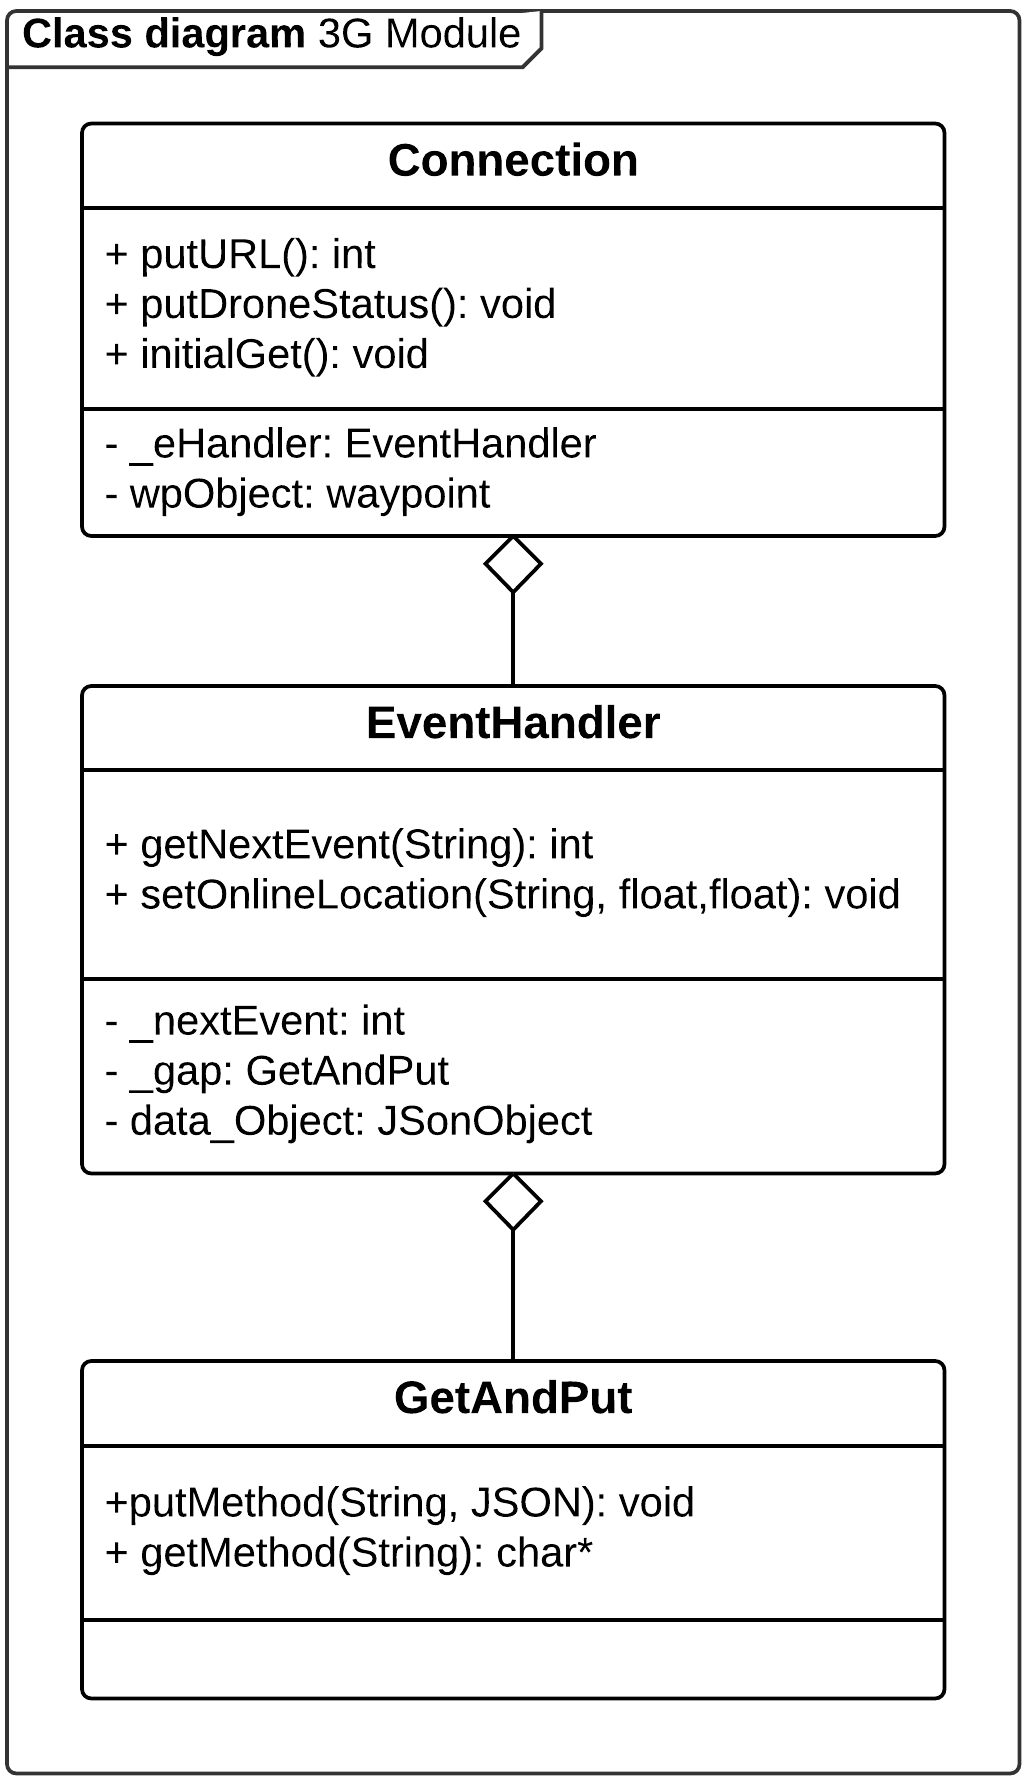
\includegraphics[width=0.50\textwidth]{Billeder/klasse_diagrammer/udvidet3G_iteration1.png}
	\vspace{0.5cm}
	\caption{Udvidet klasse diagram for 3G modulet - iteration 1}
	\label{fig:udvidet3G_it1}
\end{figure}

\textbf{GetAndPut} \\
GetAndPut klassen er den klasse der er tættest på hardwaren. Klassen indeholder de http metoder der bruges til kommunikation mellem dronen og serveren. 

\textbf{Communication} \\
Communication klassen er den øverste klasse og den håndterer sammen med andre klasser, alt der har med 3G at gøre.

\textbf{EventHandler} \\
EventHandleren er den klasse der håndterer Events. EventHandleren er bindeledet mellem communication- og GetAndPut klassen. EventHandleren sorterer eventID'et fra de data den modtager og returnerer værdien til communication klassen. 


\newpage

\subsubsection*{Klassediagram website}
\vspace{-0.2cm}
Figur \ref{fig:classDiagram_login} viser klassediagrammet tilhørende websitet for iteration 1.
\vspace{-0.2cm}
\begin{figure}[H]
	\centering
	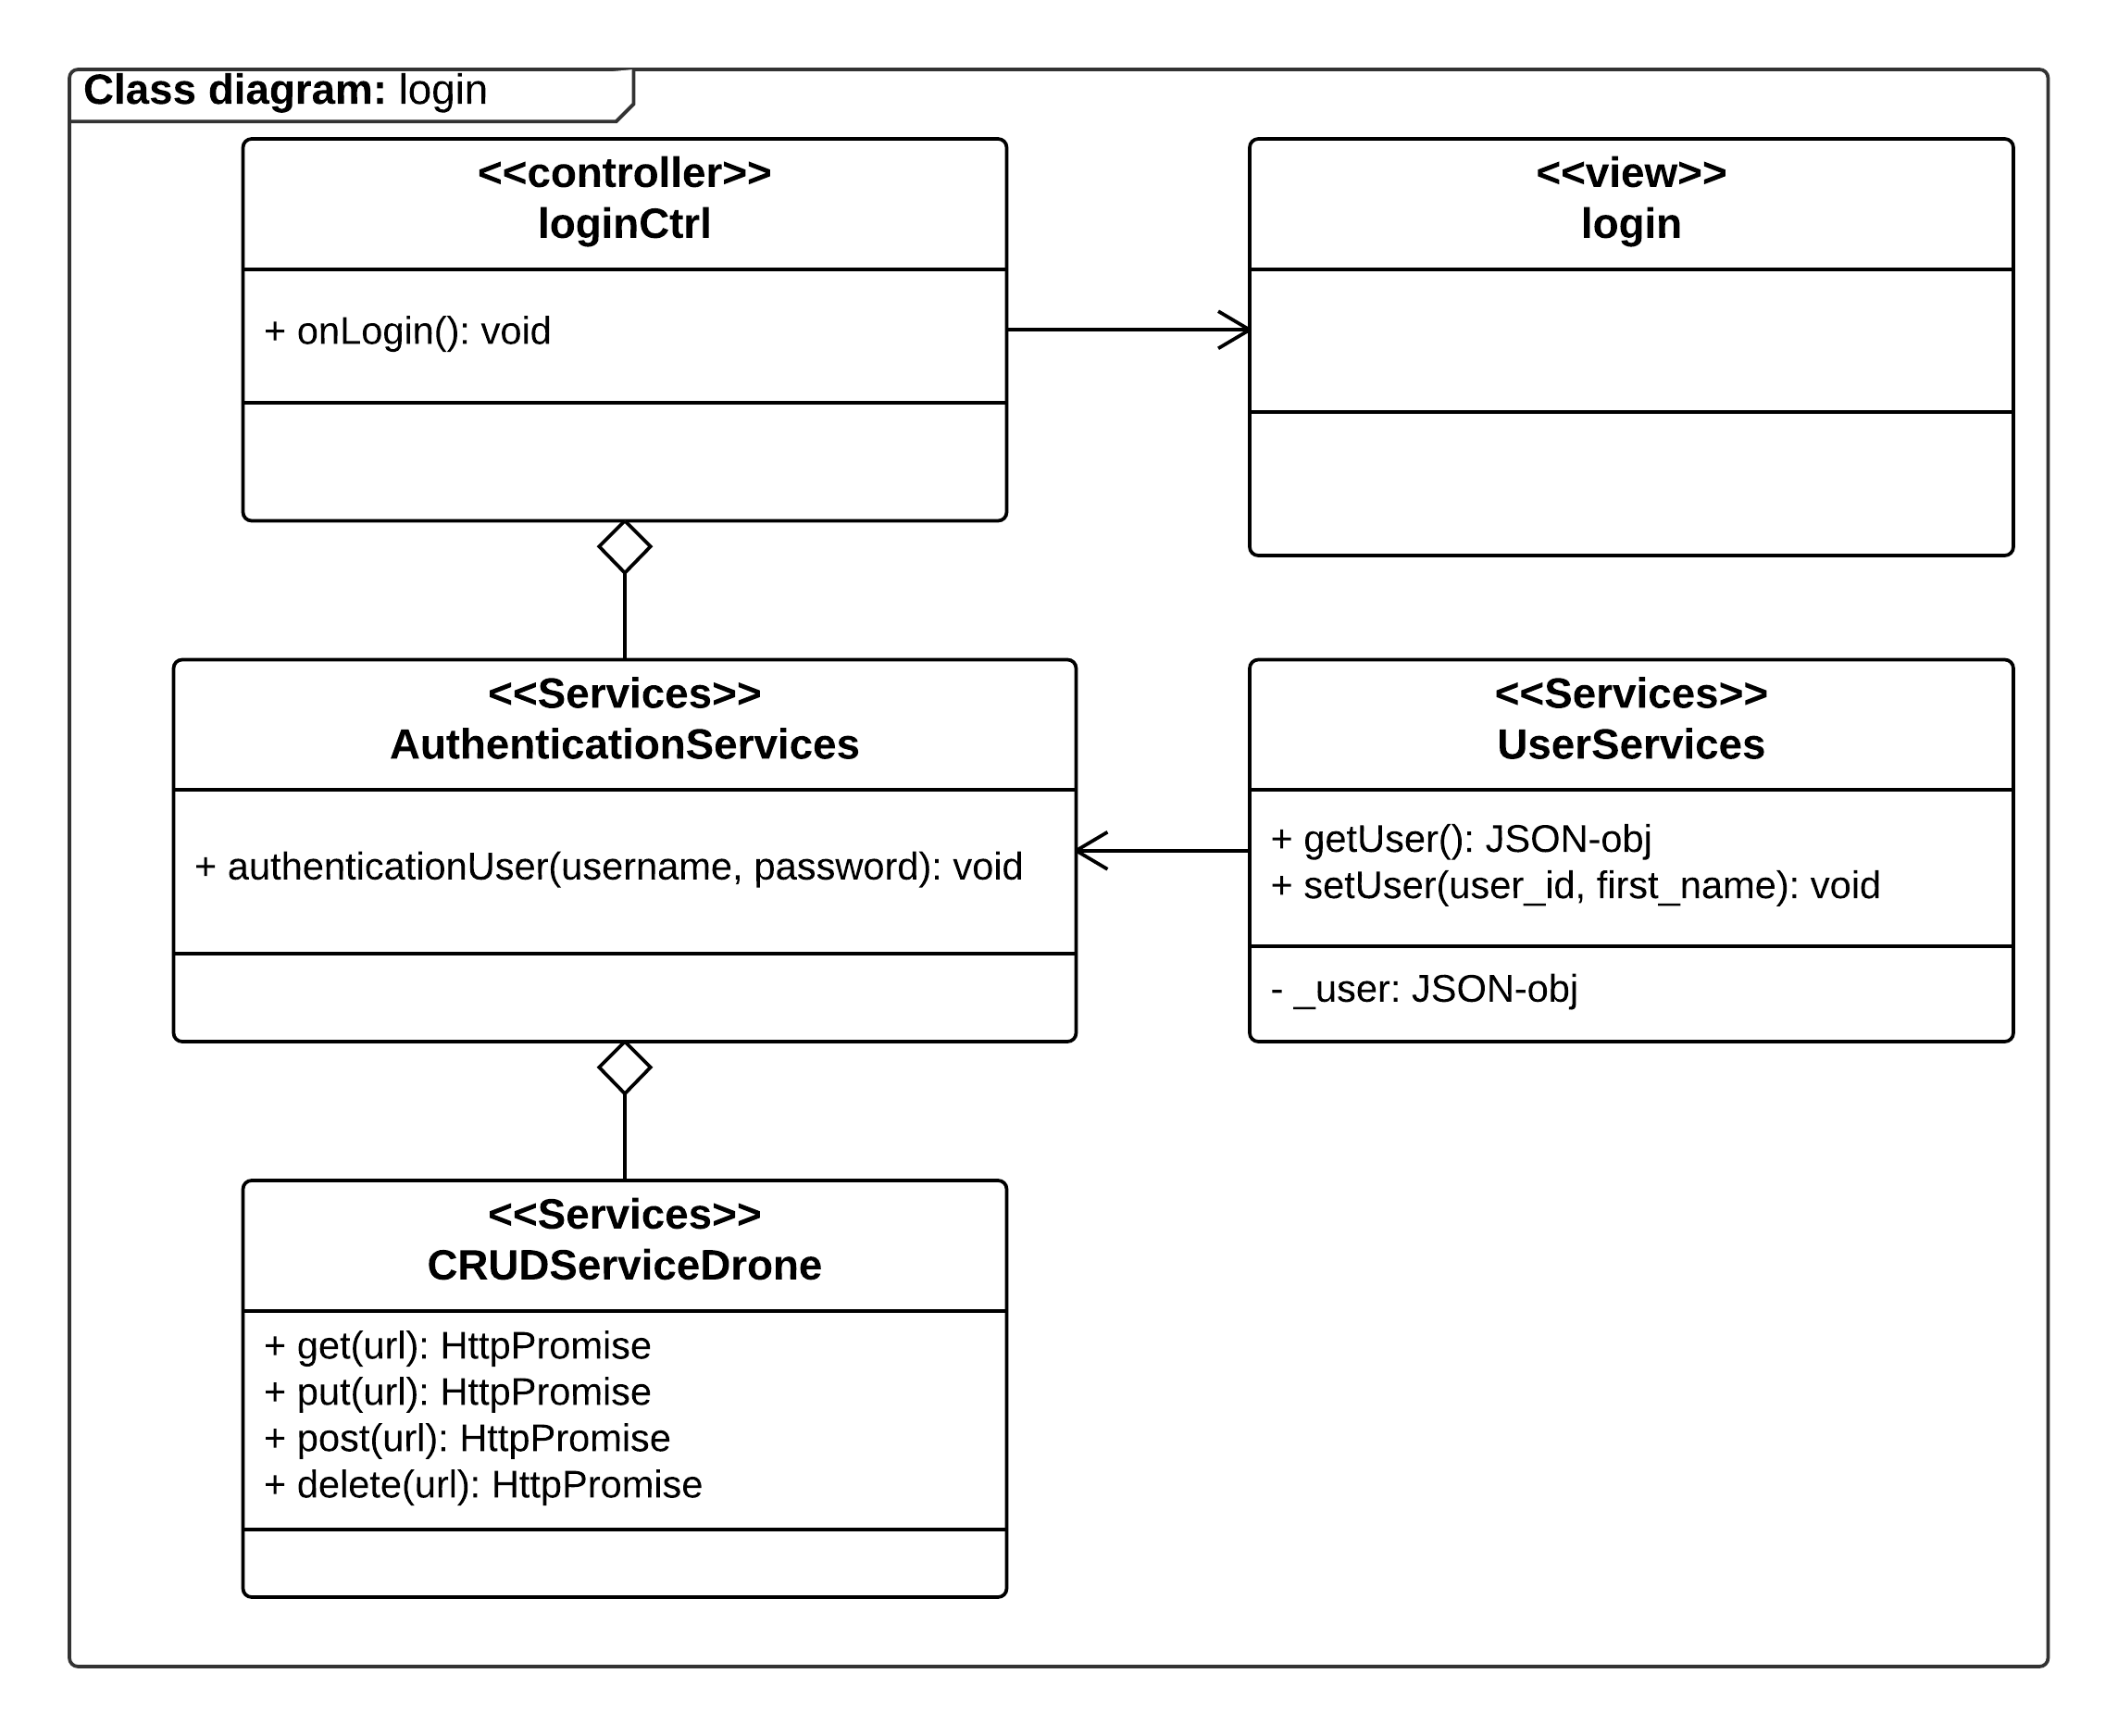
\includegraphics[width=1\textwidth]{Billeder/klasse_diagrammer/login_class_diagram.png}
	\vspace{-0.5cm}
	\caption{Klassediagram login}
	\label{fig:classDiagram_login}
\end{figure}

\vspace{-0.2cm}

\textbf{login} \\
Login view filen er det html script som useren ser på sin webclient. Filen er two-way databinded med loginCtrl klassen. Via denne binding kan der sendes og modtages data direkte.

\textbf{loginCtrl} \\
LoginCtrl er controller klassen som er forbundet med view klassen via two-way databinding. Klassen uddelegere også opgaver til dens services.

\textbf{AuthenticationServices} \\
AuthenticationServices er en service der afgør om user er authenticated eller ej. Hvis user er authenticated bliver han redirected til websitets home-page. Klassen gør brug af UserServices til at gemme information om den user der er logget ind i systemet.

\textbf{UserServices}\\
UserServices indeholder information om user der er logget ind i systemet.

\textbf{CRUDServiceDrone} \\
CRUDServiceDrone er den service der styre alt kontakt til databasen i systemet. Igennem denne service er det muligt at hente, opdater og poste data til databasen.


\subsubsection*{State machine diagram}
\vspace{-0.1cm}
I state machine diagrammet på figur \ref{fig:Statemachine_iteration1}, vises de forskellige states der eksisterer i iteration 1 og hvordan flowet imellem dem ser ud. Der eksisterer givet vis kun 2 states i iteration 1, men state machinen er medtaget fordi den på nem og overskuelig vis illustrerer systemflowet.
%kommentar
\begin{figure}[H]
	\centering
	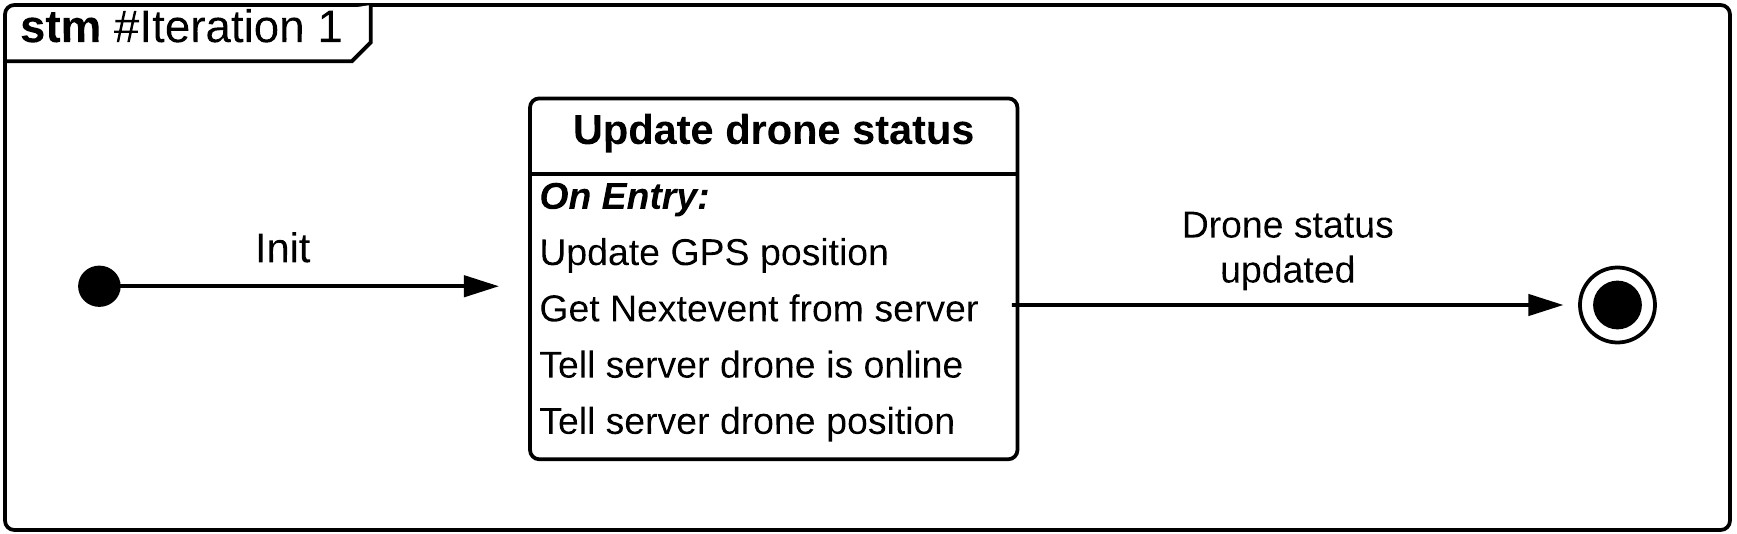
\includegraphics[width=1\textwidth]{Billeder/statemachine/State_iteration1.png}
	\vspace{-0.5cm}
	\caption{Statemachine \#iteration 1}
	\label{fig:Statemachine_iteration1}
\end{figure}

\newpage
\subsection{Iteration \#2}
I iteration 2 er formålet at færdiggøre funktionalitet på websitet så det muliggøres at oprette nye waypoints til dronen og at muliggøre autonome flyvning. Bruger skal kunne oprette flyveopsætninger og gøre dem tilgængelig for dronen, hvilket kræver yderlige kommunikations opsætning hos mellem drone. Ydermere skal dronen kunne finde egen GPS position, flyvehøjde og orientering. Ud fra viden om egen position, flyvehøjde og orientering skal dronen flyve til de lokationer som er fastsat i flyveopsætningen. 
Hvordan systemet er tiltænkt at bruges beskrives i user story nedenfor:

\subsubsection*{User story}
Bruger logger på webapplikationen med sit brugernavn og password. Når der er logget korrekt ind vises bruger sin eller sine droner på en liste. Ved at trykke på en drone vises bruger information om den pågældende drone. Informationen beståer af waypoints, om der skal tages billeder ved de forskellige waypoints samt indstilling af flyvehøjde. Brugeren klikker på en drone fra listen og derefter klikker på kortet for at oprette waypoints, i det waypoints bliver oprettet bliver et nyt event også oprettet. Brugeren giver eventet et navn og en kommentar og trykker på knappen "publish to drone".
Når en drone er tændt og færdig initialiseret fortæller den server webserveren om sin nuværende position og kontrollerer om en ny flyveopsætning er tilgængelig. Er der en ny flyveopsætning tilgængelig hentes den og dronen påbegynder flyvning.

%kommentar
\begin{figure}[H]
	\centering
	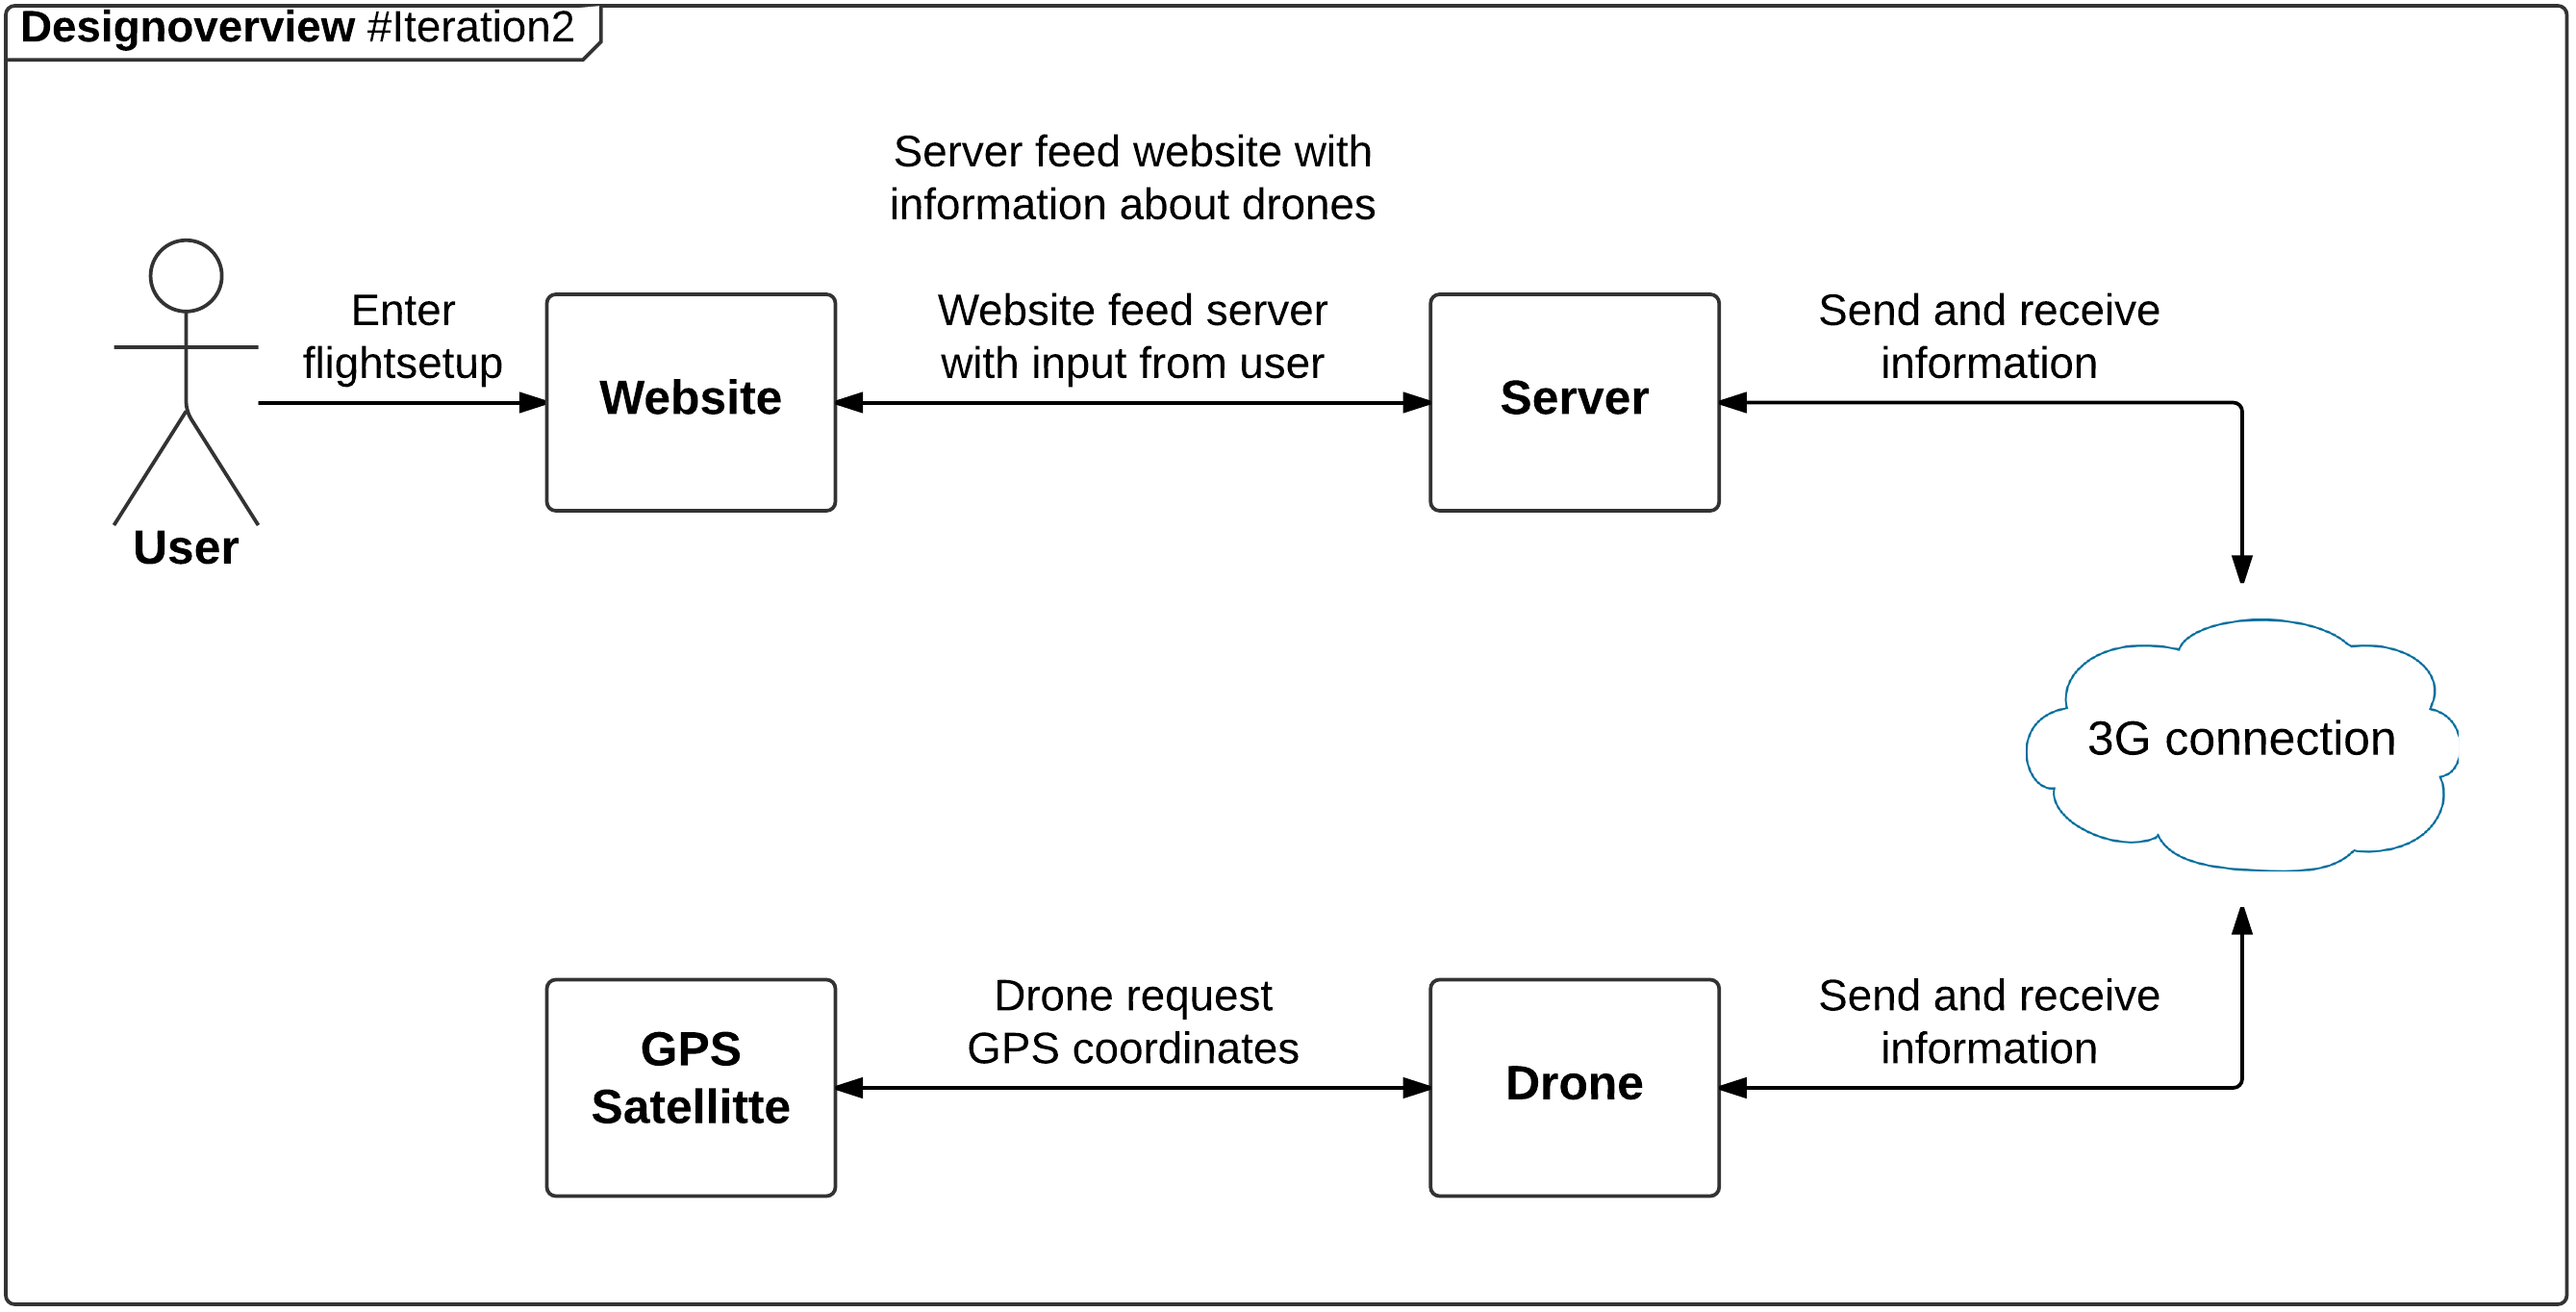
\includegraphics[width=1\textwidth]{Billeder/design_overview/design_overview_iteration2.png}
	\vspace{-.5cm}
	\caption{Designoverview \#iteration 2}
	\label{fig:design_overview_UC1}
\end{figure}


\newpage
\subsubsection*{Pakkediagram drone}
I dette afsnit vises pakkediagram tilhørende drone. De pakker der vises i pakkediagrammet består af en eller flere klasser, der med stort samspil udfører opgaver indenfor et fælles ansvarsområde. På hver pakke findes en lille beskrivelse, der tydeliggør pakkens ansvarsområde. De dele af pakkerne der er gråskraveret, er funktionalitet udarbejdet i tidligere iteration.


\begin{figure}[H]
	\centering
	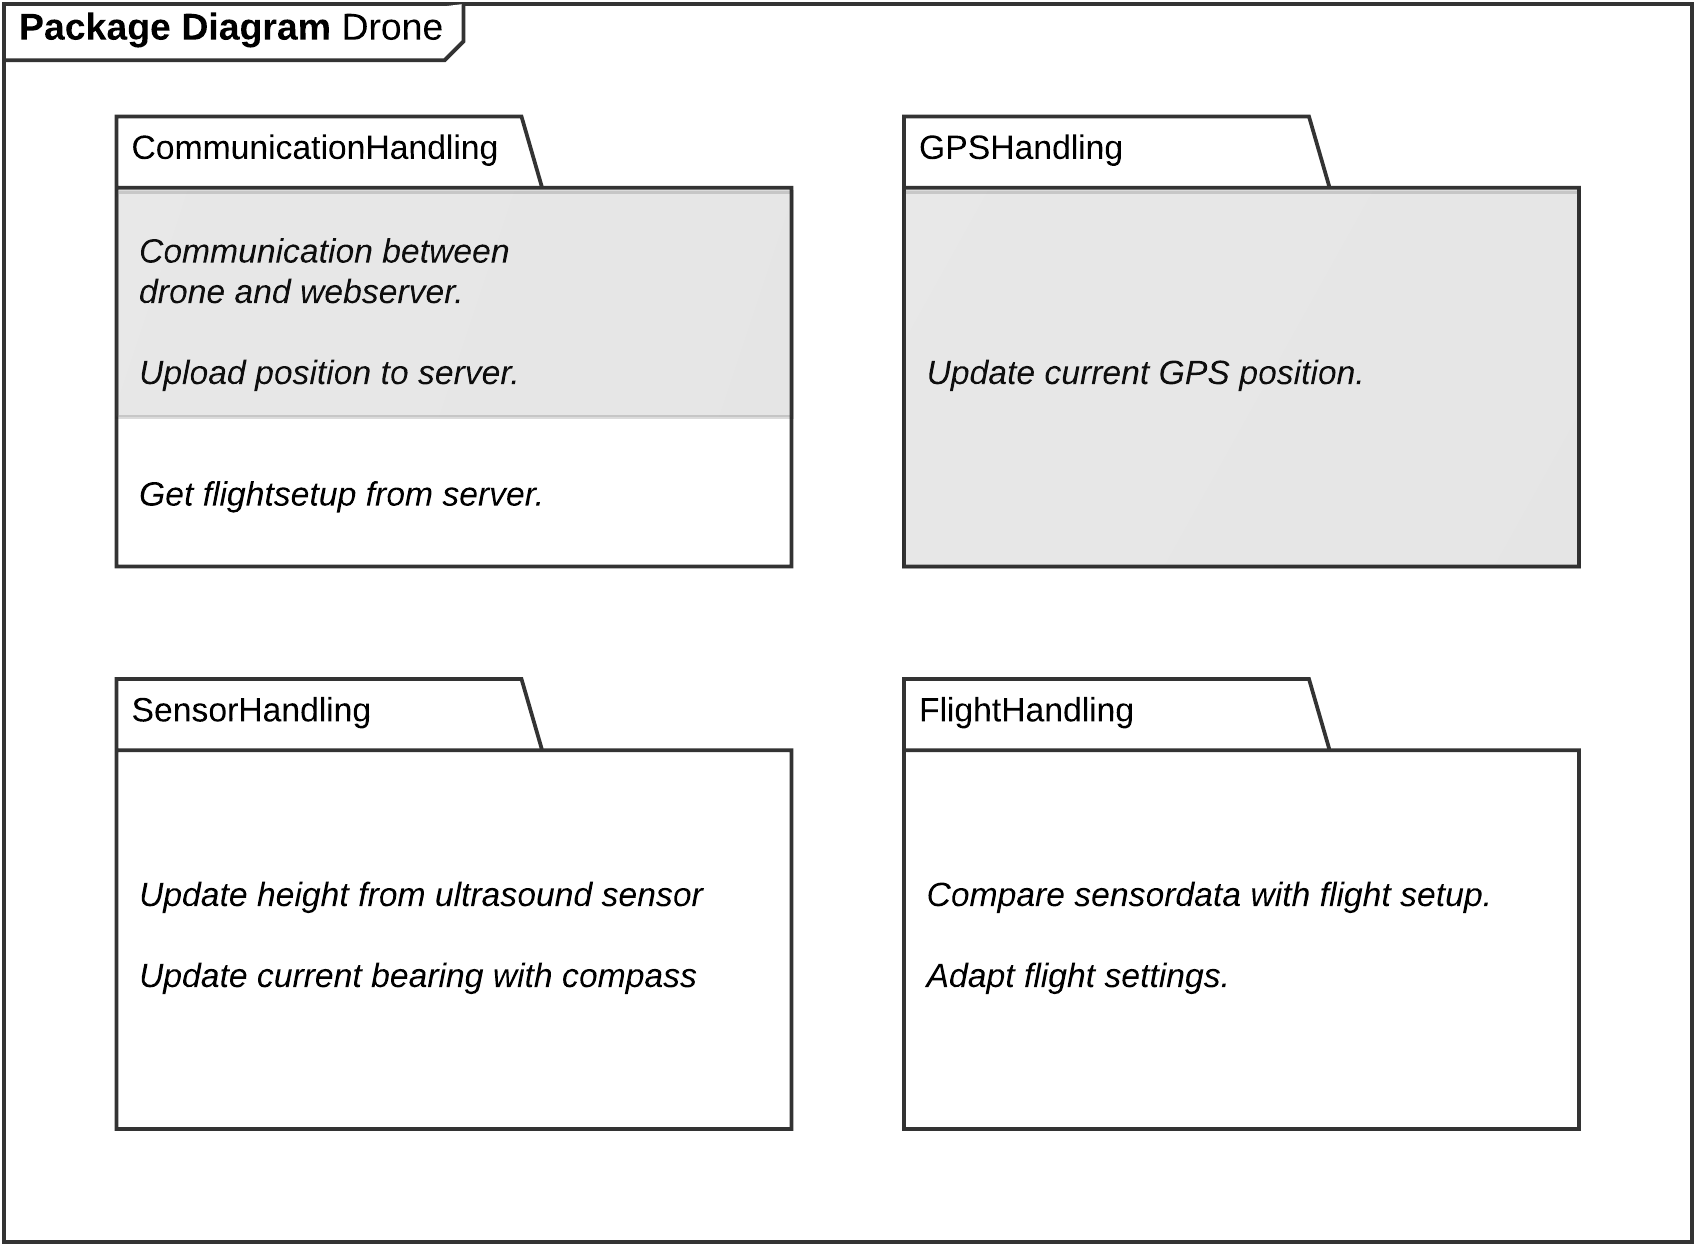
\includegraphics[width=1\textwidth]{Billeder/pakke_diagrammer/iteration2_drone.png}
	\vspace{-0.5cm}
	\caption{Pakkediagram drone}
	\label{fig:iteration2_pakke_diagram_drone}
\end{figure}

\textbf{CommunicationHandling}\\
Pakkens ansvar er kommunikation imellem drone og server. Efter denne iteration skal dronen både kunne hente flyveopsætninger fra server og sende sin nuværende GPS position til server.

\textbf{GPSHandling}\\
Pakkens ansvar er håndtering af GPS. Dels er pakken ansvarlig for opstart og initiering af GPS, og desuden bruges pakken hver gang dronens nuværende GPS position skal opdateres.

\textbf{SensorHandling}\\
Pakken er ansvarlig for indsamling af sensor data. I denne iteration skal pakken bruges til aflæsning af højdemåler og kompasset på flight control boardet. 

\textbf{FlightHandling}\\
Pakkens ansvar er kontrol og styring af drone under flyvning. Ved sammenligning af sensor data og data fra flyveopsætning tilpasses flyvehøjde, orientering mm



\newpage
\subsubsection*{Pakkediagram webapplikation}

I dette afsnit vises pakkediagram tilhørende webapplikation. De pakker der vises i pakkediagrammet består af en eller flere klasser, der med stort samspil udfører opgaver indenfor et fælles ansvarsområde. På hver pakke findes en lille beskrivelse, der tydeliggør pakkens ansvarsområde. De dele af pakkerne der er gråskraveret, er funktionalitet udarbejdet i tidligere iteration.

\begin{figure}[H]
	\centering
	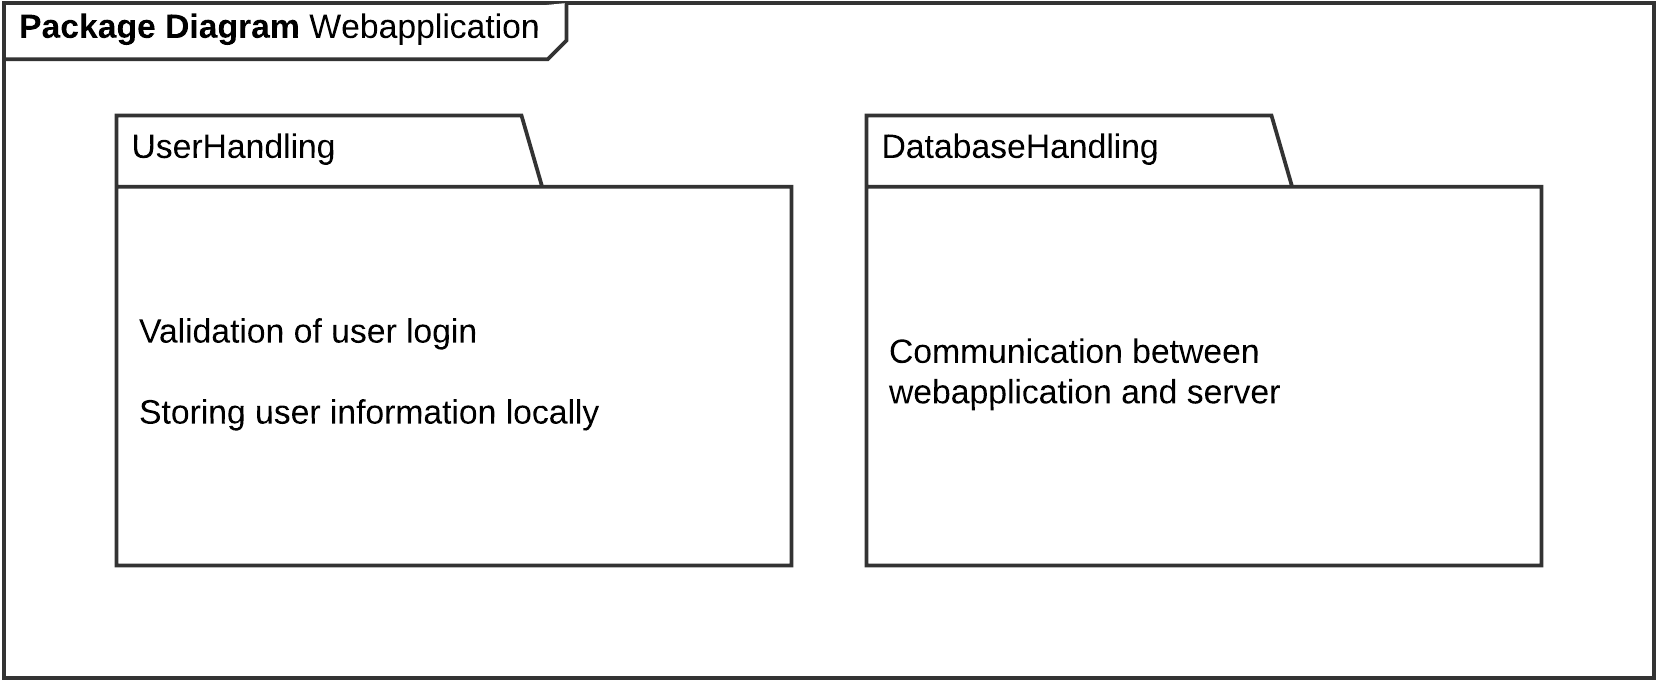
\includegraphics[width=1\textwidth]{Billeder/pakke_diagrammer/iteration1_server.png}
	\vspace{-0.5cm}
	\caption{Overordnet pakke diagram over webapplikationen}
	\label{fig:iteration1_pakke_diagram_webapp}
\end{figure}

\textbf{UserHandling}\\
Pakkens ansvar er validering af login/log ud på websitet. Pakken har også ansvaret for at hente og gemme data om den pågældende bruger.

\textbf{DatabaseHandling}\\
Pakkens ansvar er kommunikation imellem databasen og serveren. 

\textbf{DroneHandling}\\
Pakkens ansvar er alt data vedrørende dronen, så som håndteringen af events, waypoints og div droner.

\newpage

\subsubsection*{Sekvensdiagram drone}

Til iteration 2 er systemsekvensen beskrevet med 3 mindre sekvensdiagrammer i stedet for 1 stort. Ydermere er der lavet 2 sekvens diagrammer der går mere i dybden med 3G modulet og dens klasser. 
Denne fremstilling gør det muligt at repræsentere systemets funktionalitet på mere overskuelig vis, hvilket indirekte øger forståelsen af diagrammerne. Hvert af de 3 overordnede sekvensdiagrammer bruges til at fortælle hvordan en delmængde af systemet fungerer.

Af figur \ref{fig:Sekvens_diagram_iteration2_1} fremgår det hvordan bruger opretter en ny flyveopsætning. Det vises desuden hvilke interaktioner der foretages mellem bruger og website, samt hvordan server løbende indgår og benyttes i sekvensen. 

%kommentar
\begin{figure}[H]
	\centering
	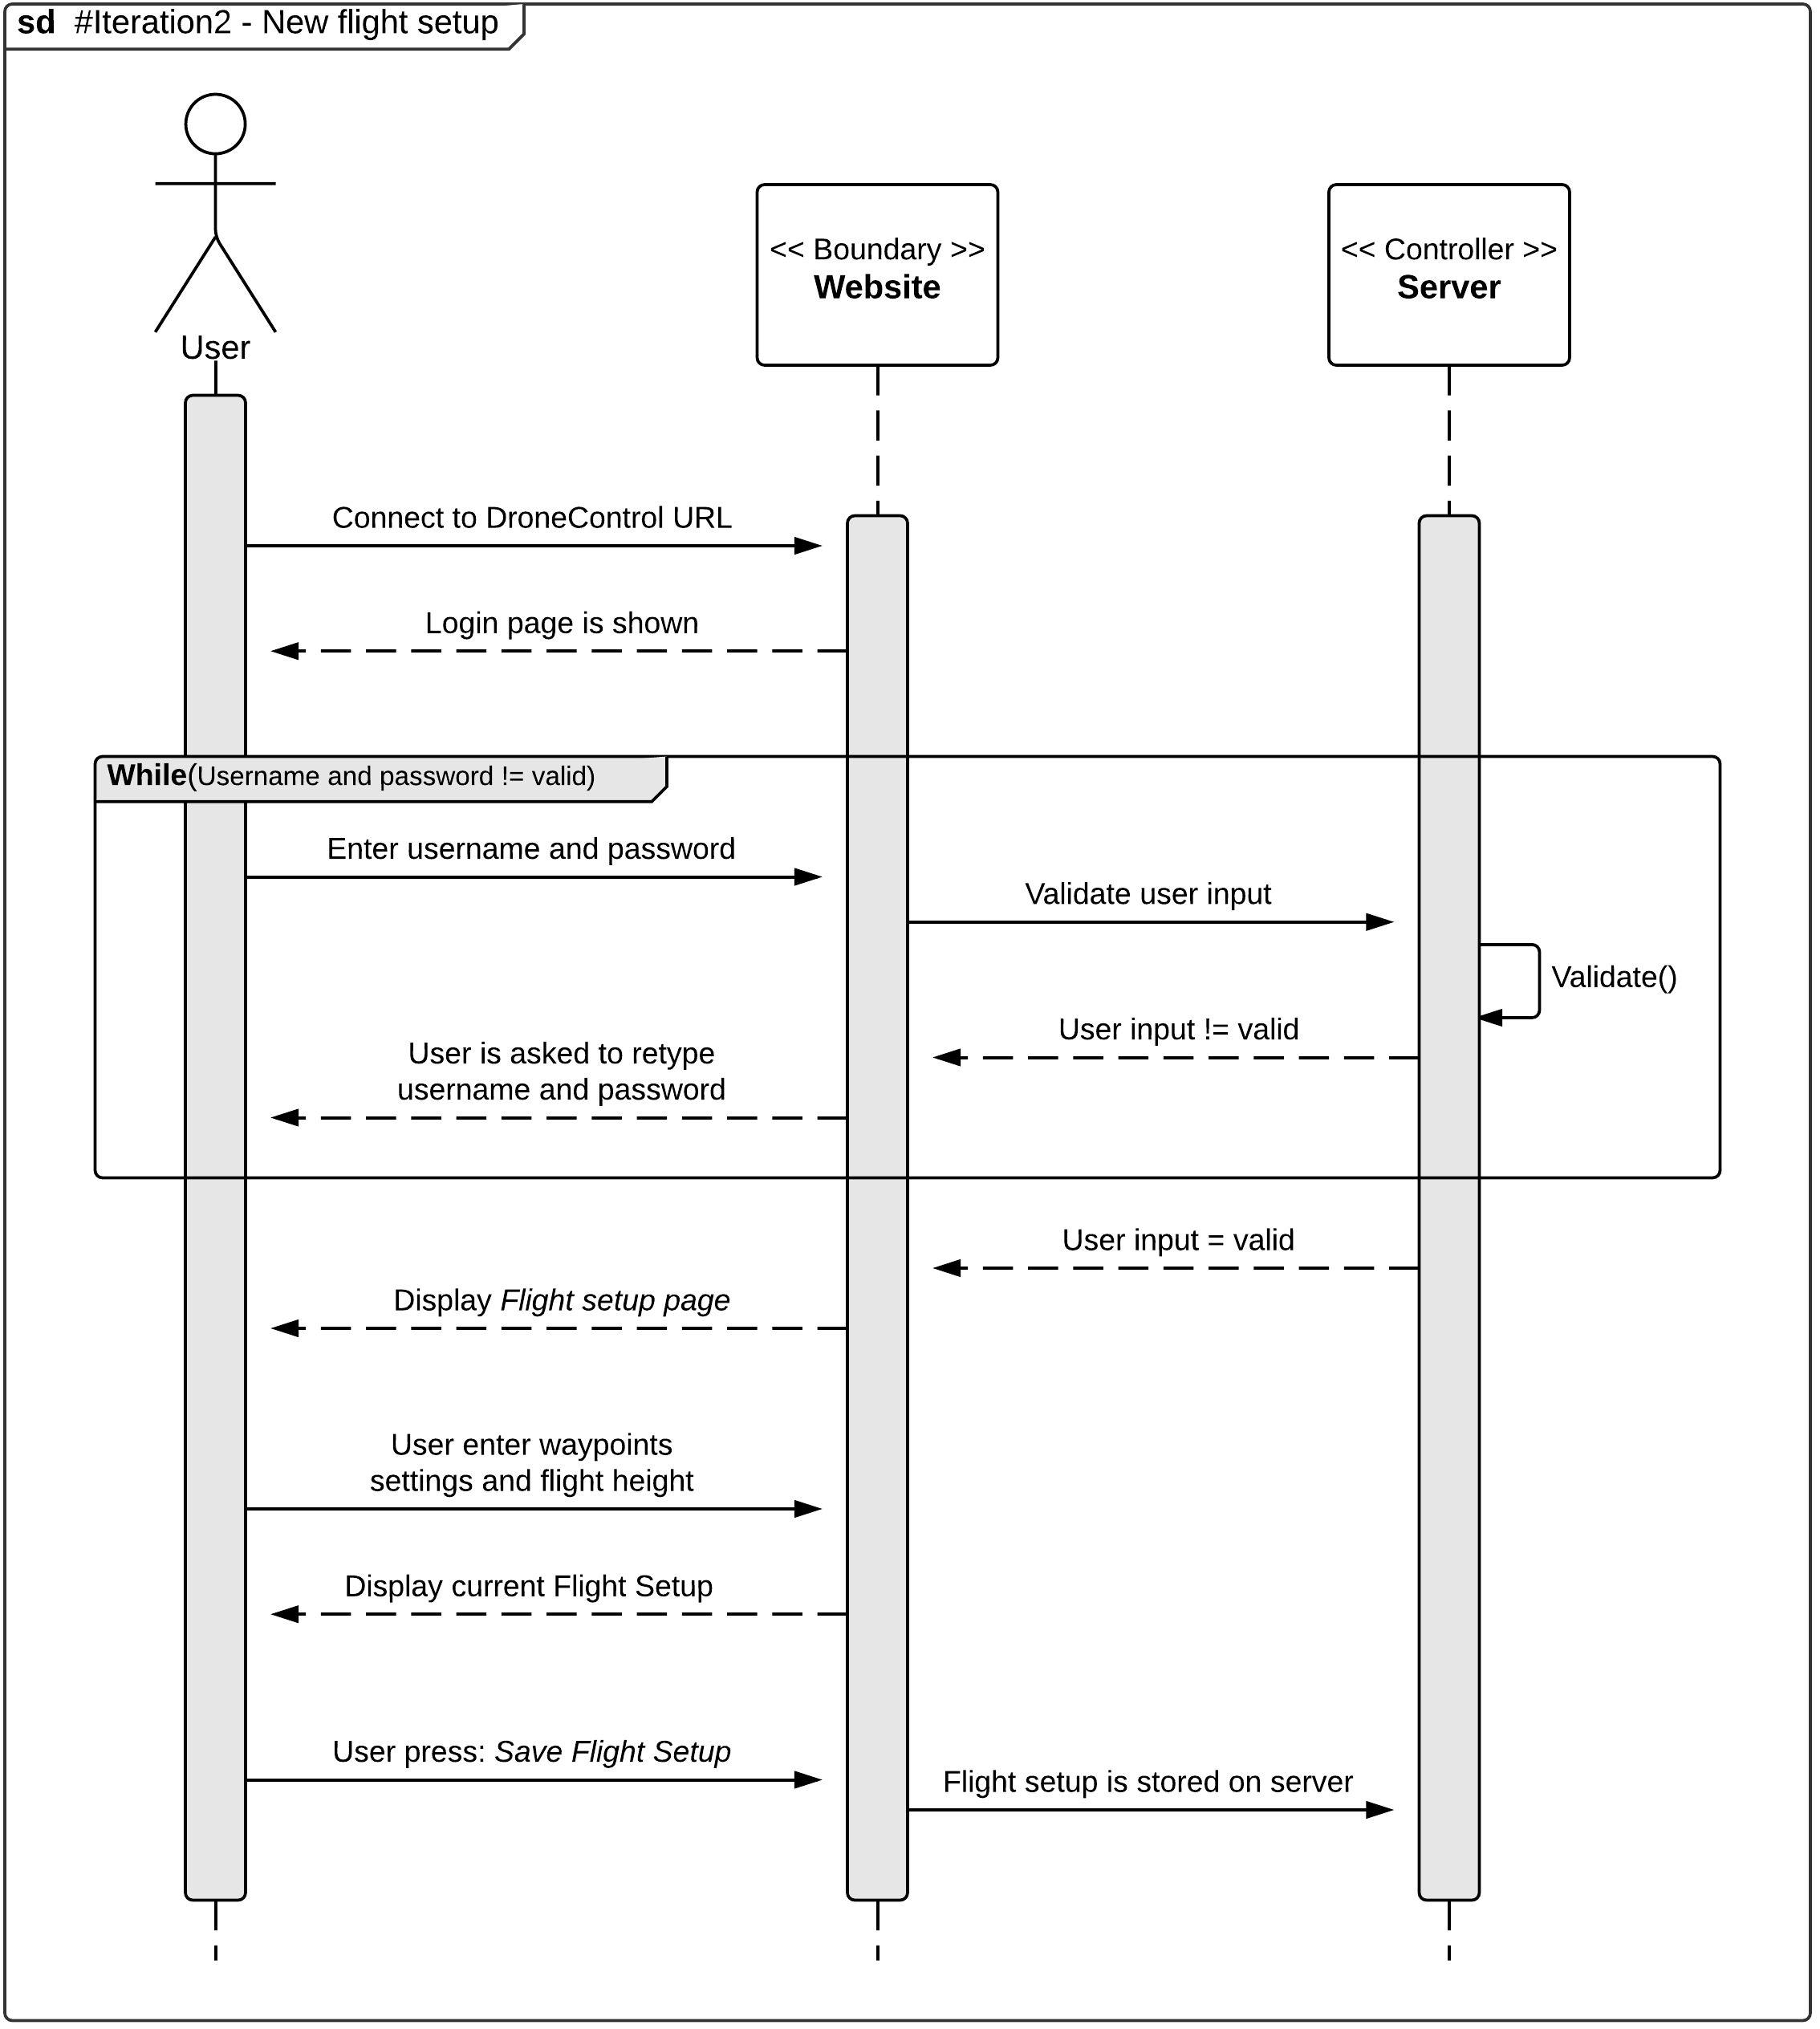
\includegraphics[width=1\textwidth]{Billeder/sekvens/sekvens_iteration2_1}
	\caption{Sekvensdiagram \#iteration 2}
	\label{fig:Sekvens_diagram_iteration2_1}
\end{figure}


\newpage

På figur \ref{fig:Sekvens_diagram_iteration2_2} fremgår det hvordan dronens main controller via 3G-shieldet kommunikerer med serveren for at kontrollere om der er en ny flyveopsætning tilgængelig. Det vises også hvilke beskeder der flyder frem og tilbage mellem main controller og server. Desuden vises det at dronen først henter ny flyveomsætning, når serveren har bekræftet, at der er en flyveopsætning tilgængelig.   

%kommentar
\begin{figure}[H]
	\centering
	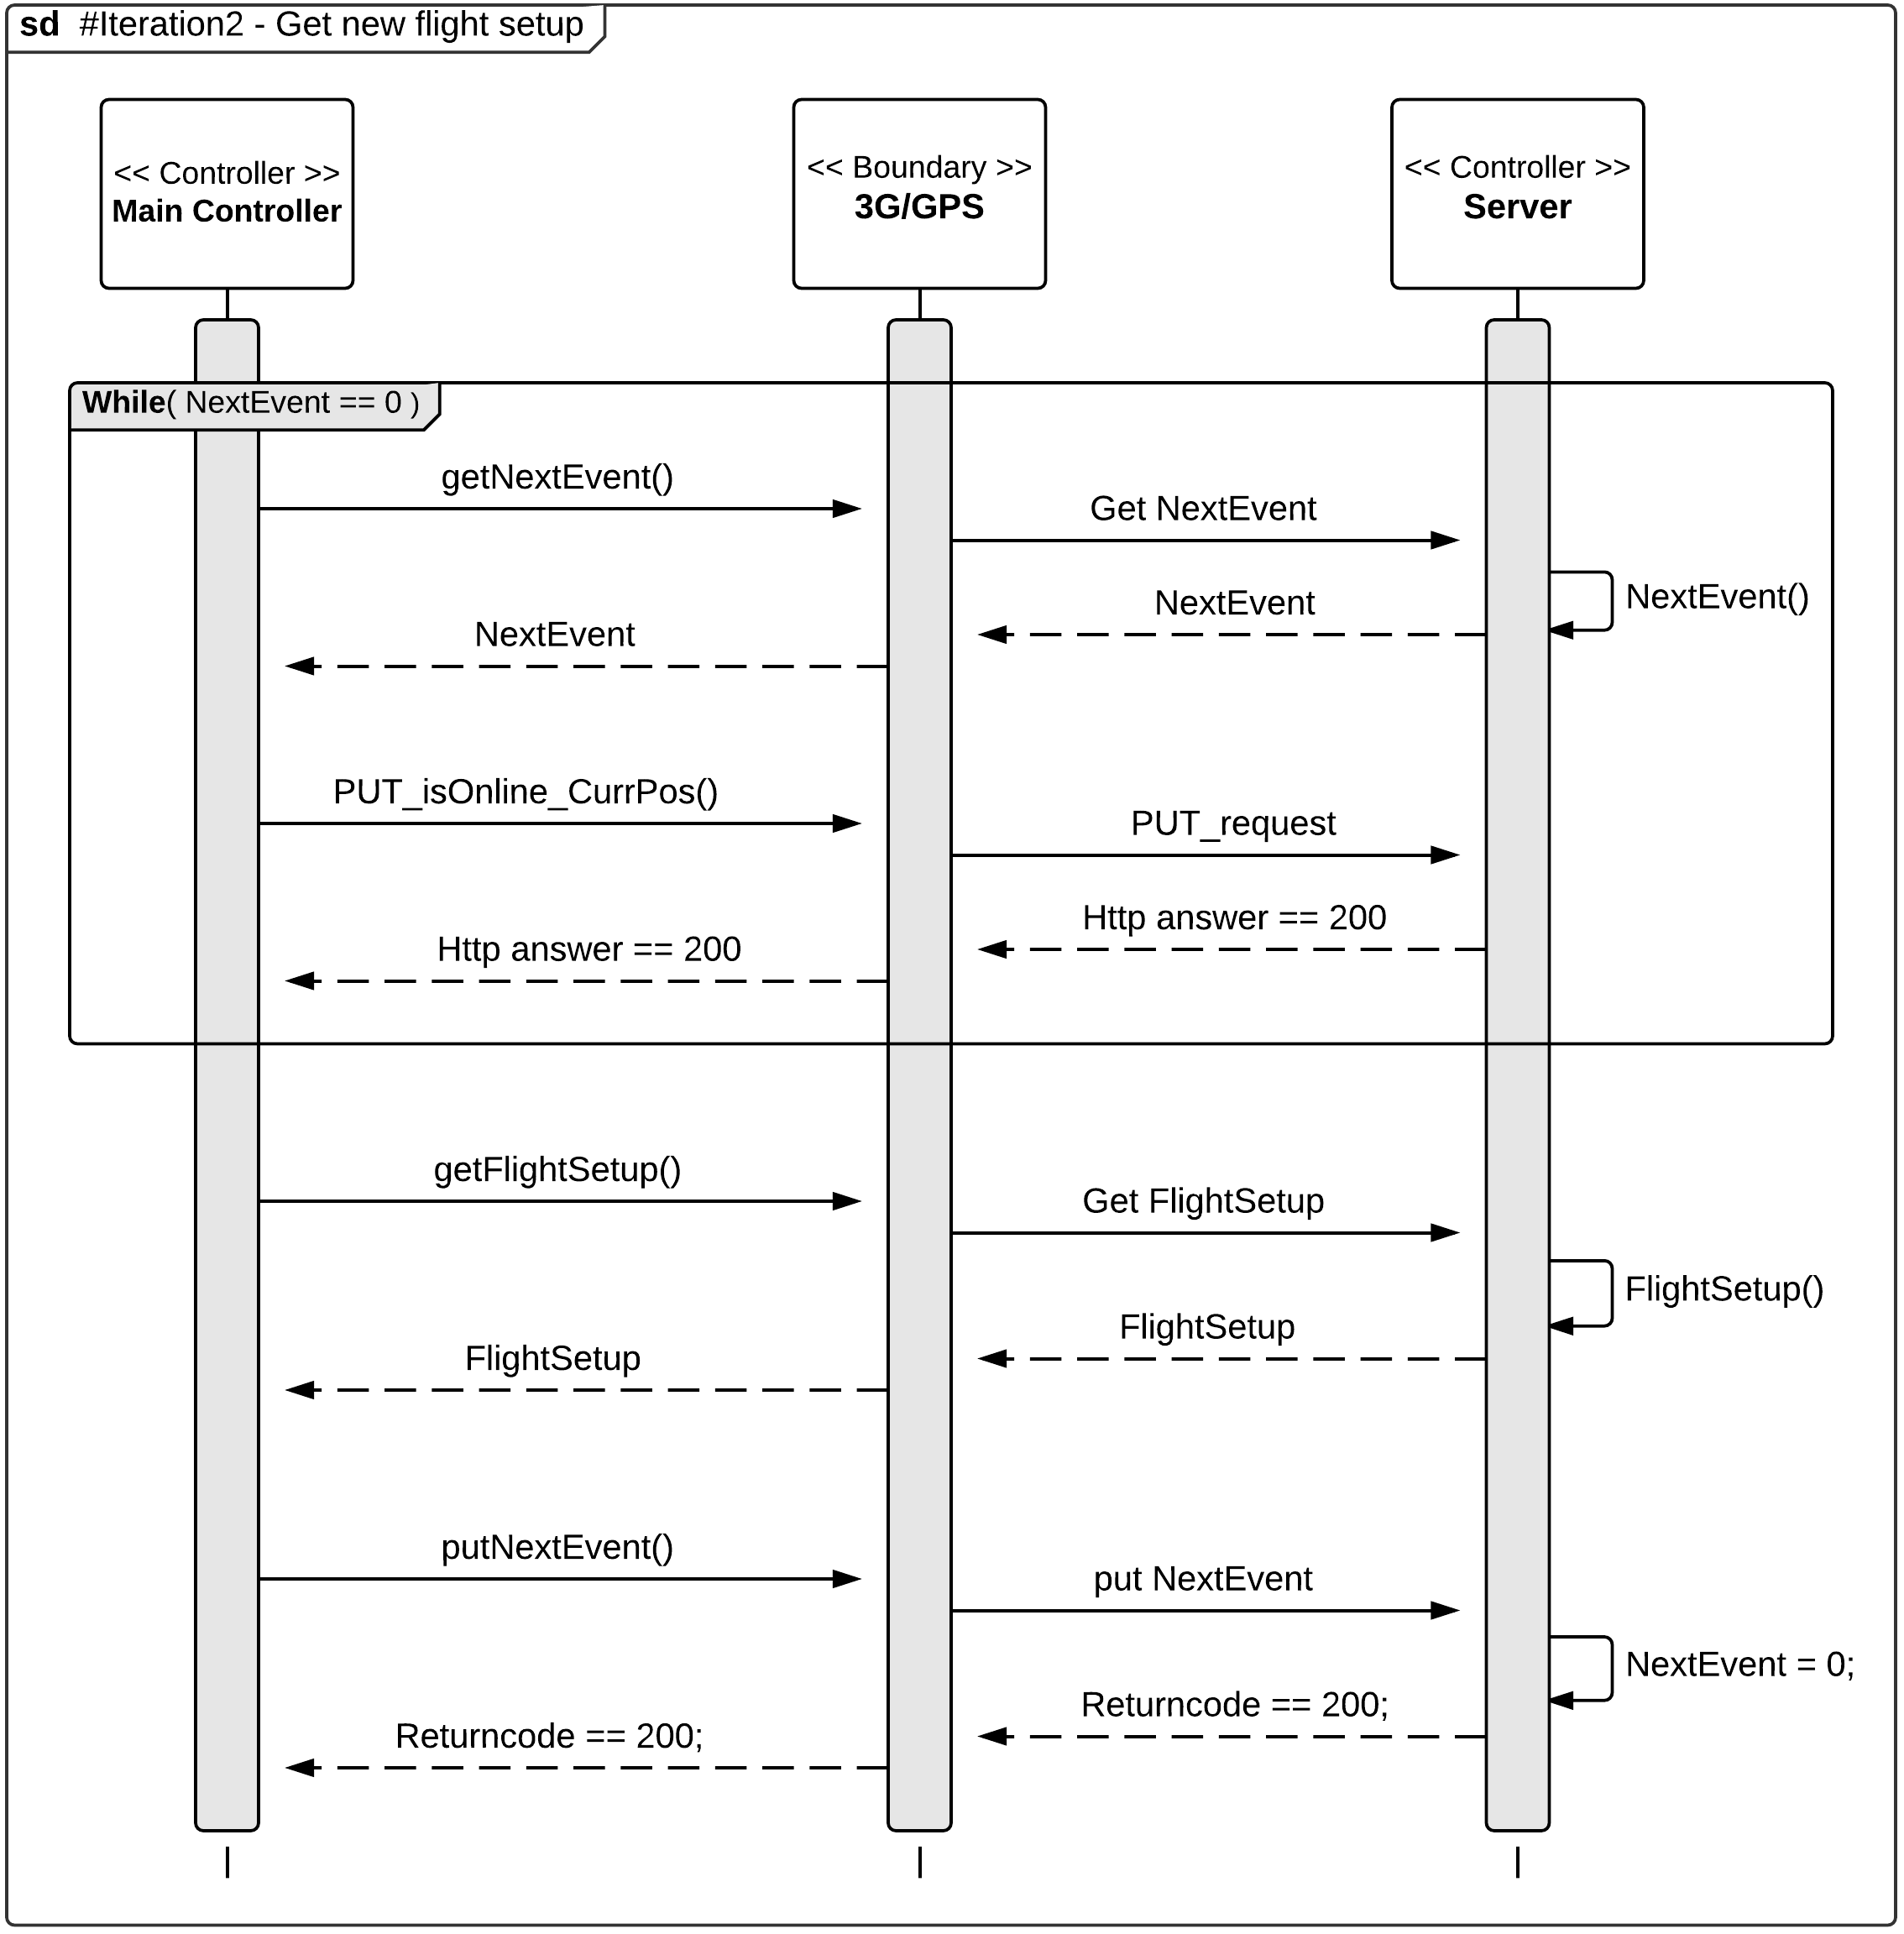
\includegraphics[width=1\textwidth]{Billeder/sekvens/sekvens_iteration2_2}
	\caption{Sekvensdiagram \#iteration 2}
	\label{fig:Sekvens_diagram_iteration2_2}
\end{figure}

\newpage

På Figur \ref{fig:Sekvens_getwaypoints} ses en mere detaljeret beskrivelse af 3G modulets klasser. Disse klasser håndterer al kommunikation mellem drone og server.

\begin{figure}[H]
	\centering
	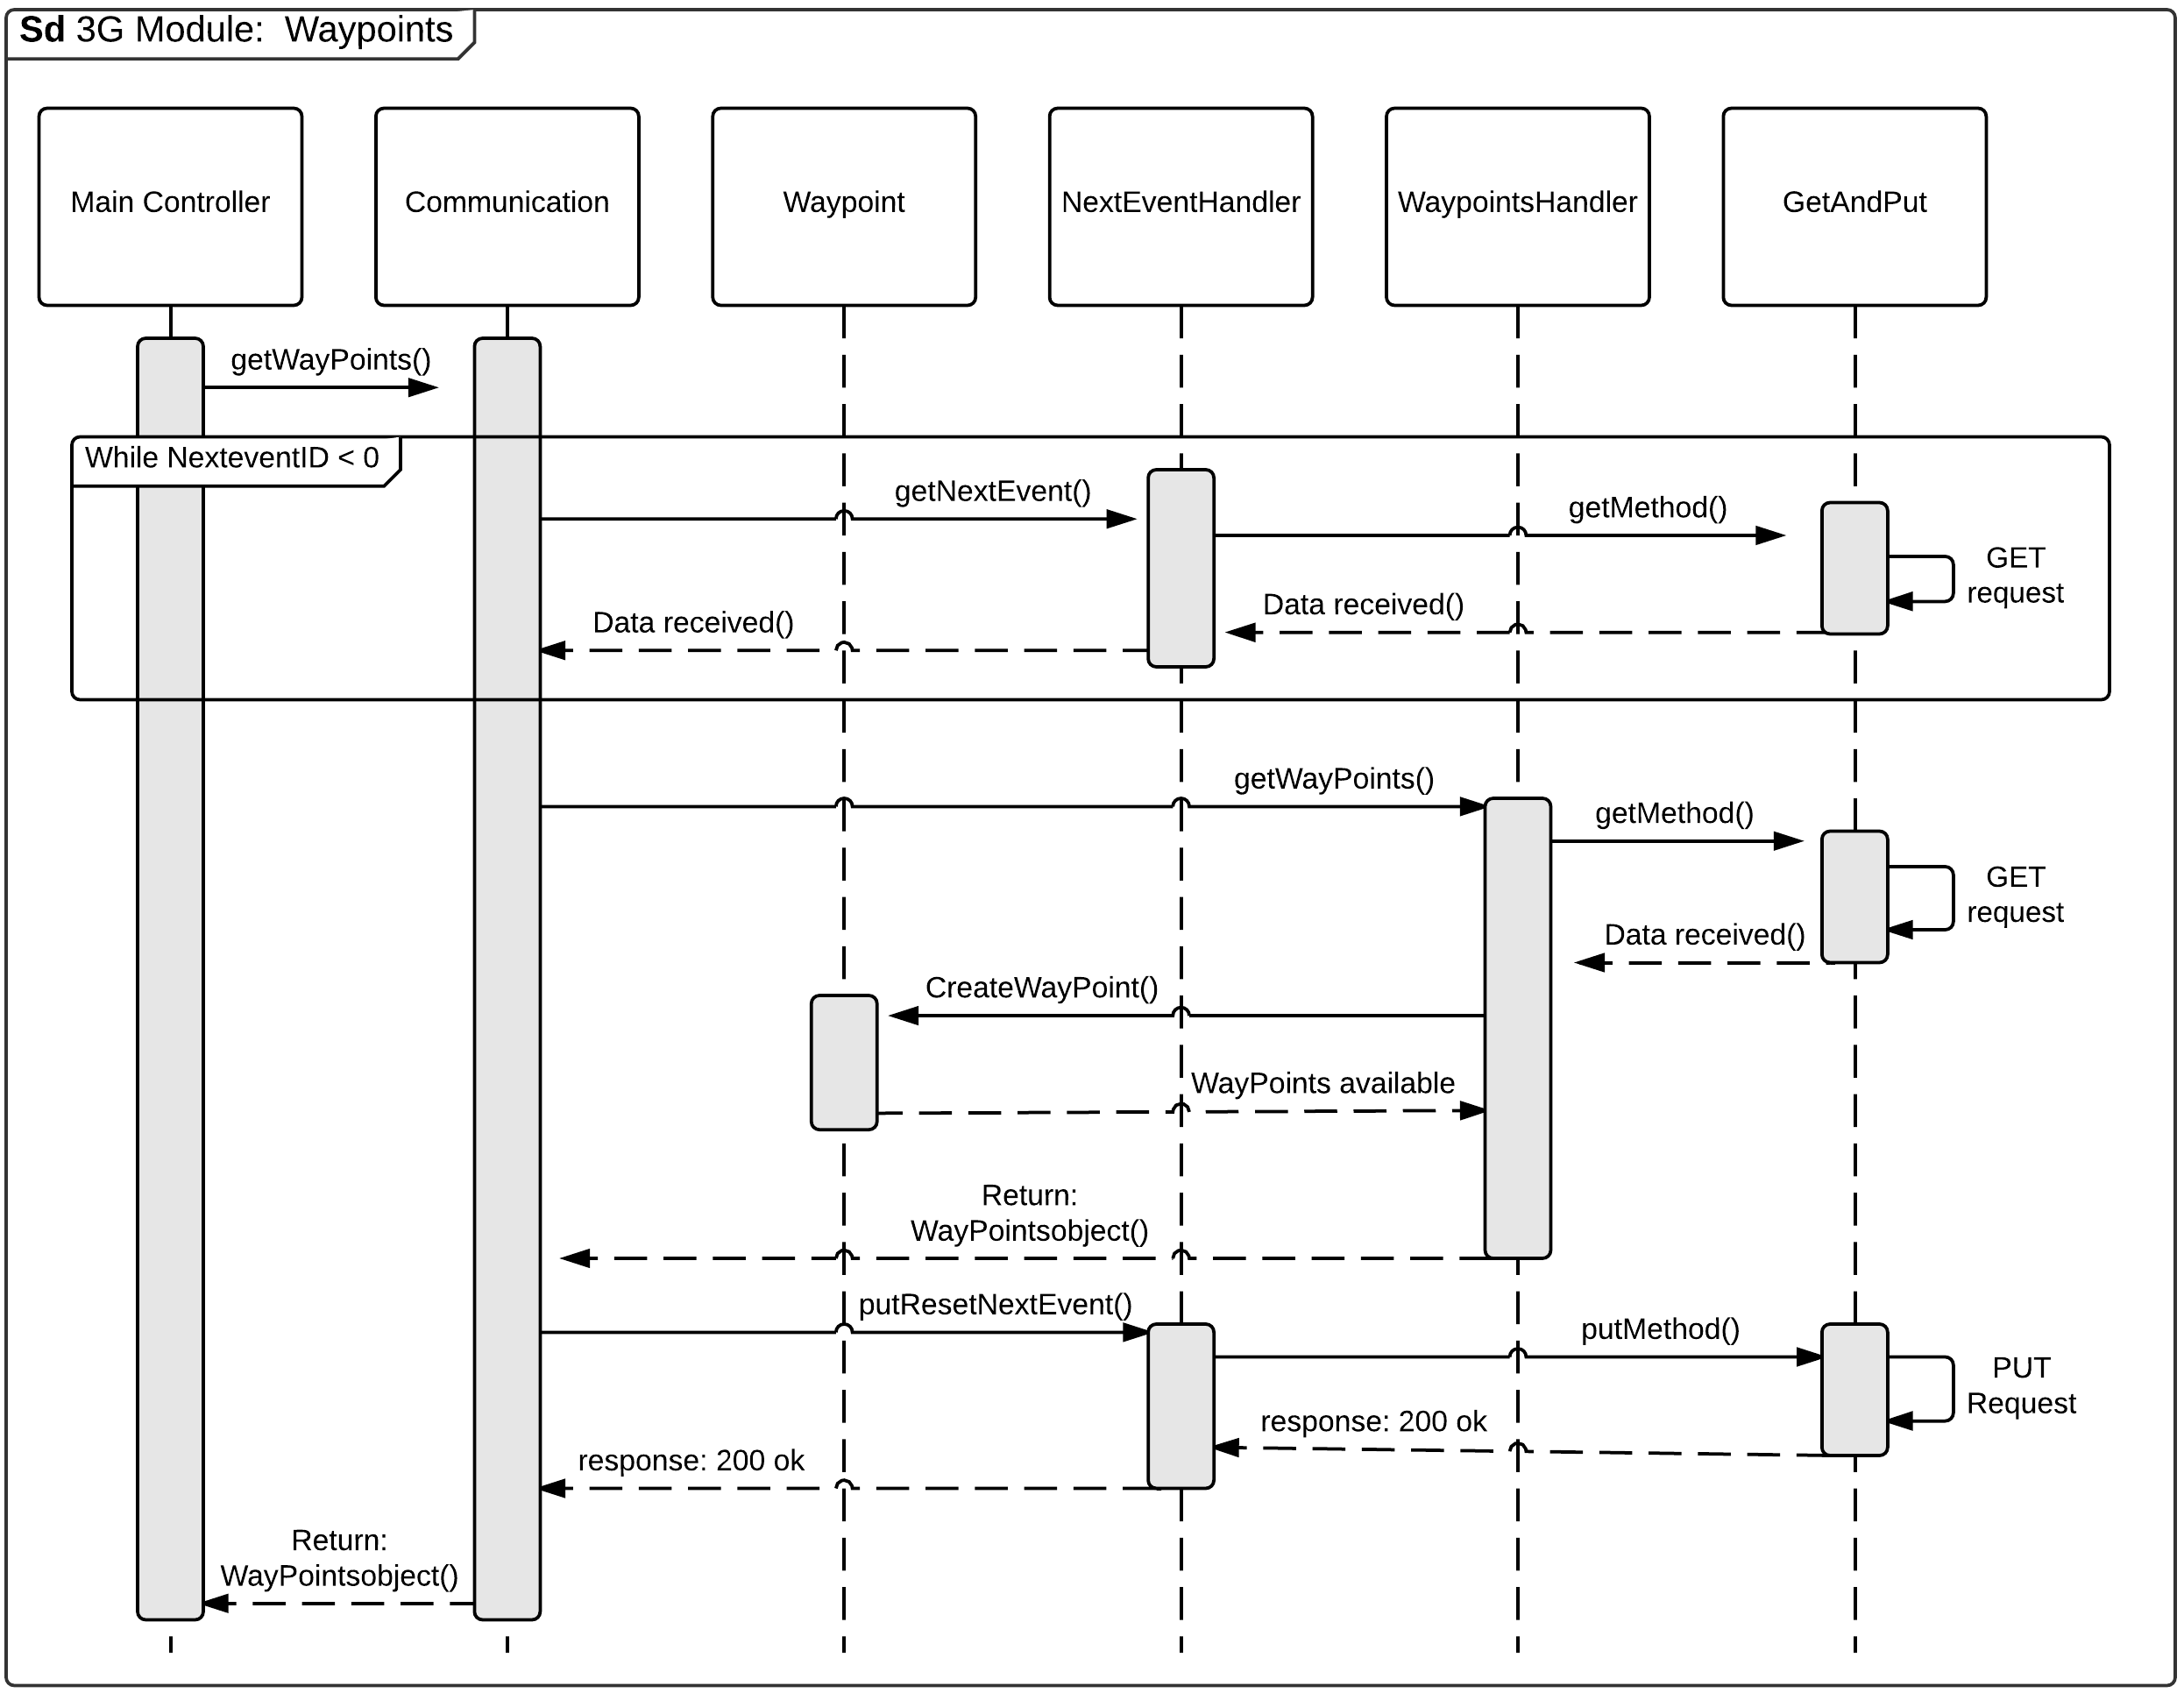
\includegraphics[width=1\textwidth]{Billeder/sekvens/sekvens_getwaypoints.png}
	\caption{Sekvensdiagram udvidet 3G module - getwaypoints}
	\label{fig:Sekvens_getwaypoints}
\end{figure}

\newpage

Af figur \ref{fig:Sekvens_diagram_iteration2_3} fremgår det hvordan dronen opererer når den flyver autonomt mod en givet GPS position. Main controlleren indsamler kompas data fra flight control boardet, latitude og longitude fra 3G/GPS modulet og flyvehøjde fra ultralyds sensoren. Den indhentede data processeres og bruges til at korrigerer de nuværende flyveindstillinger.
Som det fremgår af while loopet fortsætter flyvningen indtil dronen er 15 meter fra den GPS destination bruger valgte i flyveopsætningen. 


%kommentar
\begin{figure}[H]
	\centering
	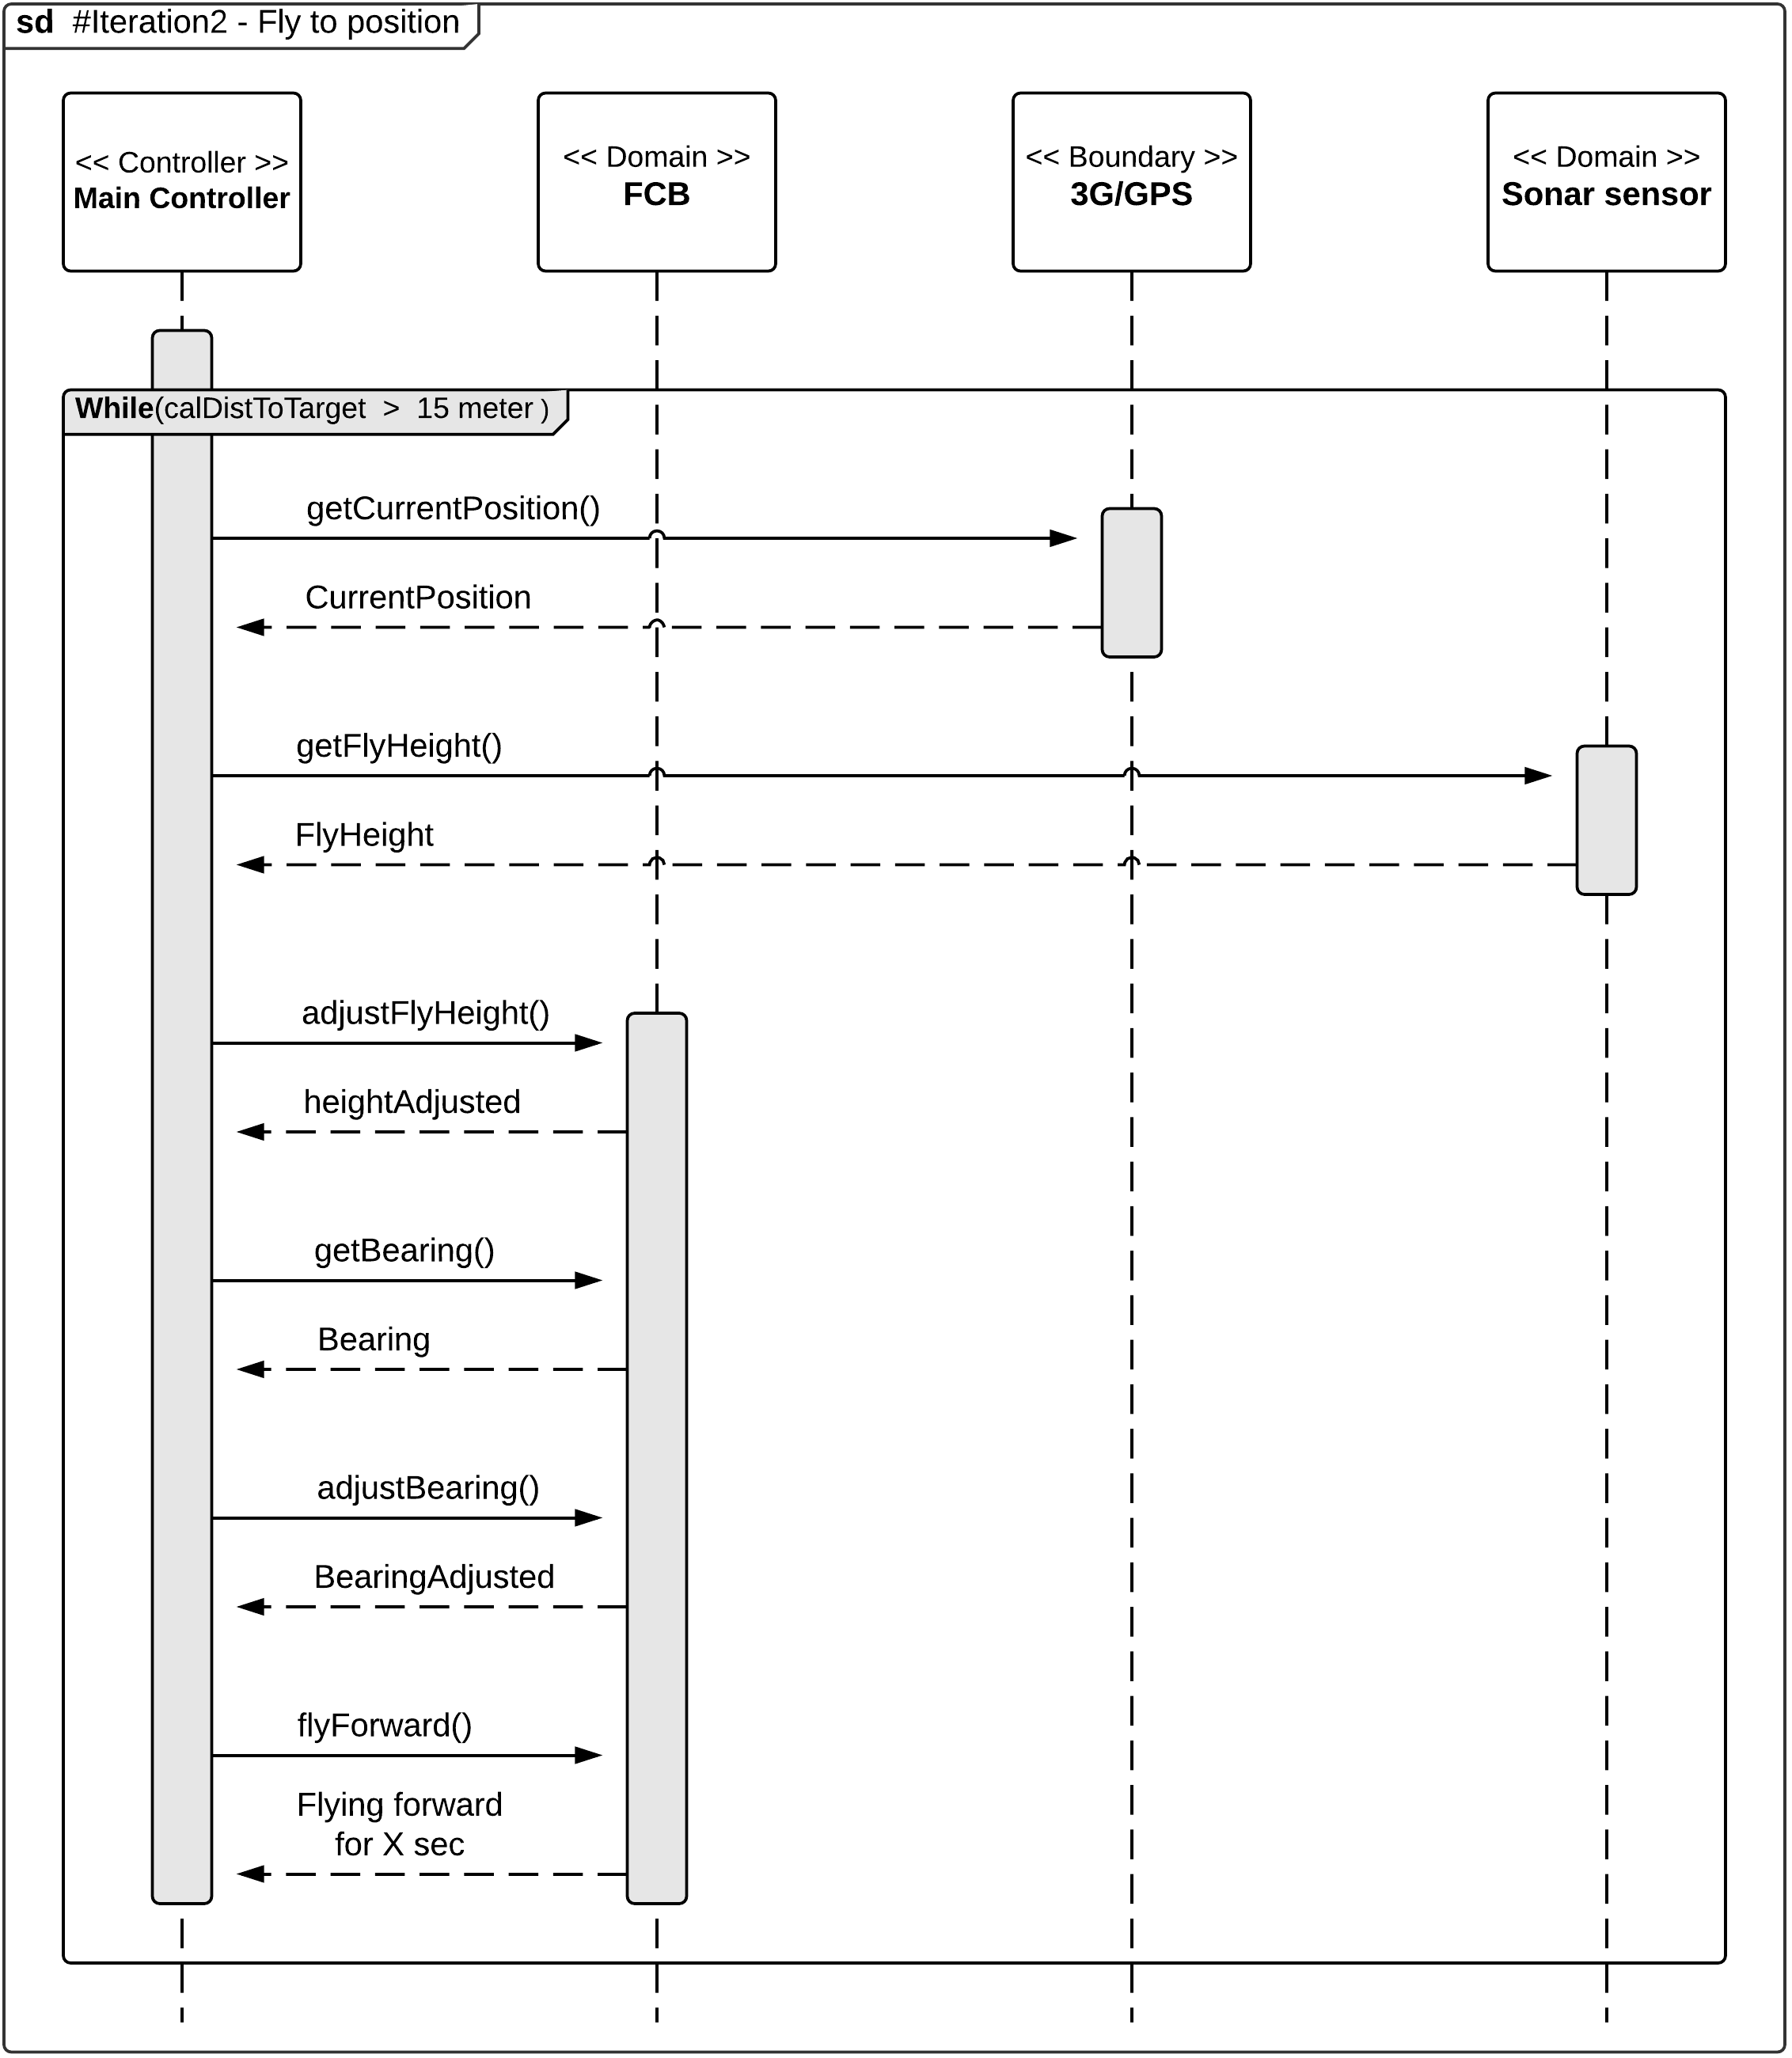
\includegraphics[width=1\textwidth]{Billeder/sekvens/sekvens_iteration2_3}
	\caption{Sekvensdiagram \#iteration 2}
	\label{fig:Sekvens_diagram_iteration2_3}
\end{figure}

\newpage
\subsubsection*{Sekvensdiagram webapplikation}
\vspace{-0.1cm}
På figur \ref{fig:page_load} ses hvordan klasserne på websitet interagere med hinanden ved et page load. Kortet bliver initialiseret med centrum over århus og drone markeren bliver initialiseret. Useren som blev gemt ved login bliver brugt til at give en velkomst besked oppe i højre hjørne og sener vil blive brugt når der skal oprettet nye events. Listen med tilgængelige droner bliver loaded. Et click event bliver også oprettet som trigger ved click på kortet til oprettelse af nye waypoints.
\begin{figure}[H]
	\centering
	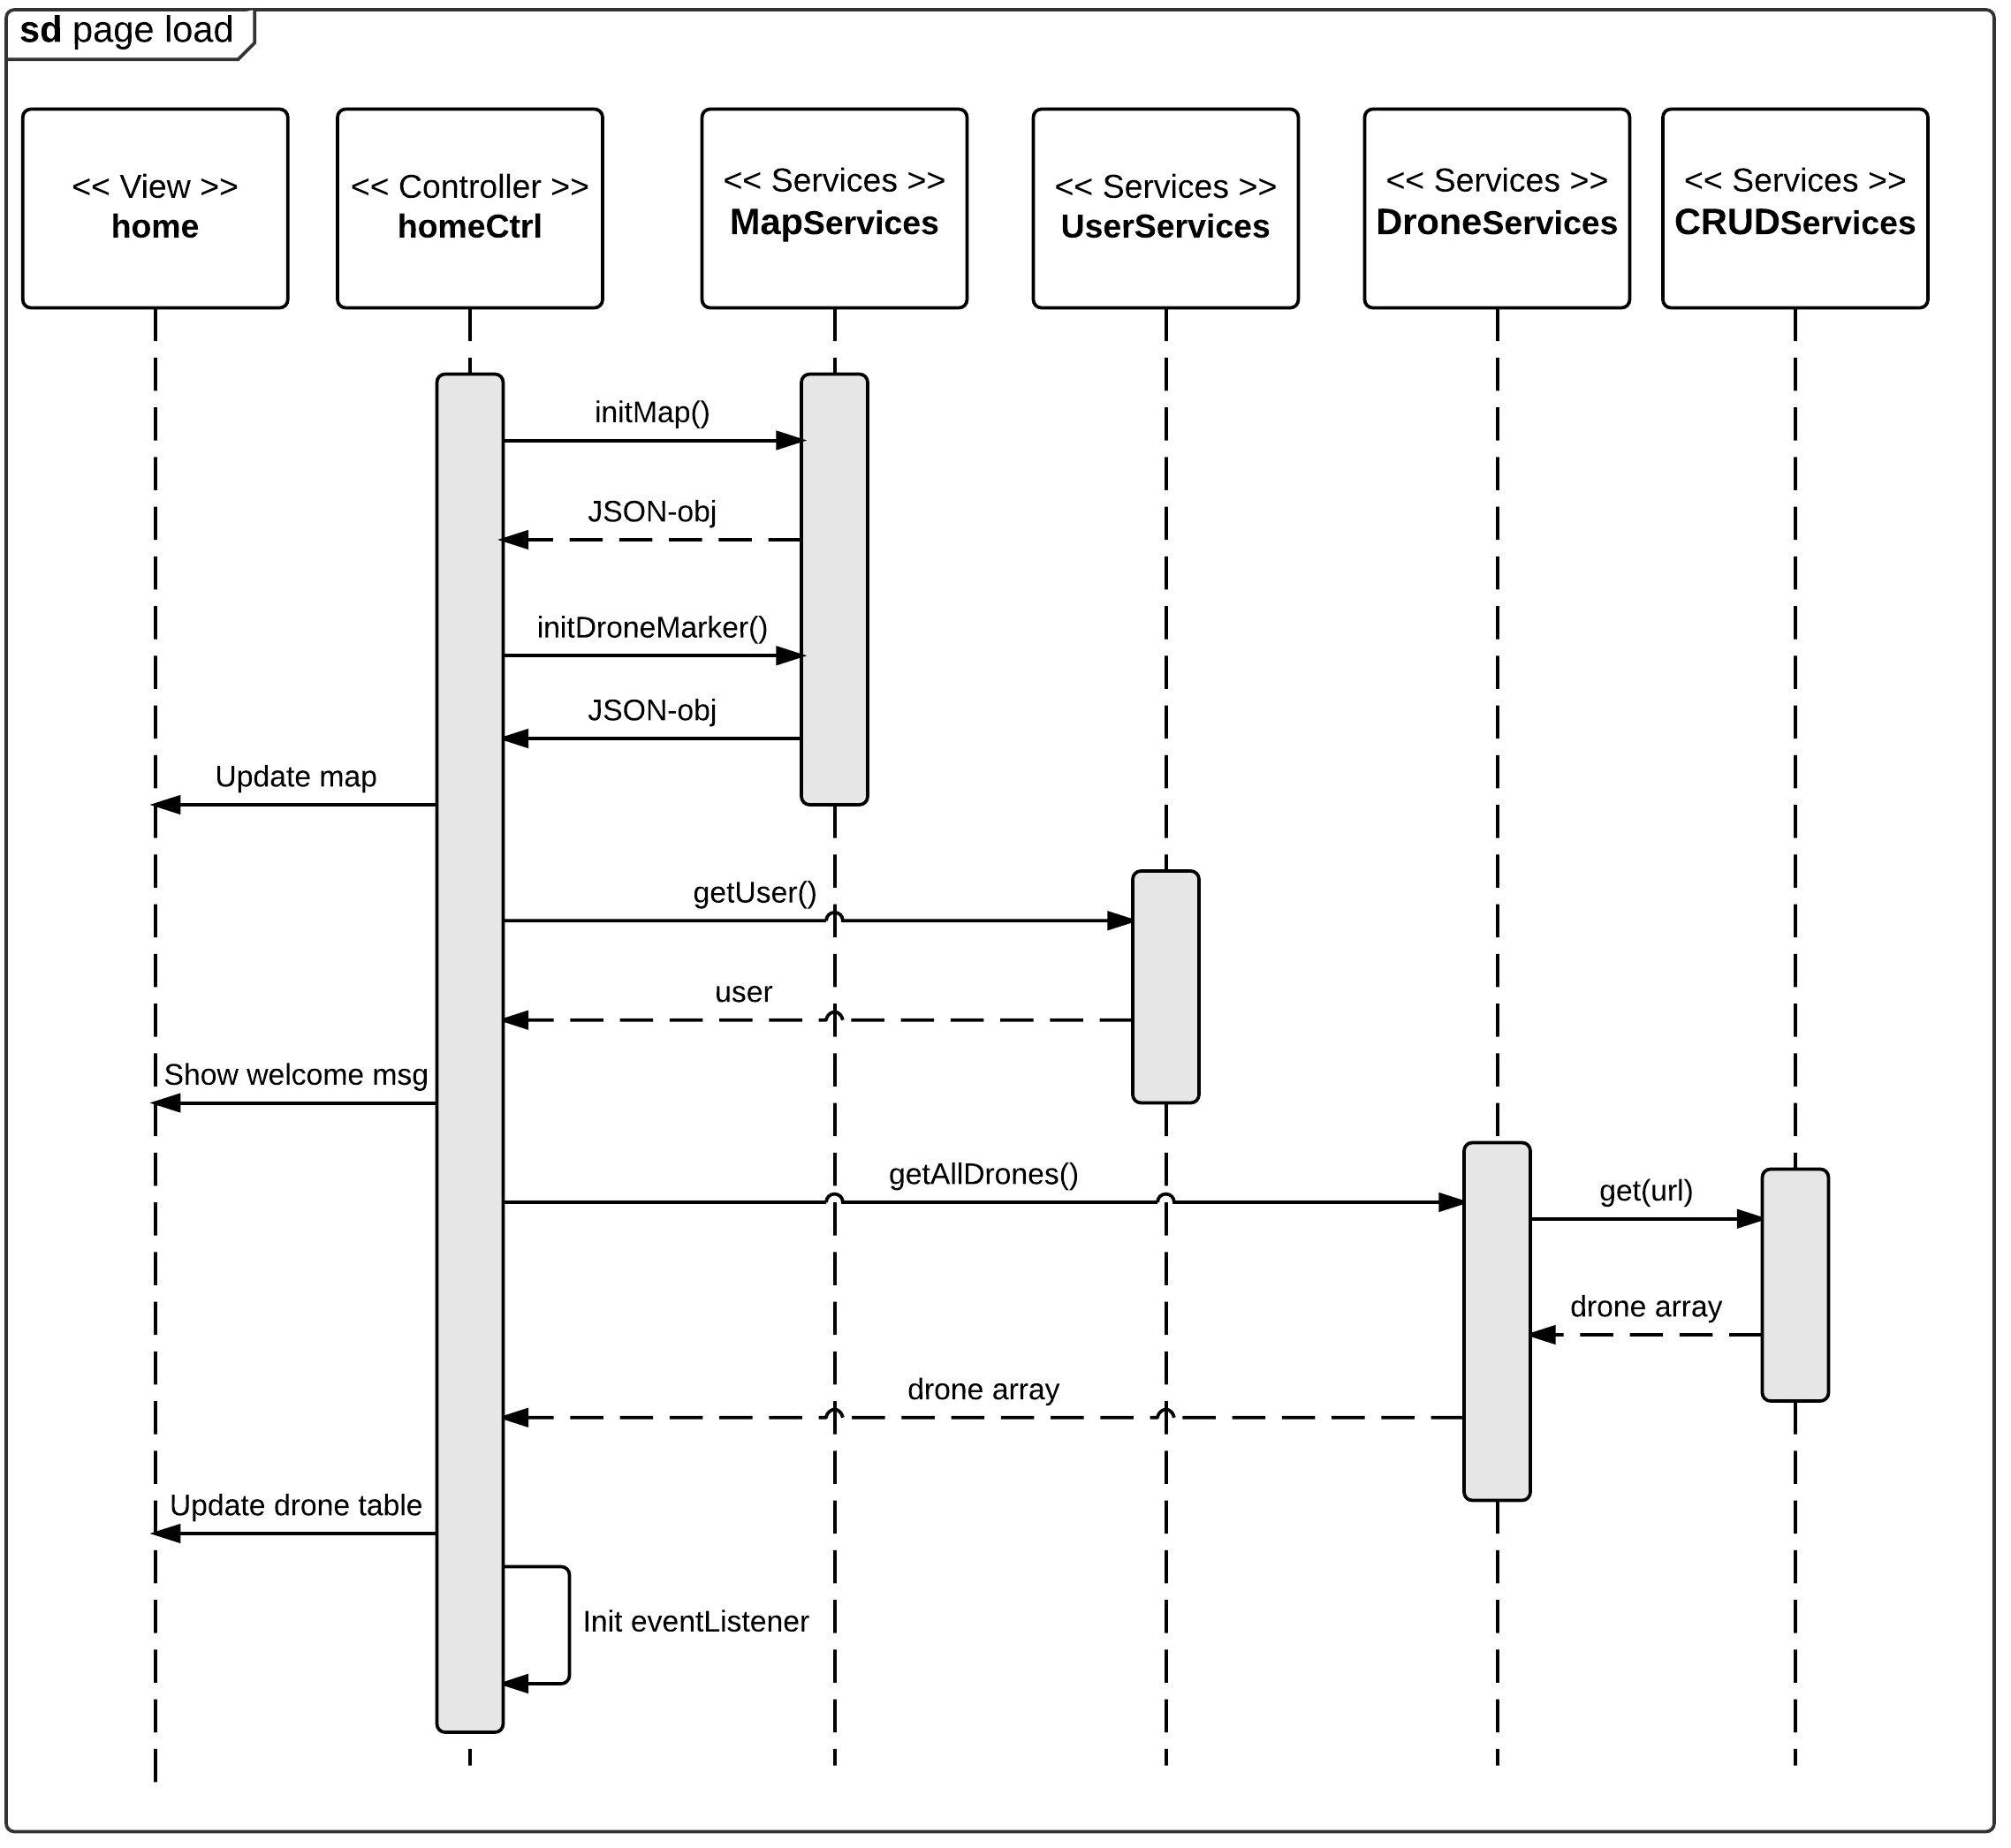
\includegraphics[width=1\textwidth]{Billeder/sekvens/sd_page_load.png}
	\caption{Sekvensdiagram page load}
	\label{fig:page_load}
\end{figure}

\newpage
På figur \ref{fig:send_waypoints} ses hvilke hændelser der finder sted i systemet, når useren trykker på "send event". Hvert services har et ansvar og det er dem der kommunikere ud til CRUD-servicesen, på den måde er logikken for data håndtering skubbet ud i div. services. 
\begin{figure}[H]
	\centering
	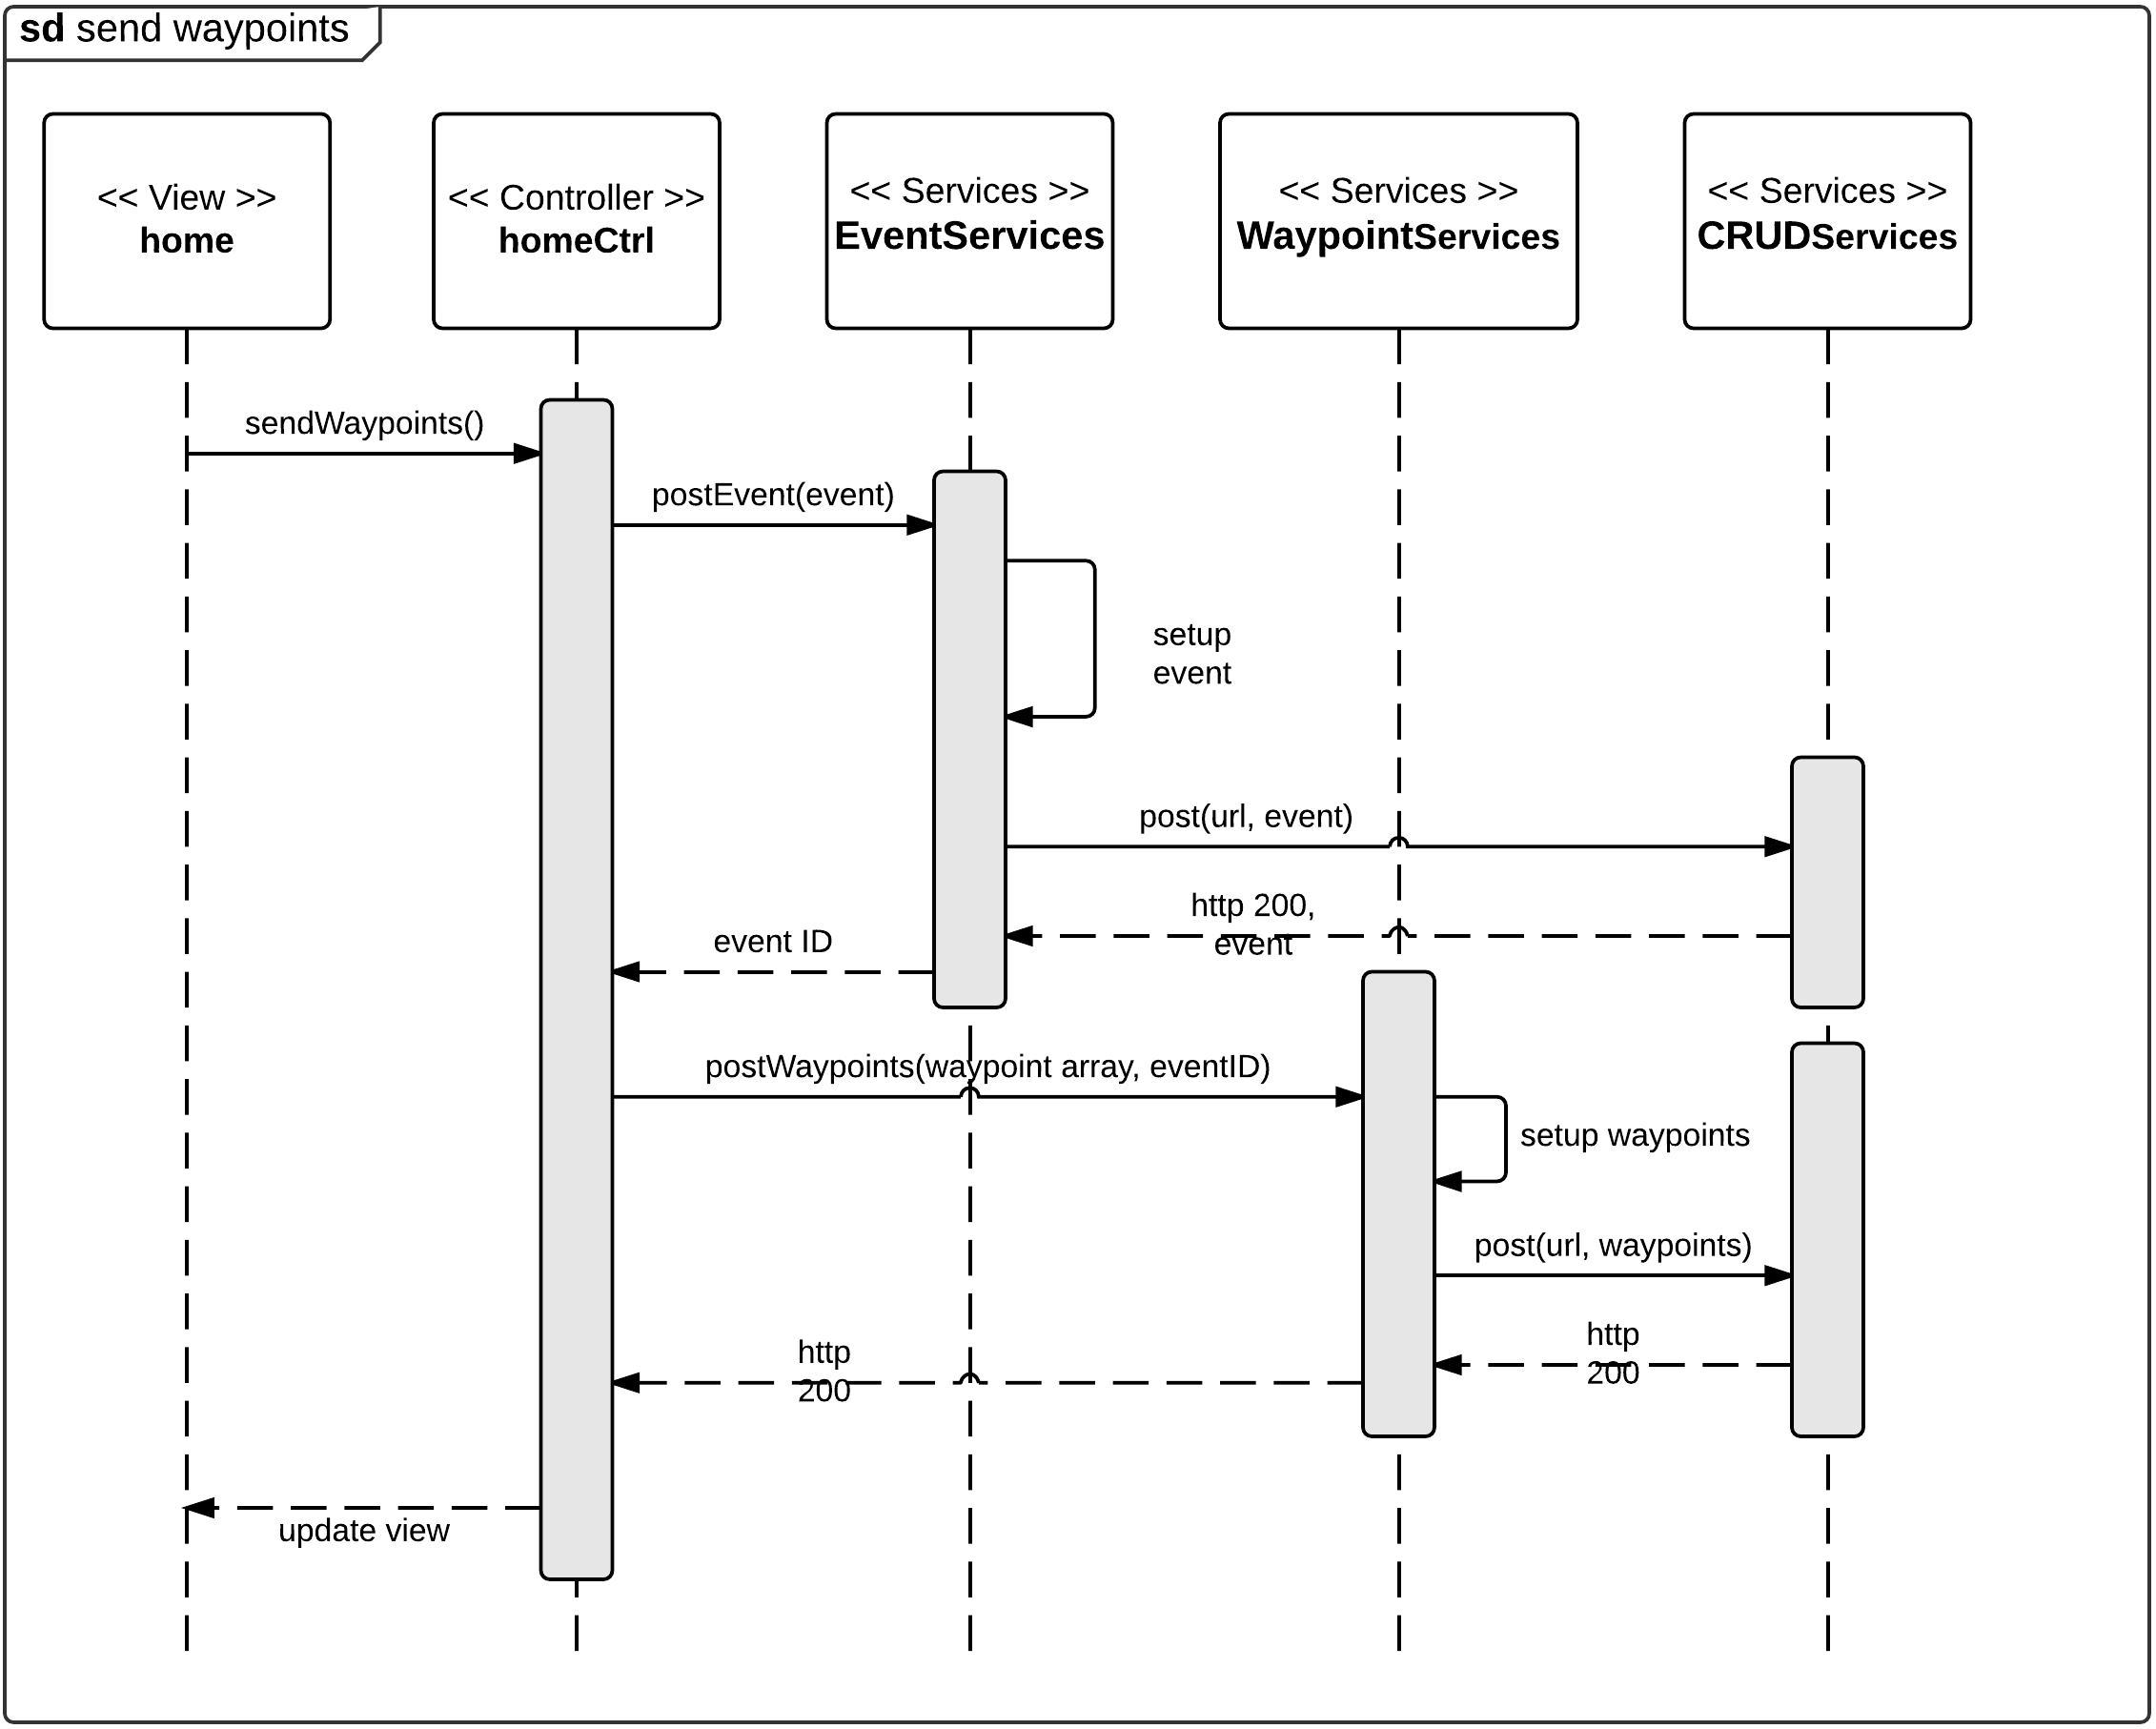
\includegraphics[width=1\textwidth]{Billeder/sekvens/sd_send_waypoints.png}
	\caption{Sekvensdiagram send waypoints}
	\label{fig:send_waypoints}
\end{figure}

\newpage
På figur \ref{fig:update_view} ses hvilke hændelser der finder sted i systemet, når useren trykker på forskellige droner i tabellen. Når et klik på tabellen finder sted skal view'et opdateret i forhold til den givet drone, dvs. hvis dronen har et event, så skal det vises og dertilhørende waypoints. Hvis der ikke er noget event tilknyttet til dronen skal useren have mulighed for at oprette et nyt event.
\begin{figure}[H]
	\centering
	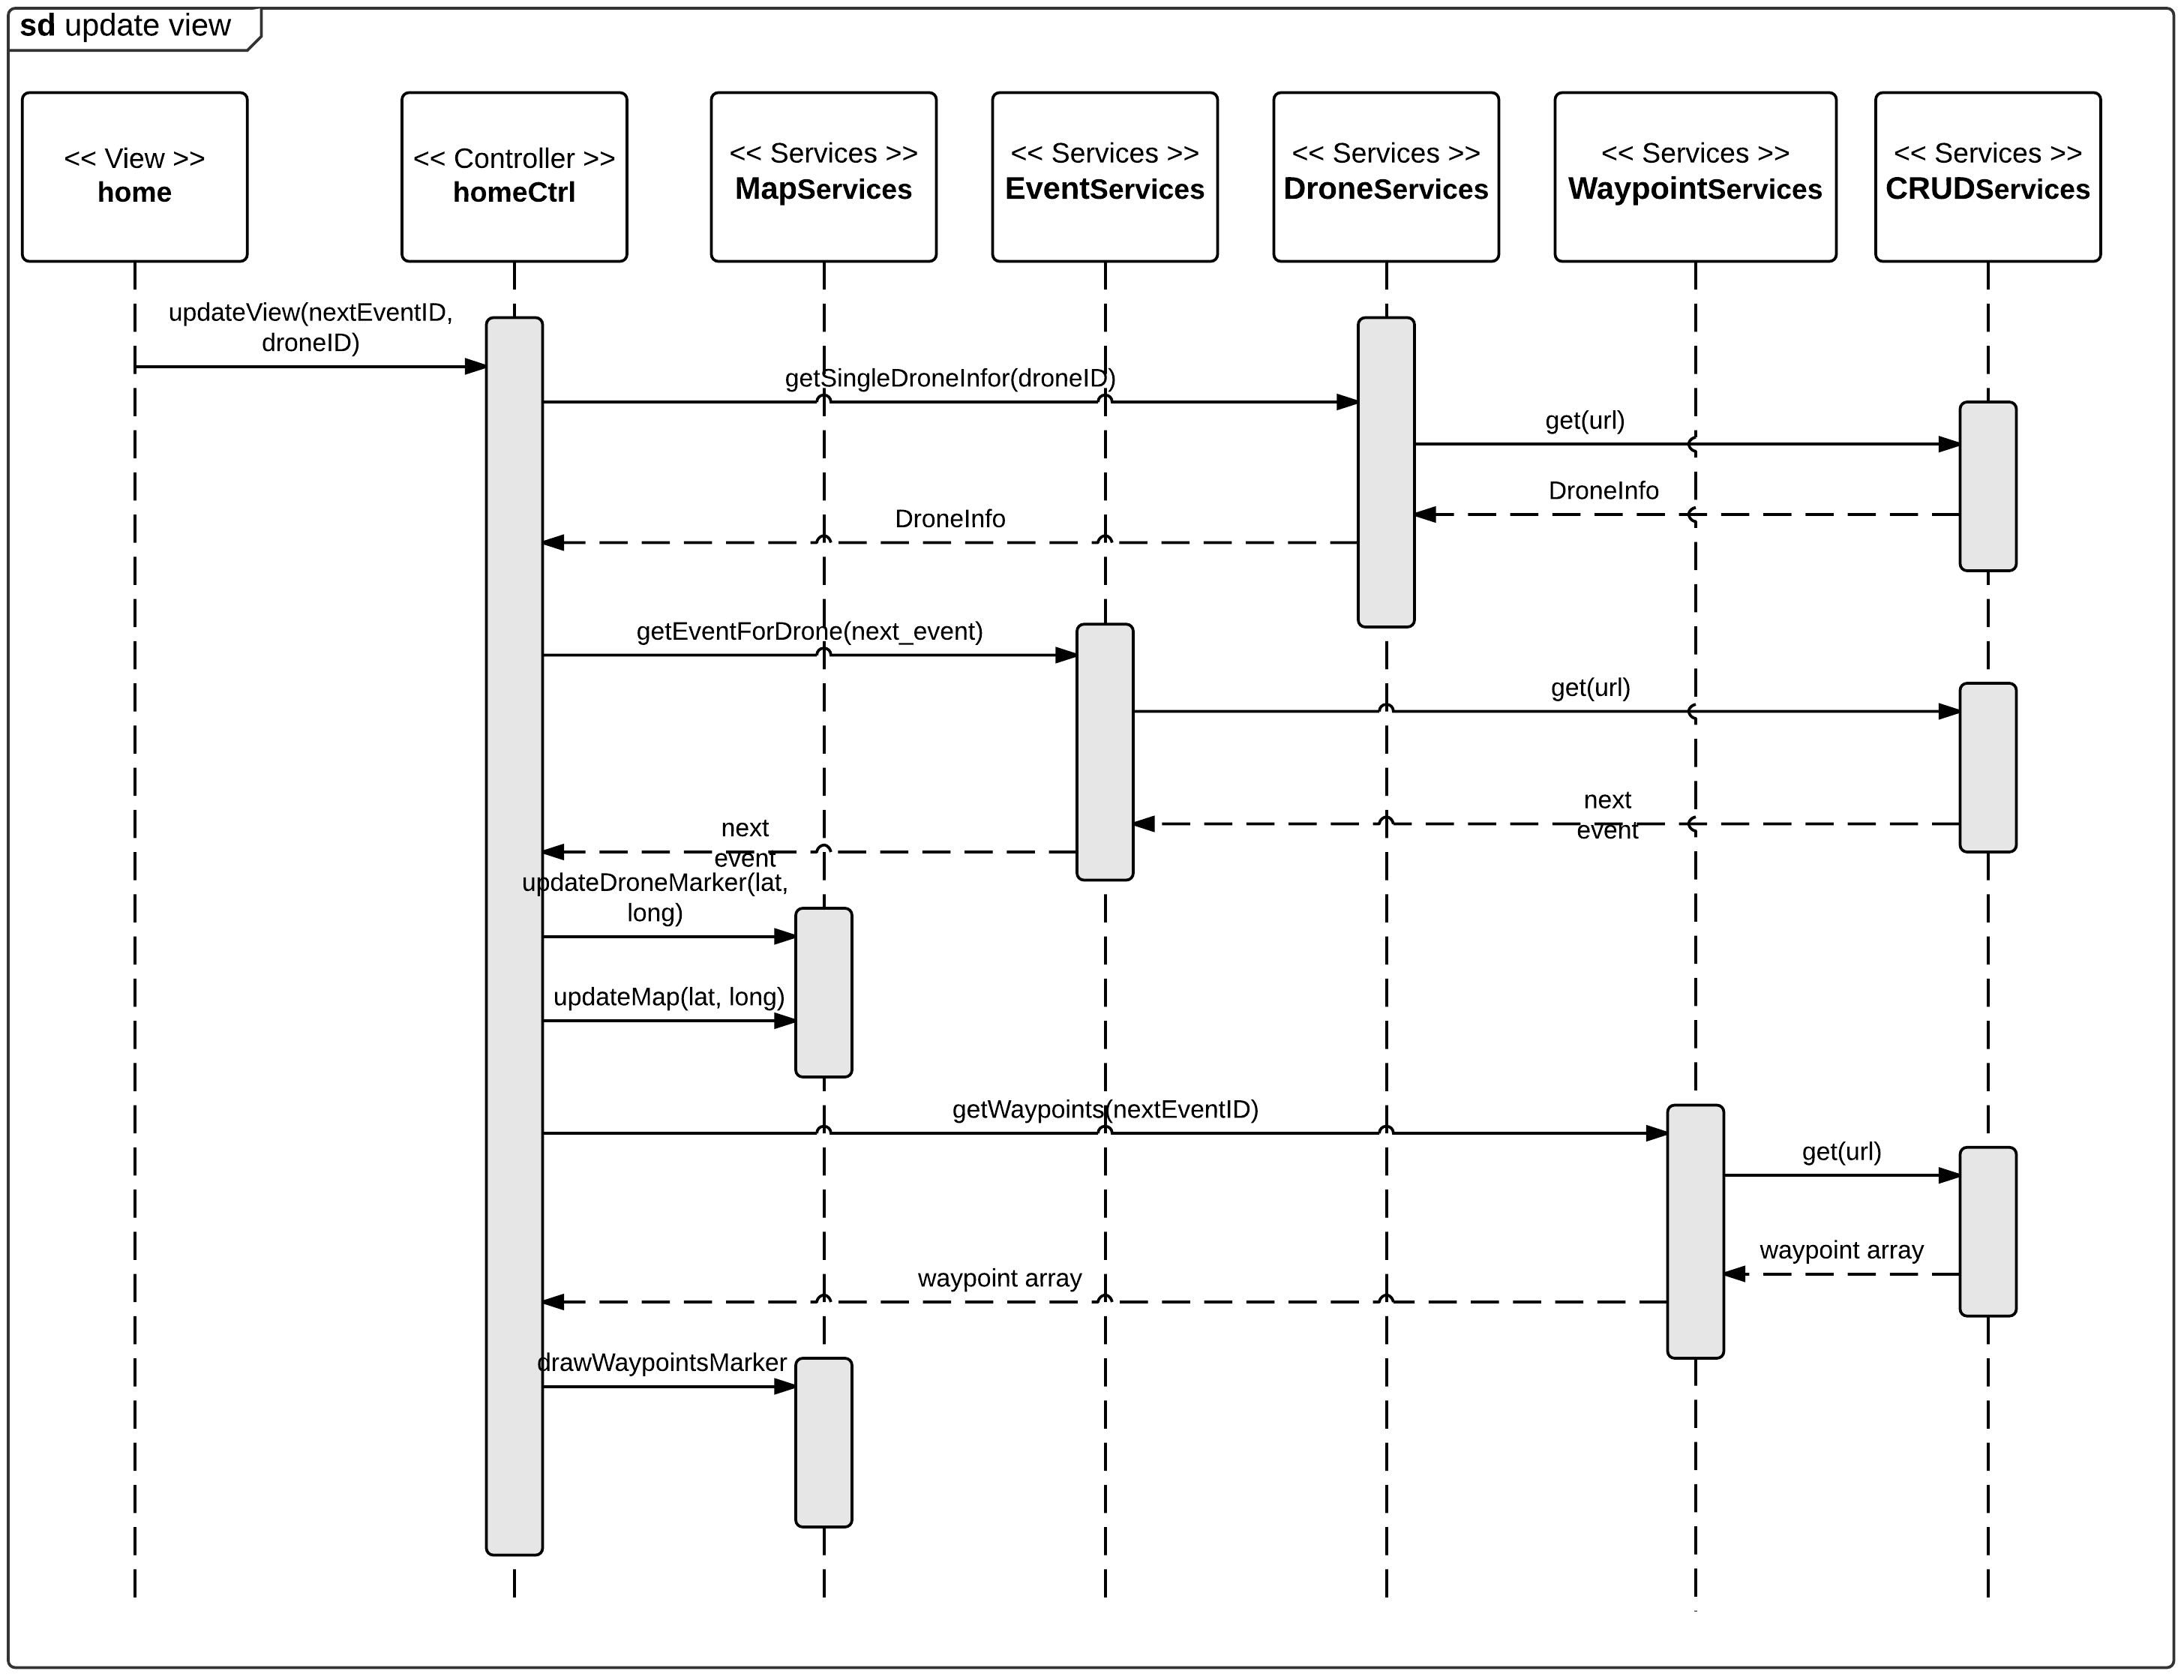
\includegraphics[width=1\textwidth]{Billeder/sekvens/sd_update_view.png}
	\caption{Sekvensdiagram opdater }
	\label{fig:update_view}
\end{figure}

\newpage
\subsubsection*{Klassediagram drone}

På figur \ref{fig:classDiagram_drone_underflyvning} ses klasse diagrammet for dronen. Det er klasserne der bruges af dronen, når den er flyve klar. På den følgende side er der en forklaring af klasserne og deres metoder. 

\begin{figure}[H]
	\centering
	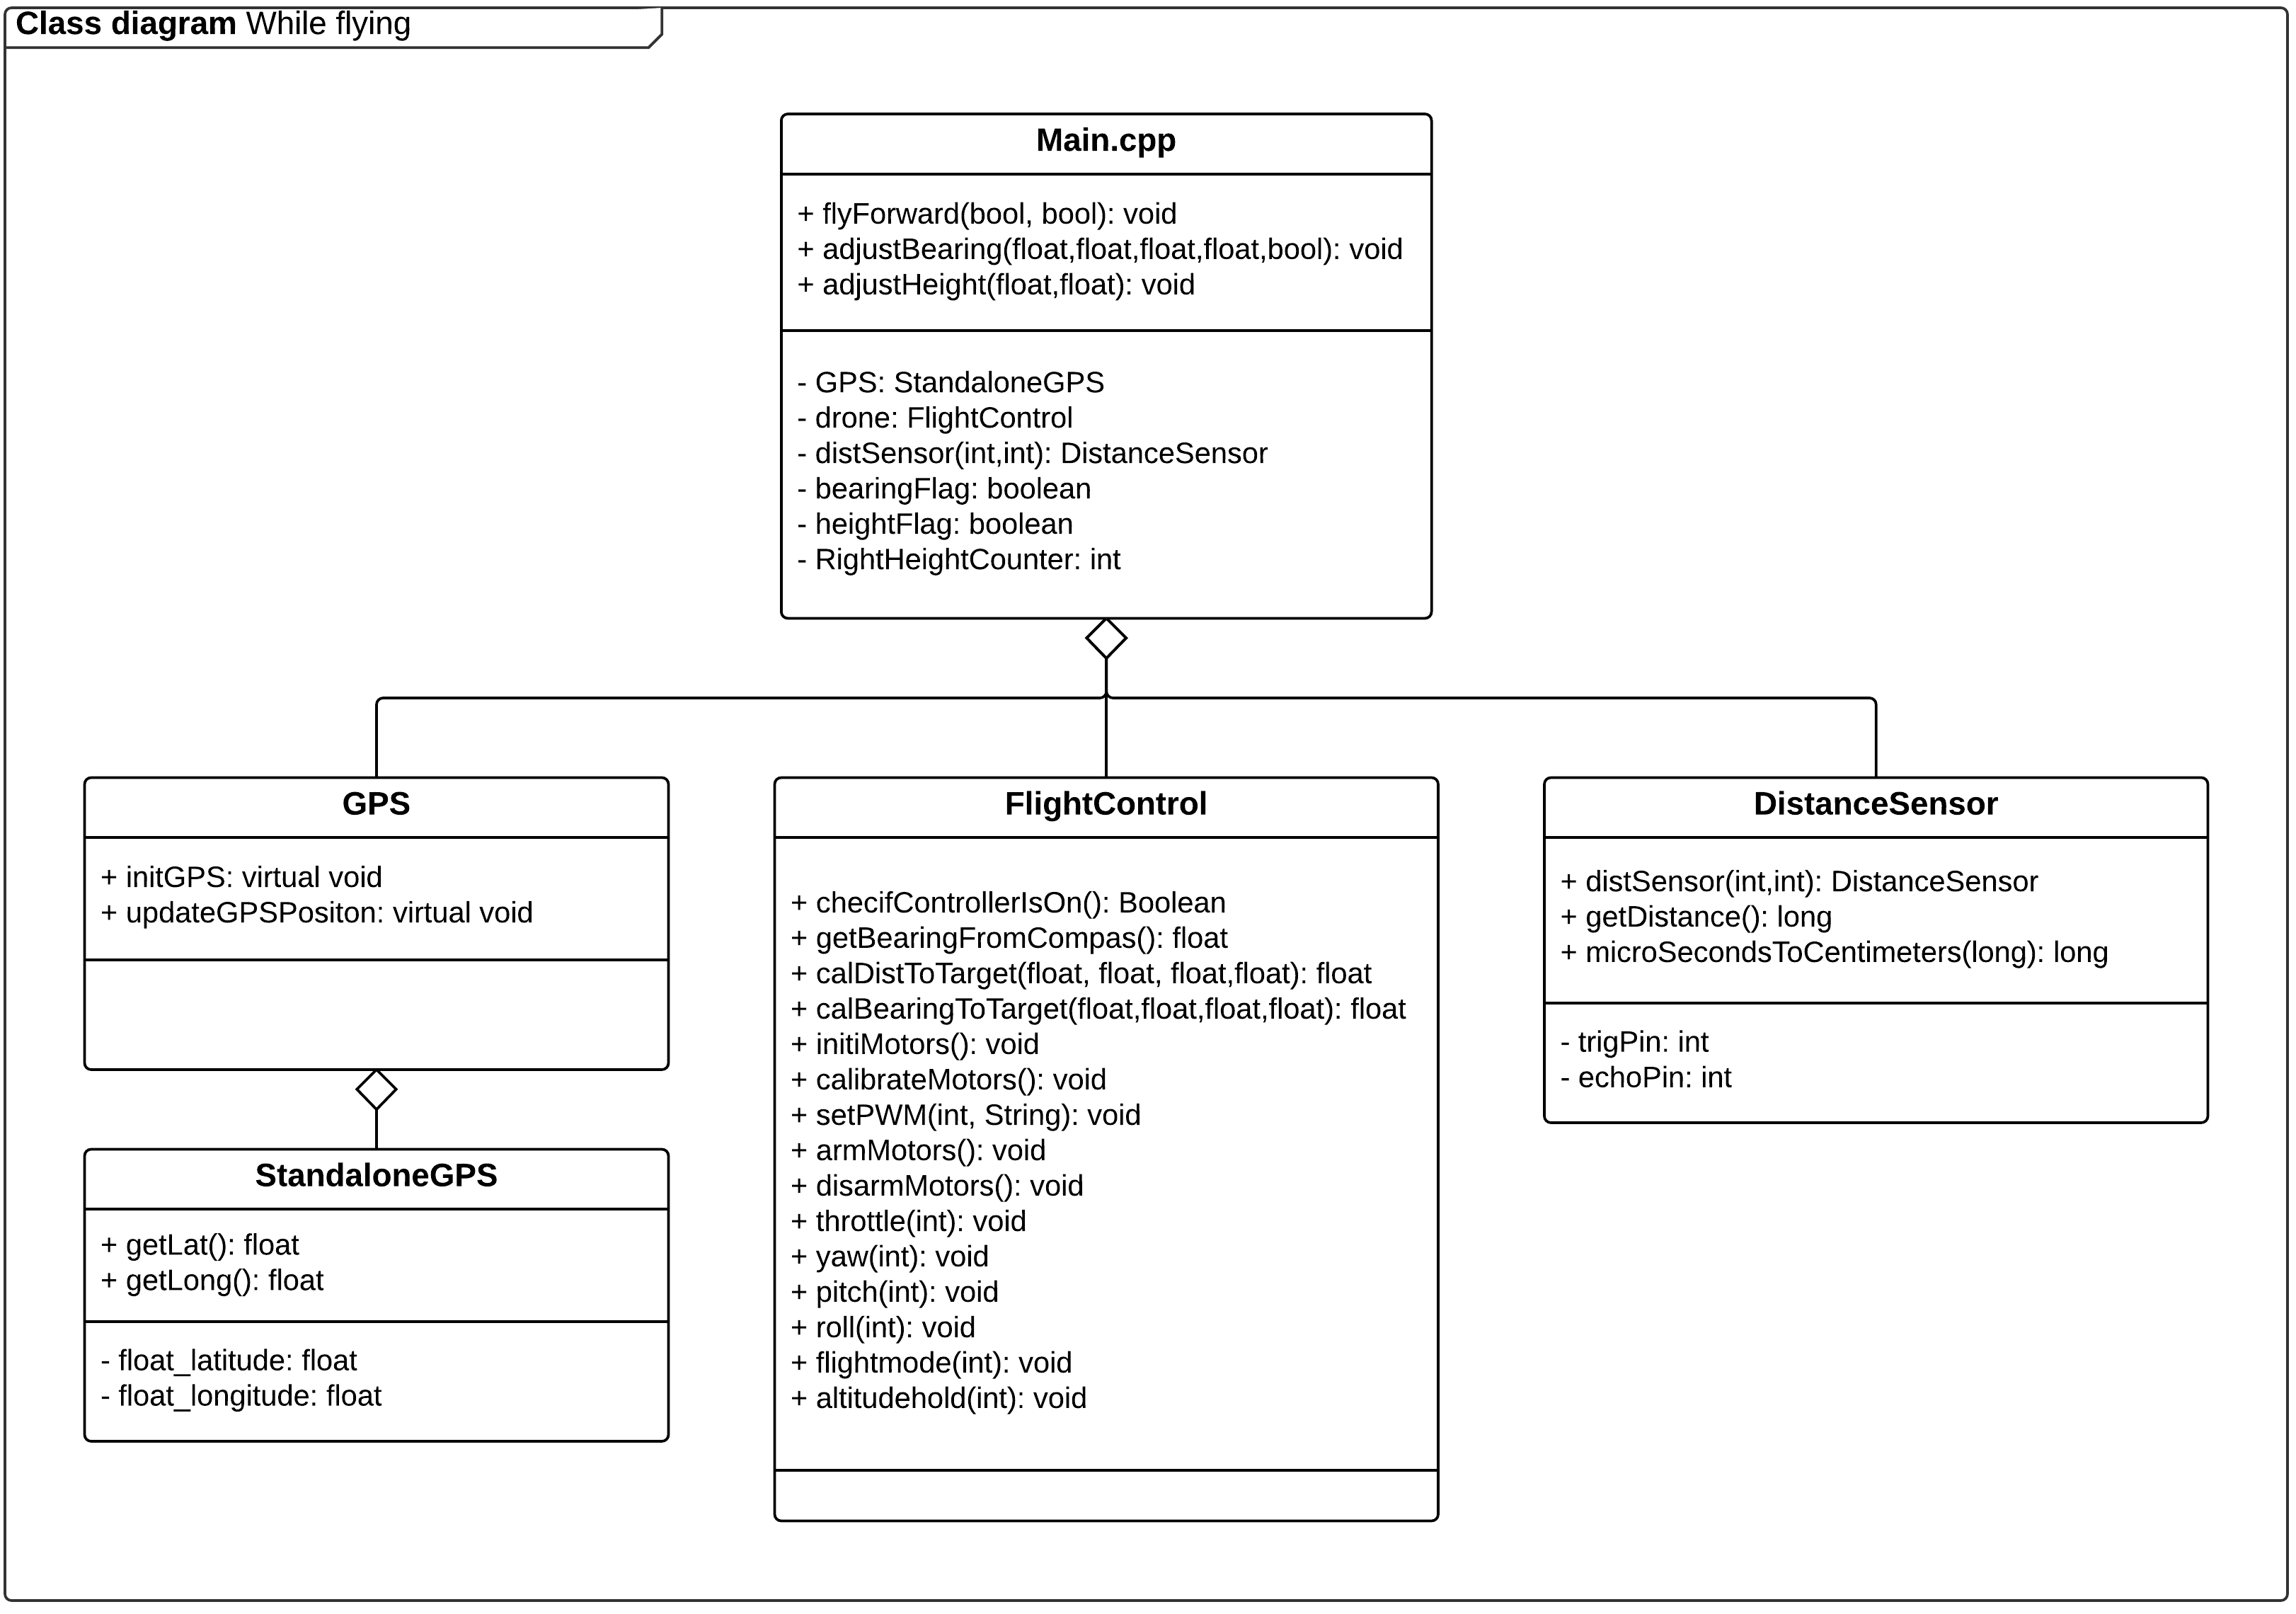
\includegraphics[width=1\textwidth]{Billeder/klasse_diagrammer/classdiagram_iteration2_fly.png}
	\vspace{0cm}
	\caption{Klassediagram drone}
	\label{fig:classDiagram_drone_underflyvning}
\end{figure}

\textbf{FlightControl} \\
Det er Flight Control klassen der har alt med styring af dronen at gøre, lige fra calibrering af motorerne til at hente data fra kompasset. 

\textbf{DistanceSensor} \\
DistanceSensor klassen bruges til at kontrollere de sensorer der er monteret på dronen. Her er det både sensorer til højdemåling og anti kollision. 

\textbf{GPS} \\
GPS klassen er implementeret som en abstract klasse, idet den ikke selv har nogle metoder den skal bruge, men med virtuelle metoder der sikrer at de implementeres i de afledte klasser. 
Init og updateGPSPosition er valgt til at være virtuelle klasser, hvilket gør at de skal implementeres uanset hvilken GPS der bruges. Klassen er lavet fordi der i udgangspunkt var mulighed for at bruge 3 forskellige slags GPS modes med 3G/GPS shieldet. 

\newpage
På Figur \ref{fig:classDiagram_3Gmodul} er der vist en udvidet klasse diagram for 3G modulet. På diagrammet vises de metoder og attributter der indgår i klasserne. 

\begin{figure}[H]
	\centering
	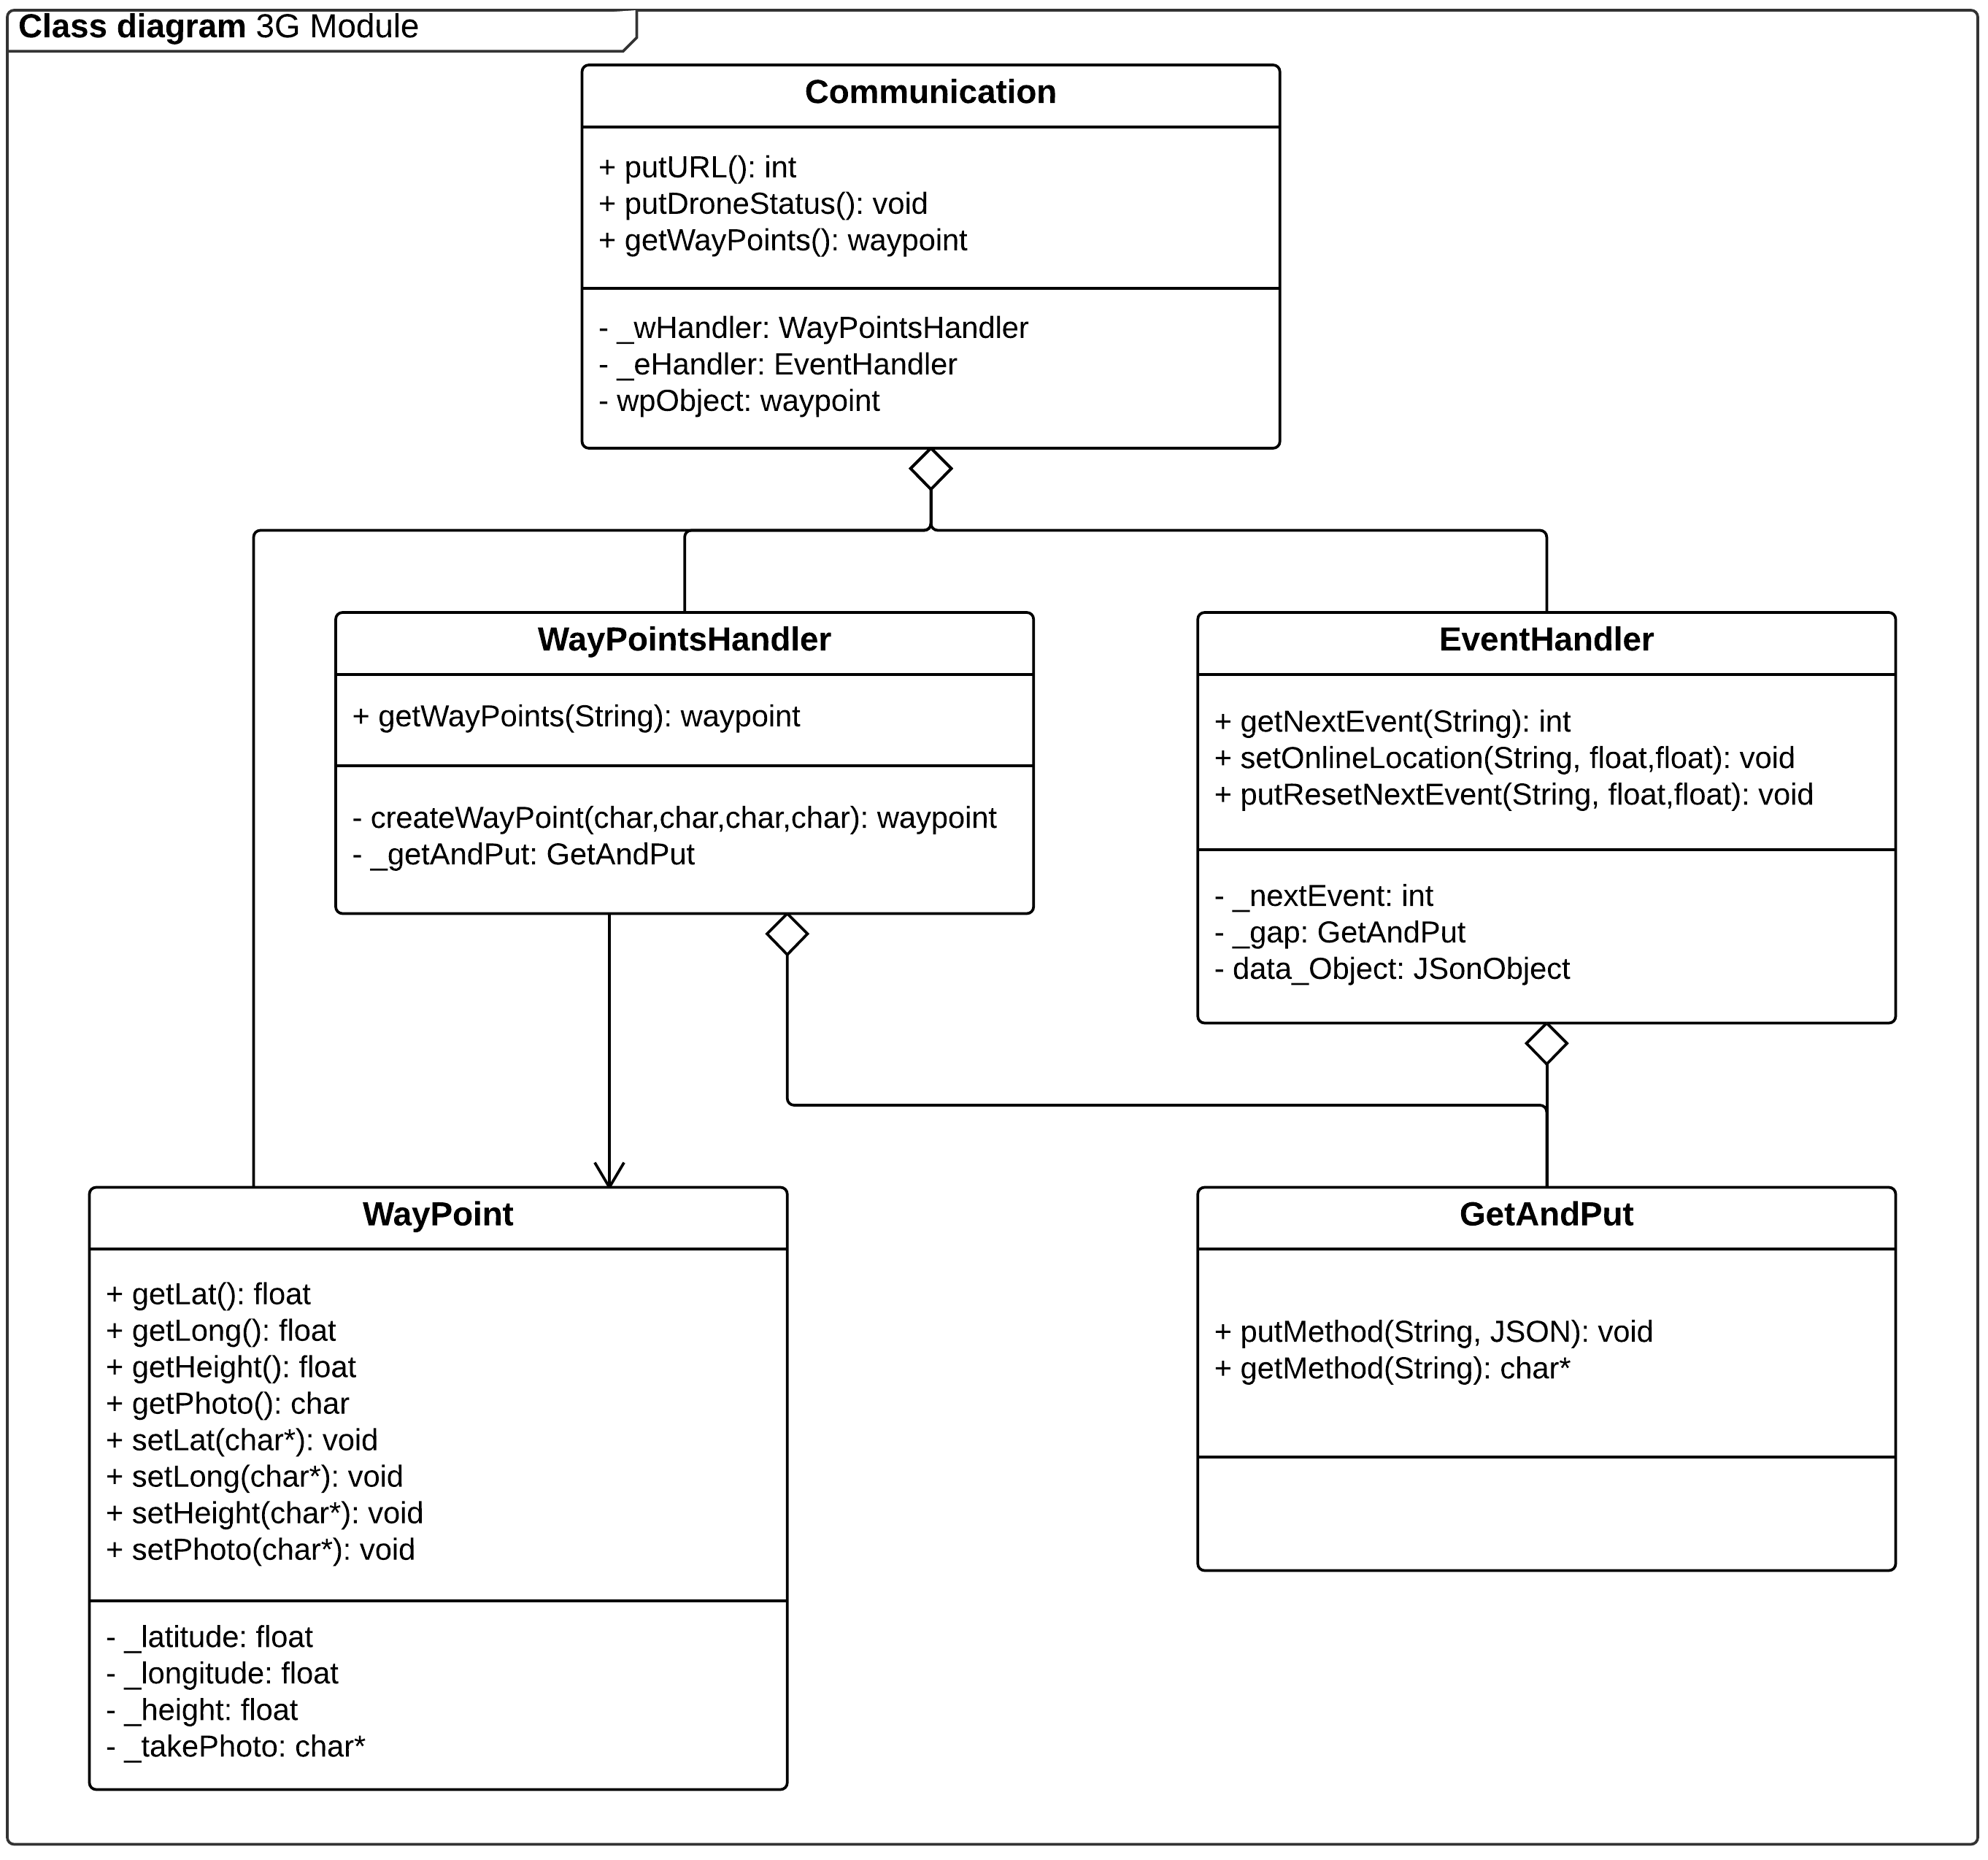
\includegraphics[width=1\textwidth]{Billeder/klasse_diagrammer/classdiagram_3gmodule.png}
	\vspace{0cm}
	\caption{Klassediagram 3G modul}
	\label{fig:classDiagram_3Gmodul}
\end{figure}


\textbf{GetAndPut} \\
GetAndPut klassen er den klasse der er tættest på hardwaren. Klassen indeholder de http metoder der bruges til kommunikation mellem dronen og serveren. 

\textbf{Communication} \\
Communication klassen er den øverste klasse og den håndterer sammen med andre klasser, alt der har med 3G at gøre.

\textbf{EventHandler} \\
EventHandleren er den klasse der håndterer Events. EventHandleren er bindeledet mellem communication- og GetAndPut klassen. EventHandleren sorterer eventID'et fra de data den modtager og returnerer værdien til communication klassen.

\newpage

\textbf{WayPointsHandler} \\
WayPointsHandler klassen er den klasse der håndterer de waypoints der hentes ned fra serveren. Klassen tager de waypoints den får fra serveren og gør dem tilgængeligt for resten af systemet. WayPointsHandleren bruger set metoderne i WayPoint klassen.

\textbf{WayPoint} \\
WayPoint klassen bruges til at kunne hente de forskellige waypoints ud af arrayet.  


\subsubsection*{Klassediagram webapplikation}
\vspace{-0.1cm}
På figur \ref{fig:classDiagram_home} ses klasse diagrammet tilhørende iteration to for websitet. Funktionaliteten er blevet udvidet med overblik over droner i systemet og deres status. Mulighed for at oprette events til den ønskede drone. 
\begin{figure}[H]
	\centering
	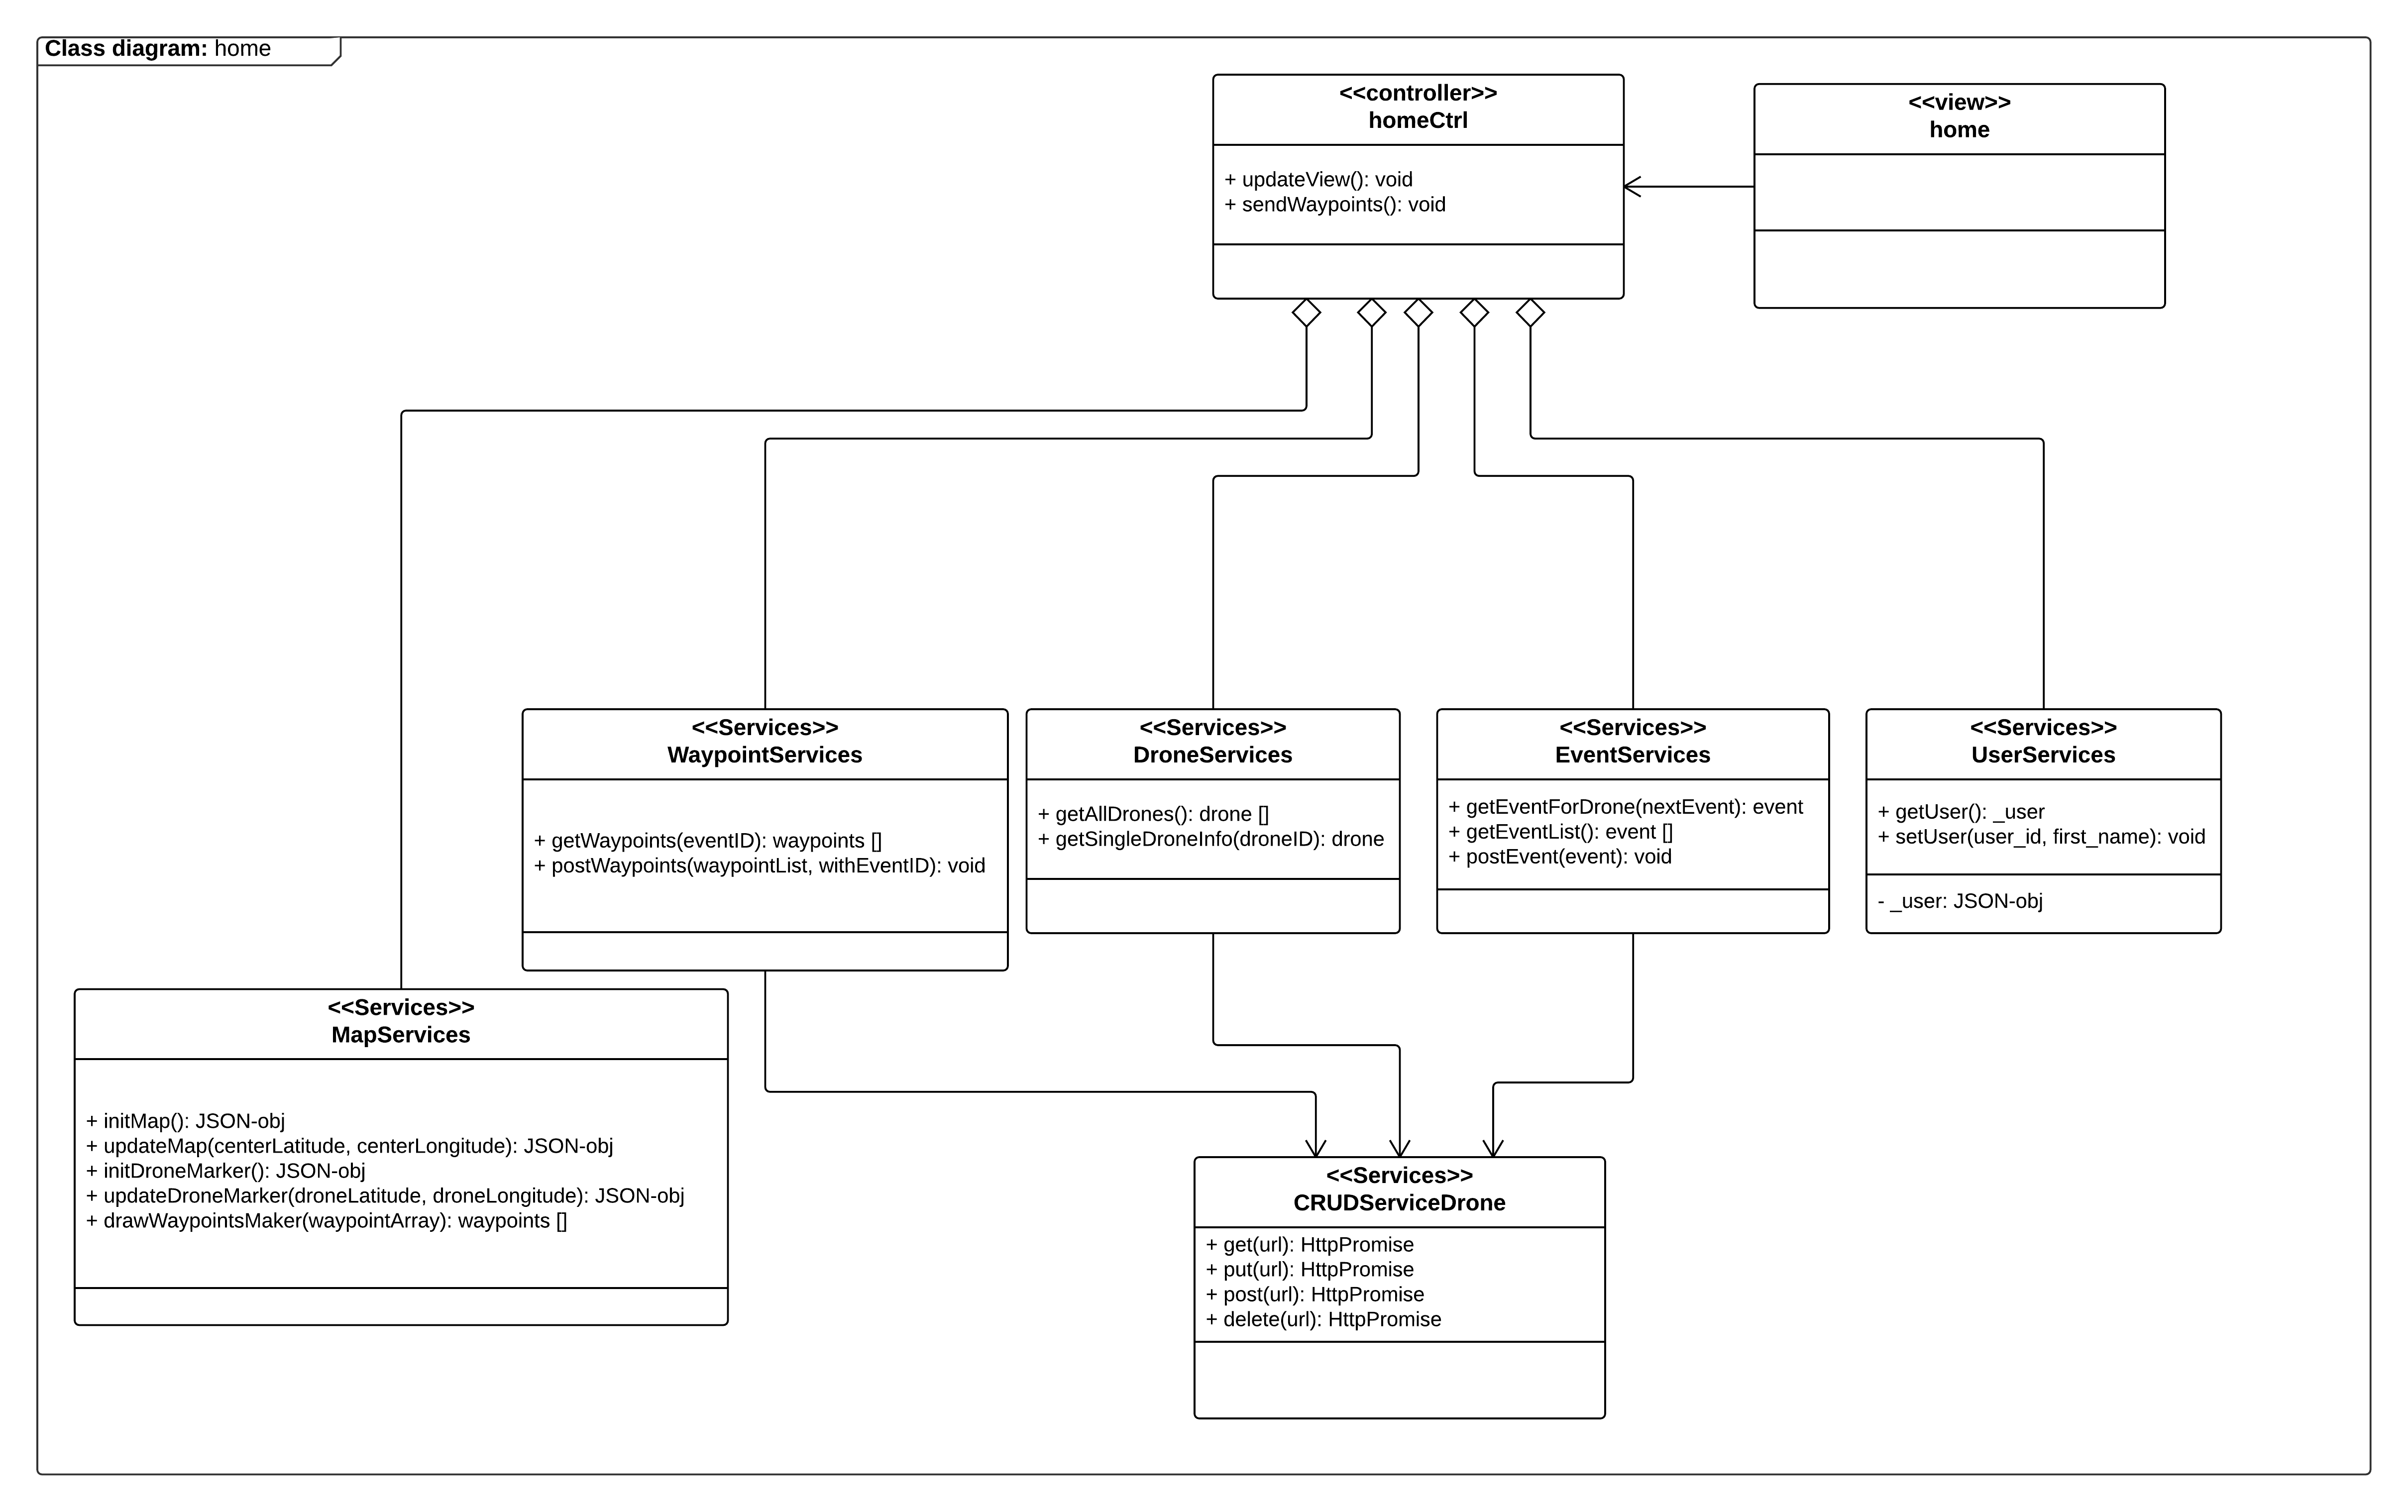
\includegraphics[width=1.\textwidth]{Billeder/klasse_diagrammer/home_class_diagram.png}
	\vspace{-0.5cm}
	\caption{Klassediagram home}
	\label{fig:classDiagram_home}
\end{figure}

\textbf{home}
Denne klasse er view'et tilhørende iteration to. Denne klasse sammen med homeCtrl skaber det endelig view som brugeren ser i sin browser når han besøger siden.

\textbf{homeCtrl}
HomeCtrl klassen er controller klassen til iteration to. Det er den eneste klasse der har direkte forbindelse til view'et, homeCtrl klassen deler også hukommelse med view'et igennem two-way-binding med scopes.

\textbf{DroneServices}
Denne klasse indeholder logikken om drone håndteringen. Den har ansvaret for at hente informationer omkring droner fra serveren via CRUDServiceDrone klassen.

\textbf{WaypointServices}
Denne klasse indeholder logikken om waypoint håndtering. Denne klasse henter henter waypoints tilhørende et event til controller klassen. Klassen bliver også brugt til at sende waypoints til serveren via CRUDServiceDrone klassen.

\textbf{EventServices}
Denne klasse indeholder logikken om event håndtering. Klassen bruges til at hente en event liste, et enkelt event for en givet drone og sende et nyoprettet event til serveren via CRUDServiceDrone klassen.

\textbf{MapServices}
Denne klasse indeholder logikken om map håndtering. Klassen bruges til at opdatere kortet i view'et, tegne waypoints og dronen på kortet.

\textbf{CRUDServicesDrone}
Denne klasse fungere som bindeled imellem server og webapplikation. Klassen indeholder alt logikken omkring kommunikation til serveren, alle der vil kommunikere med serveren i systemet skal benytte sig af denne klasse. Igennem denne service er det muligt at hente, opdater og poste data til serveren.

\textbf{UserServices}
Denne klasse blev oprettet i iteration et og bruges til at gemme information omkring hvilke bruger der er logget ind i systemet.

%\newpage
%\subsection{Iteration \#3}
I iteration 3 arbejdes med blokke som skal håndterer hvordan der tages billeder, forsendelse af billeder og billede visning. Der monteres kamera på dronen, så den under flyvning kan tage billeder ved de GPS lokationer som bruger har defineret i flyveopsætningen. Alle billeder der tages under flyvning sendes via mobilnet fra dronen til server. Websiden henter automatisk de seneste billeder fra serveren og gør disse tilgængelige for bruger. Hvordan systemet er tiltænkt at bruges beskrives i user story nedenfor:

\subsubsection*{User story}
Under flyvning tager dronen billeder som sendes via 3G/GPS modulet til serveren. Websiden kontrollerer løbende hvilke billeder der er findes på serveren og gør disse tilgængelig for bruger. Login er påkrævet før bruger kan få lov at se billeder fra forskellige flyvninger. Efter succesfuld login på websiden vælger bruger historik og vises information fra tidligere flyvninger. 

%kommentar
\begin{figure}[H]
	\centering
	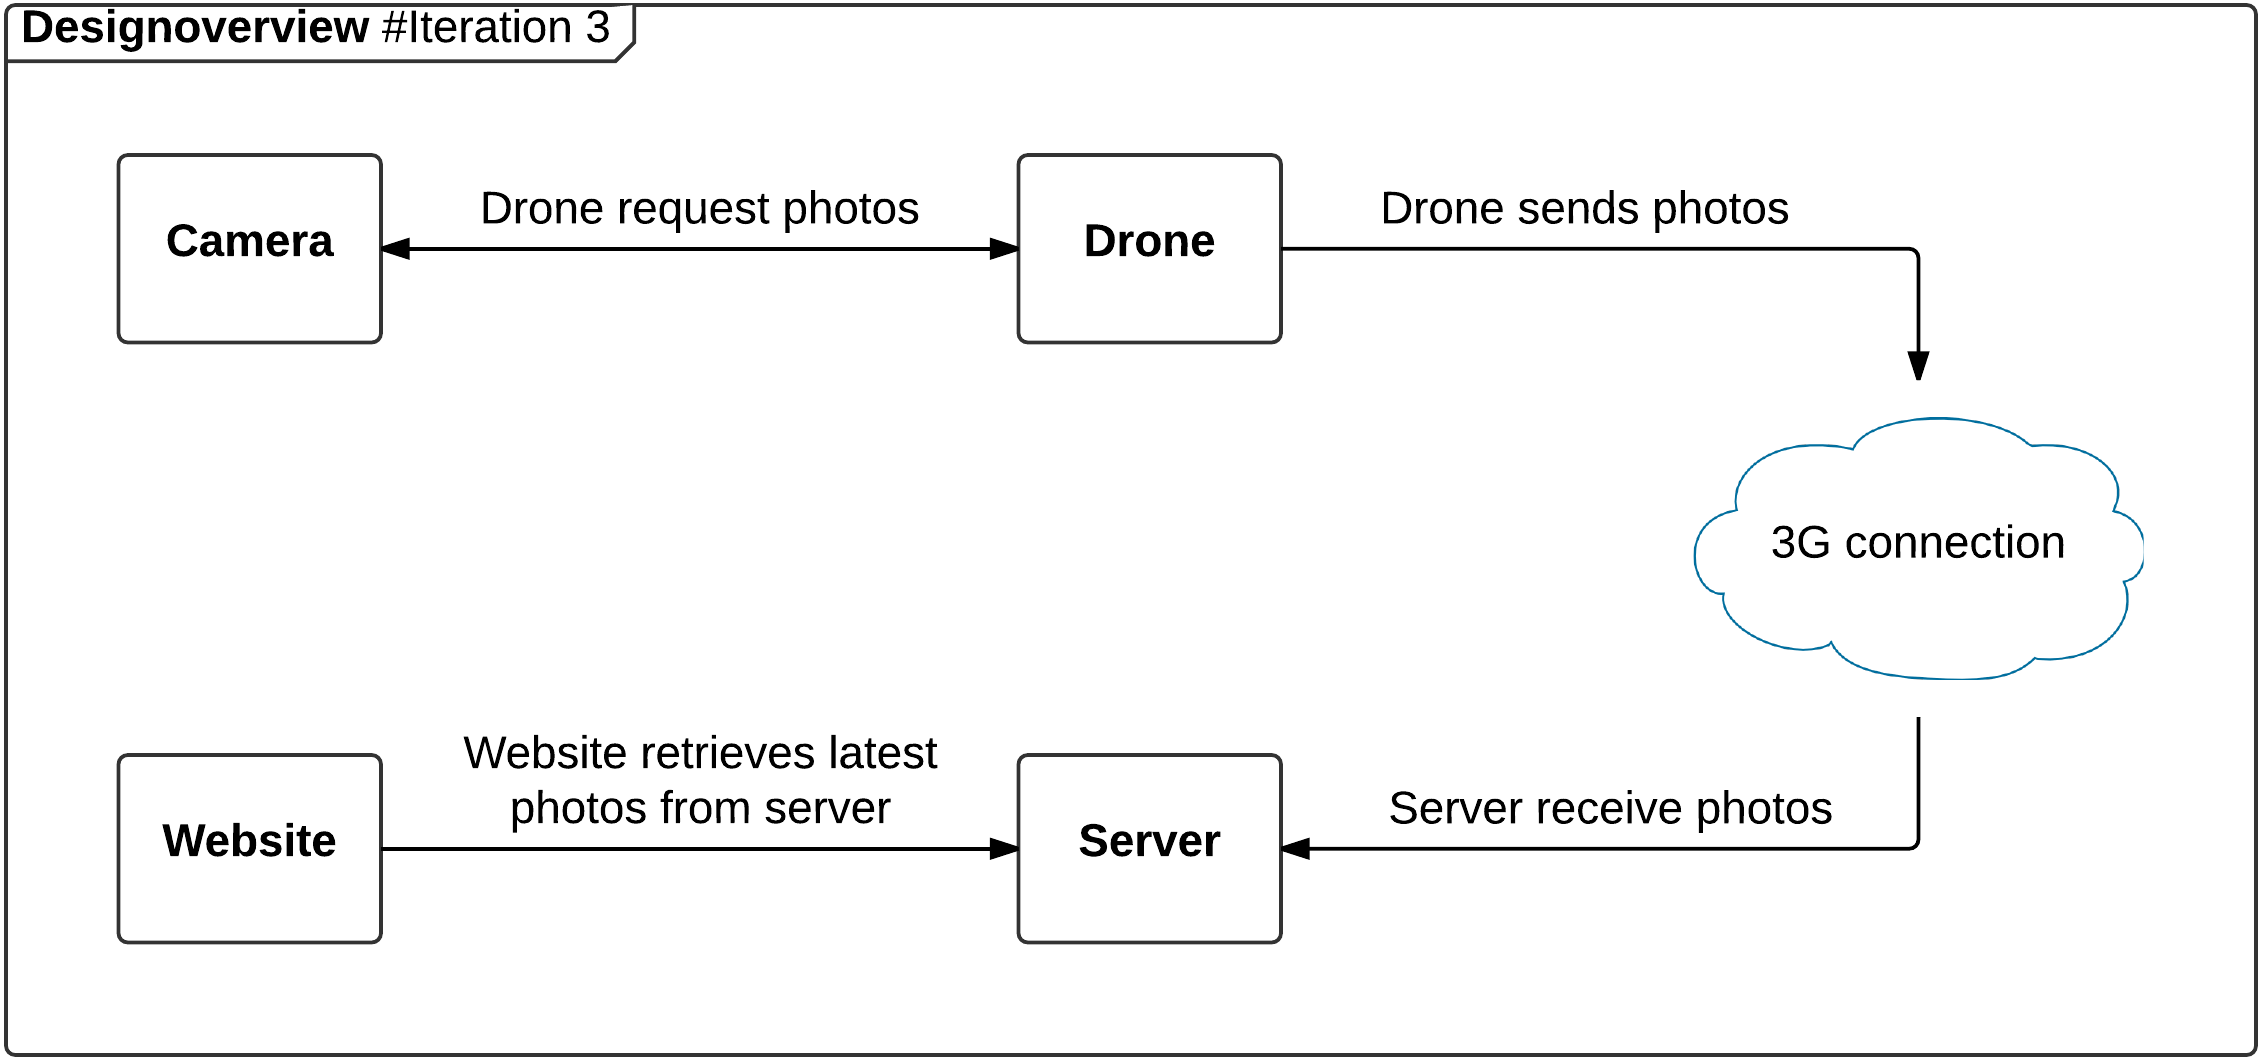
\includegraphics[width=1\textwidth]{Billeder/design_overview/design_overview_iteration3.png}
	\vspace{-.5cm}
	\caption{Designoverview \#iteration 3}
	\label{fig:design_overview_UC1}
\end{figure}
\newpage

\newpage
\subsubsection*{Pakkediagram drone}
I dette afsnit vises pakkediagram tilhørende drone. Hver pakke i pakkediagrammet består af en eller flere klasser, der med stort samspil udfører opgaver indenfor et fælles ansvarsområde. 
På hver pakke findes en lille beskrivelse, der tydeliggør pakkens ansvarsområde. De dele af pakkerne der er gråskraveret, er funktionalitet udarbejdet i tidligere iteration.


\begin{figure}[H]
	\centering
	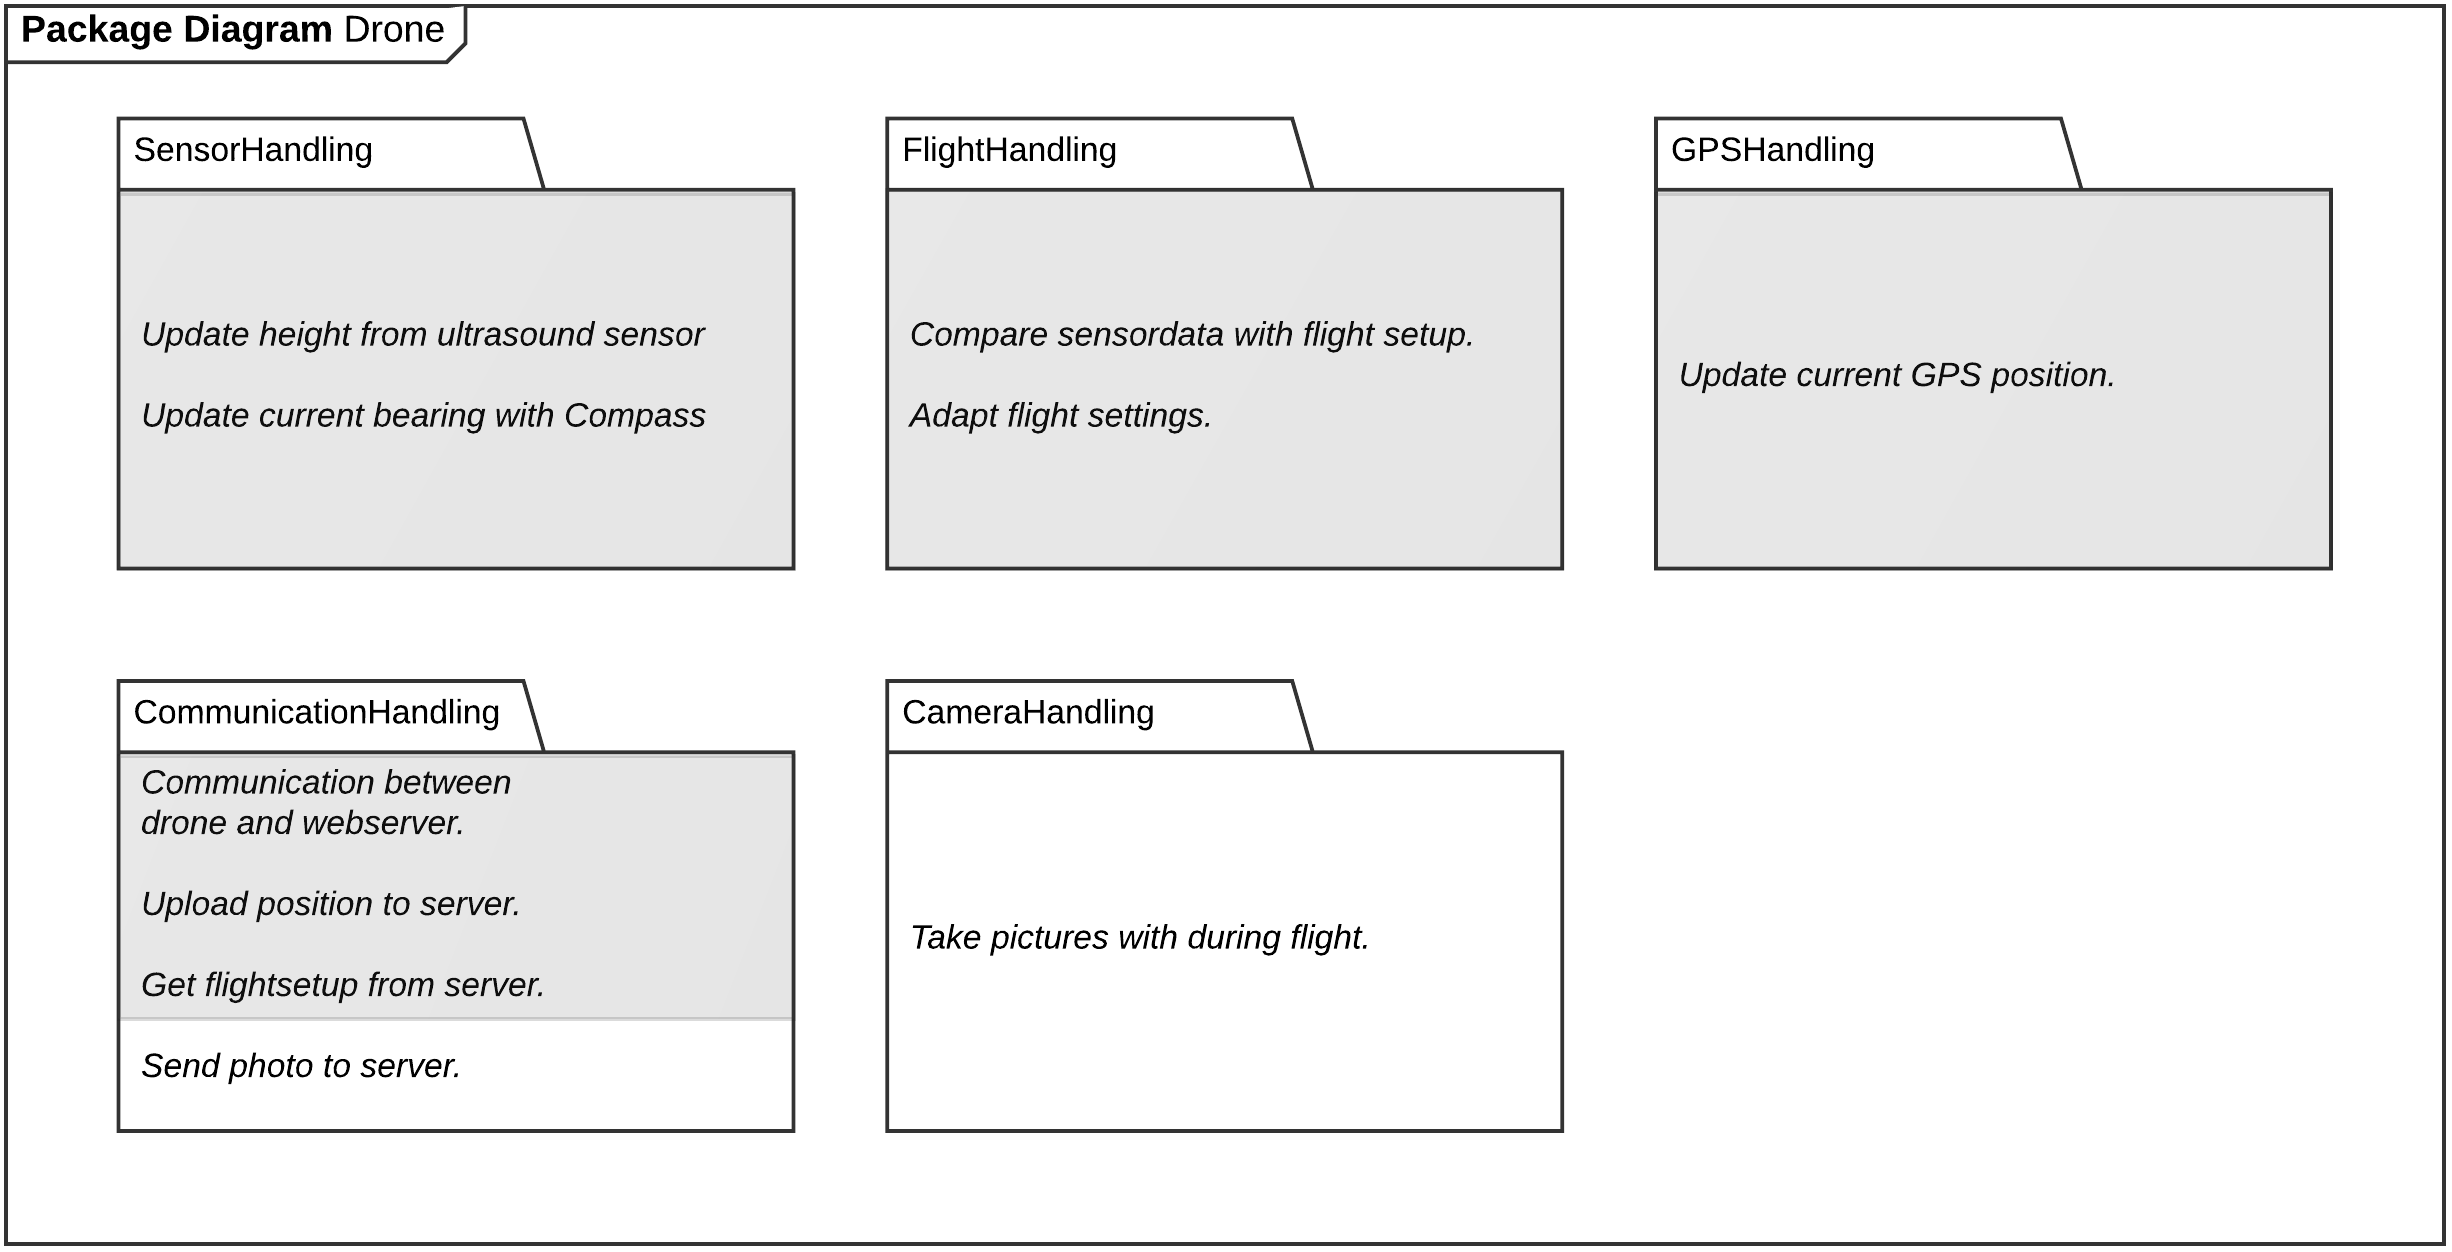
\includegraphics[width=1\textwidth]{Billeder/pakke_diagrammer/iteration3_drone.png}
	\vspace{-0.5cm}
	\caption{Pakkediagram drone}
	\label{fig:iteration2_pakke_diagram_drone}
\end{figure}

\textbf{SensorHandling}\\
Pakken er ansvarlig for indsamling af sensor data. I denne iteration skal pakken bruges til aflæsning af højdemåler og kompasset på flight control boardet. 

\textbf{FlightHandling}\\
Pakkens ansvar er kontrol og styring af drone under flyvning. Ved sammenligning af sensor data og data fra flyveopsætning tilpasses flyvehøjde, orientering mm

\textbf{GPSHandling}\\
Pakkens ansvar er håndtering af GPS. Dels er pakken ansvarlig for opstart og initiering af GPS, og desuden bruges pakken hver gang dronens nuværende GPS position skal opdateres.

\textbf{CommunicationHandling}\\
Pakkens ansvar er kommunikation imellem drone og server. Efter denne iteration skal dronen kunne hente flyveopsætninger fra server, sende sin nuværende GPS position til server og sende billeder til server.

\textbf{CameraHandling}\\
Pakkens ansvar er håndtering af kamera. Pakken bruges til at starte, initierer, bruge og slukke kameraet.


\newpage
\subsubsection*{Pakkediagram webapplikation}
I dette afsnit vises pakkediagram tilhørende webapplikation. Hver pakke i pakkediagrammet består af en eller flere klasser, der med stort samspil udfører opgaver indenfor et fælles ansvarsområde. 
På hver pakke findes en lille beskrivelse, der tydeliggør pakkens ansvarsområde. De dele af pakkerne der er gråskraveret, er funktionalitet udarbejdet i tidligere iteration. 

\begin{figure}[H]
	\centering
	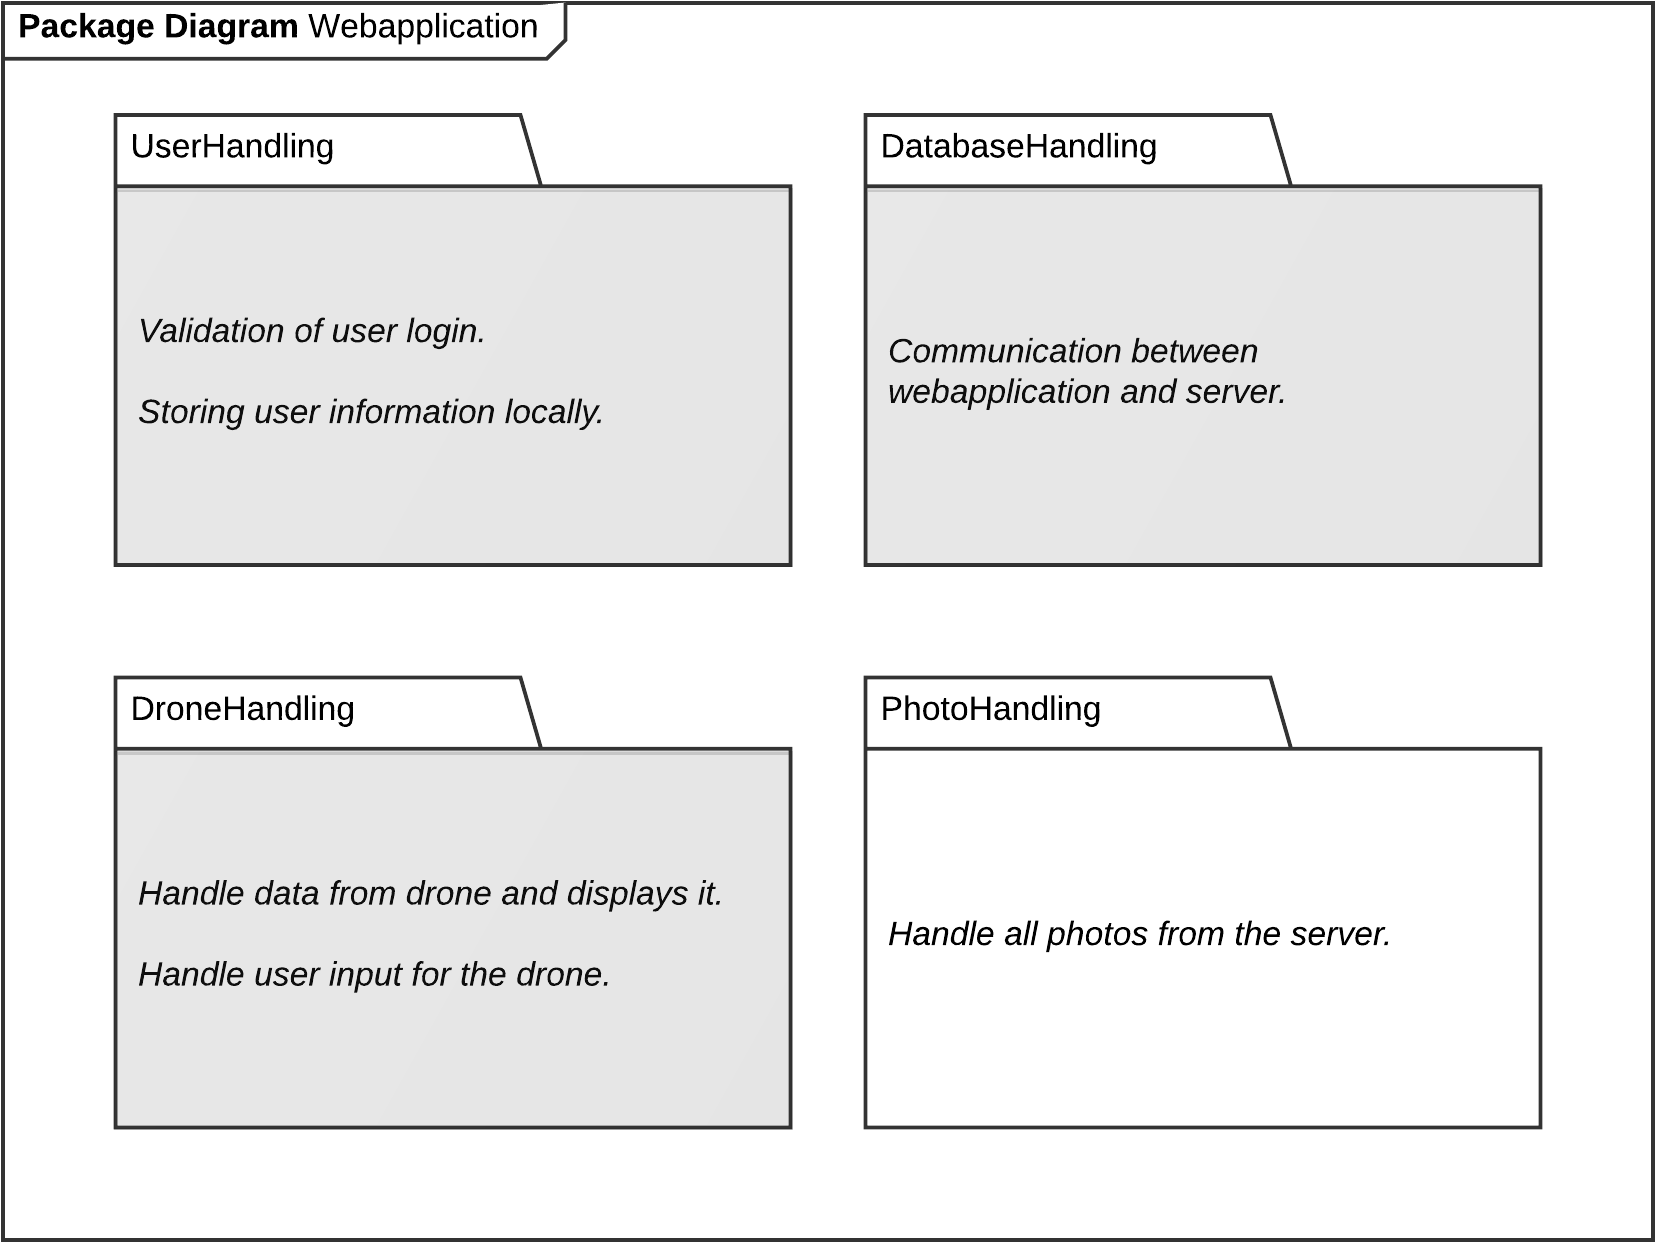
\includegraphics[width=1\textwidth]{Billeder/pakke_diagrammer/iteration3_server.png}
	\vspace{-0.5cm}
	\caption{Pakkediagram webapplikation}
	\label{fig:iteration3_pakke_diagram_webapplikation}
\end{figure}

\textbf{UserHandling}\\
Pakkens ansvar er validering af login/log ud på websitet. Pakken har også ansvaret for at hente og gemme data om den pågældende bruger.

\textbf{DatabaseHandling}\\
Pakkens ansvar er kommunikation imellem databasen og serveren. 

\textbf{DroneHandling}\\
Pakkens ansvar er alt data vedrørende dronen, så som håndteringen af events, waypoints og div droner.

\textbf{PhotoHandling}\\
Pakkens ansvar er at håndtere de billeder dronen har taget under flyvning og præsentere dem for brugeren.

\newpage

\subsubsection*{Sekvens diagram}
\vspace{-0.3cm}
På sekvensdiagrammet på figur \ref{fig:Sekvens_diagram_iteration3}, vises hvilke klasser der indgår og bruges i tredje iteration. På sekvensdiagrammet vises det hvordan kamera delen af 3G/GPS modulet håndteres og hvordan ny tagede billeder sendes med post request til serveren. 

\vspace{-0.2cm}
%kommentar
\begin{figure}[H]
	\centering
	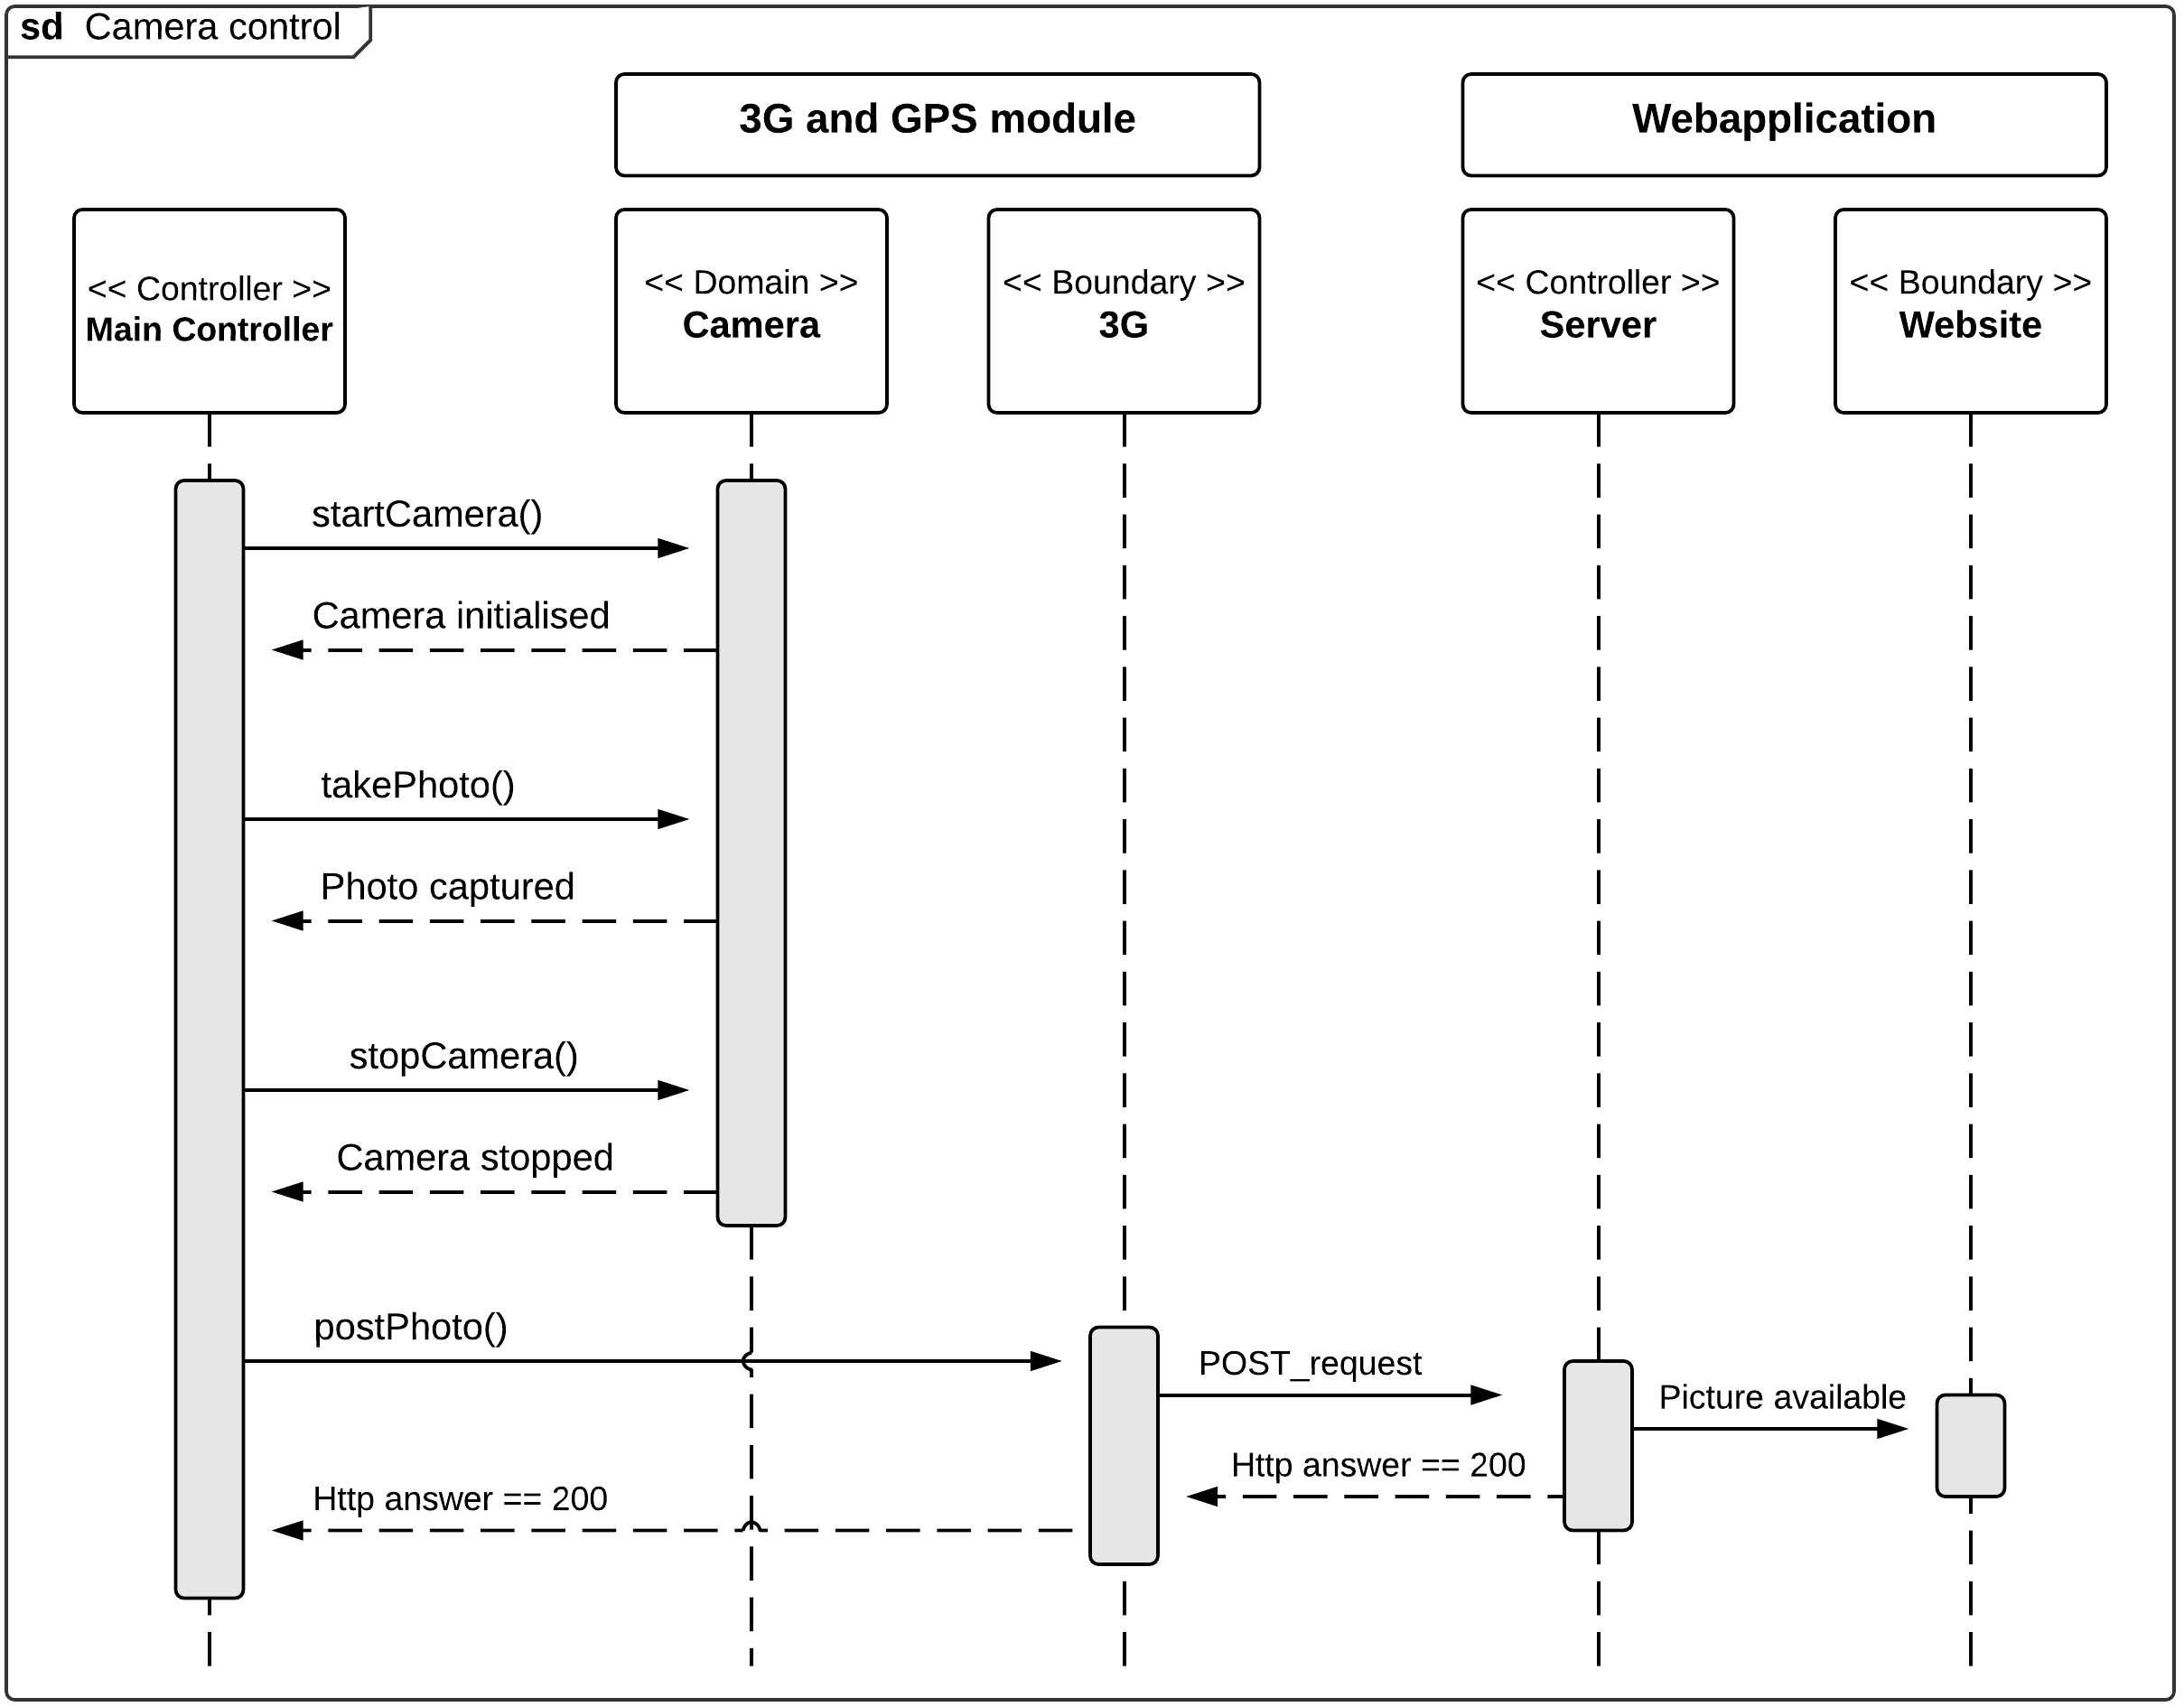
\includegraphics[width=1\textwidth]{Billeder/sekvens/sekvens_iteration3}
	\caption{Sekvens diagram \#iteration 3}
	\label{fig:Sekvens_diagram_iteration3}
\end{figure}
\vspace{-0.2cm}

\newpage

\subsubsection*{Klassediagram drone}

Figur \ref{fig:classDiagram_iteration3} vises et klassediagram tilhørende iteration 3. Klassediagrammet viser foruden main.cpp filen iteration 3's eneste centrale klasse og dens tilhørende metode. 

%kommentar
\begin{figure}[H]
	\centering
	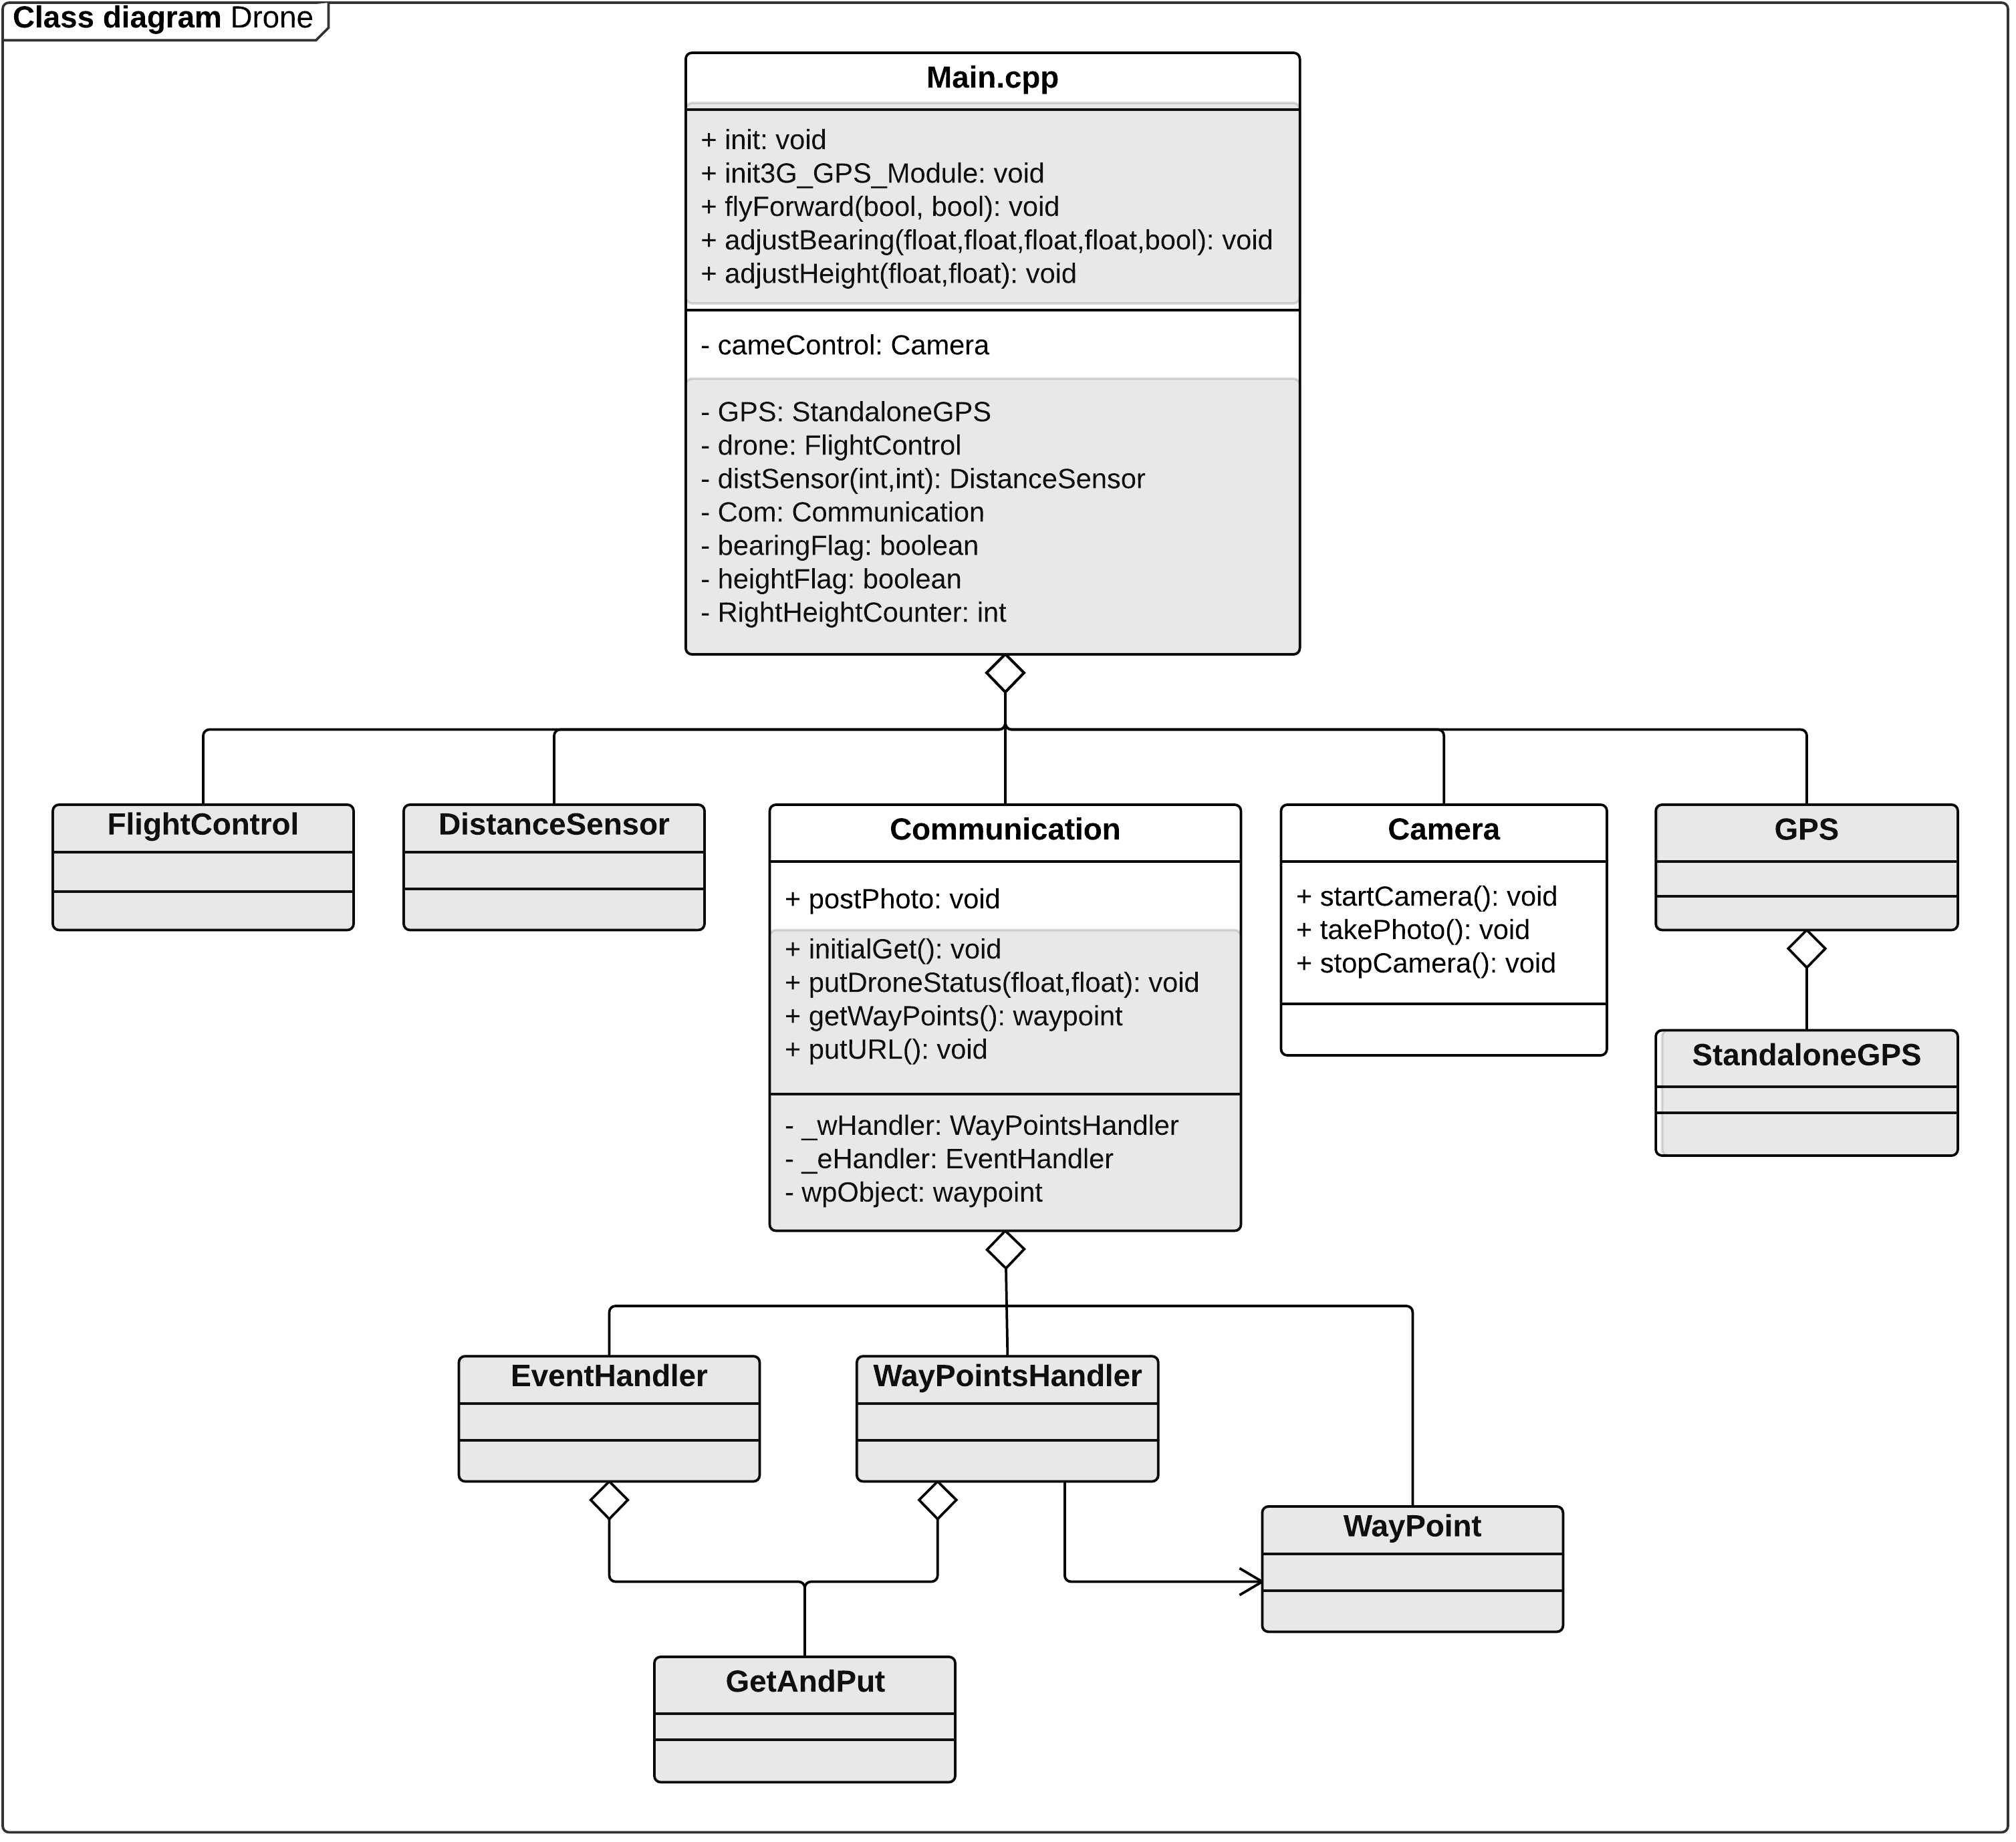
\includegraphics[width=1\textwidth]{Billeder/klasse_diagrammer/classdiagram_iteration3_drone.png}
	\vspace{-0.5cm}
	\caption{Klassediagram \#iteration 3}
	\label{fig:classDiagram_iteration3}
\end{figure}

\textbf{Main.cpp} \\
Main.cpp filen bruges til at oprette objekter af de Anti collision klassen og til at kalde dens tilhørende funktioner.

\textbf{Camera} \\
Klassen eneste funktion er at kontrollere afstanden til eventuelle objekter foran dronen. 


\newpage

\subsubsection*{Klassediagram webapplikation}

Figur \ref{fig:classDiagram_iteration3} vises klassediagrammet tilhørende iteration 3 for webapplikationen. 

%kommentar
\begin{figure}[H]
	\centering
	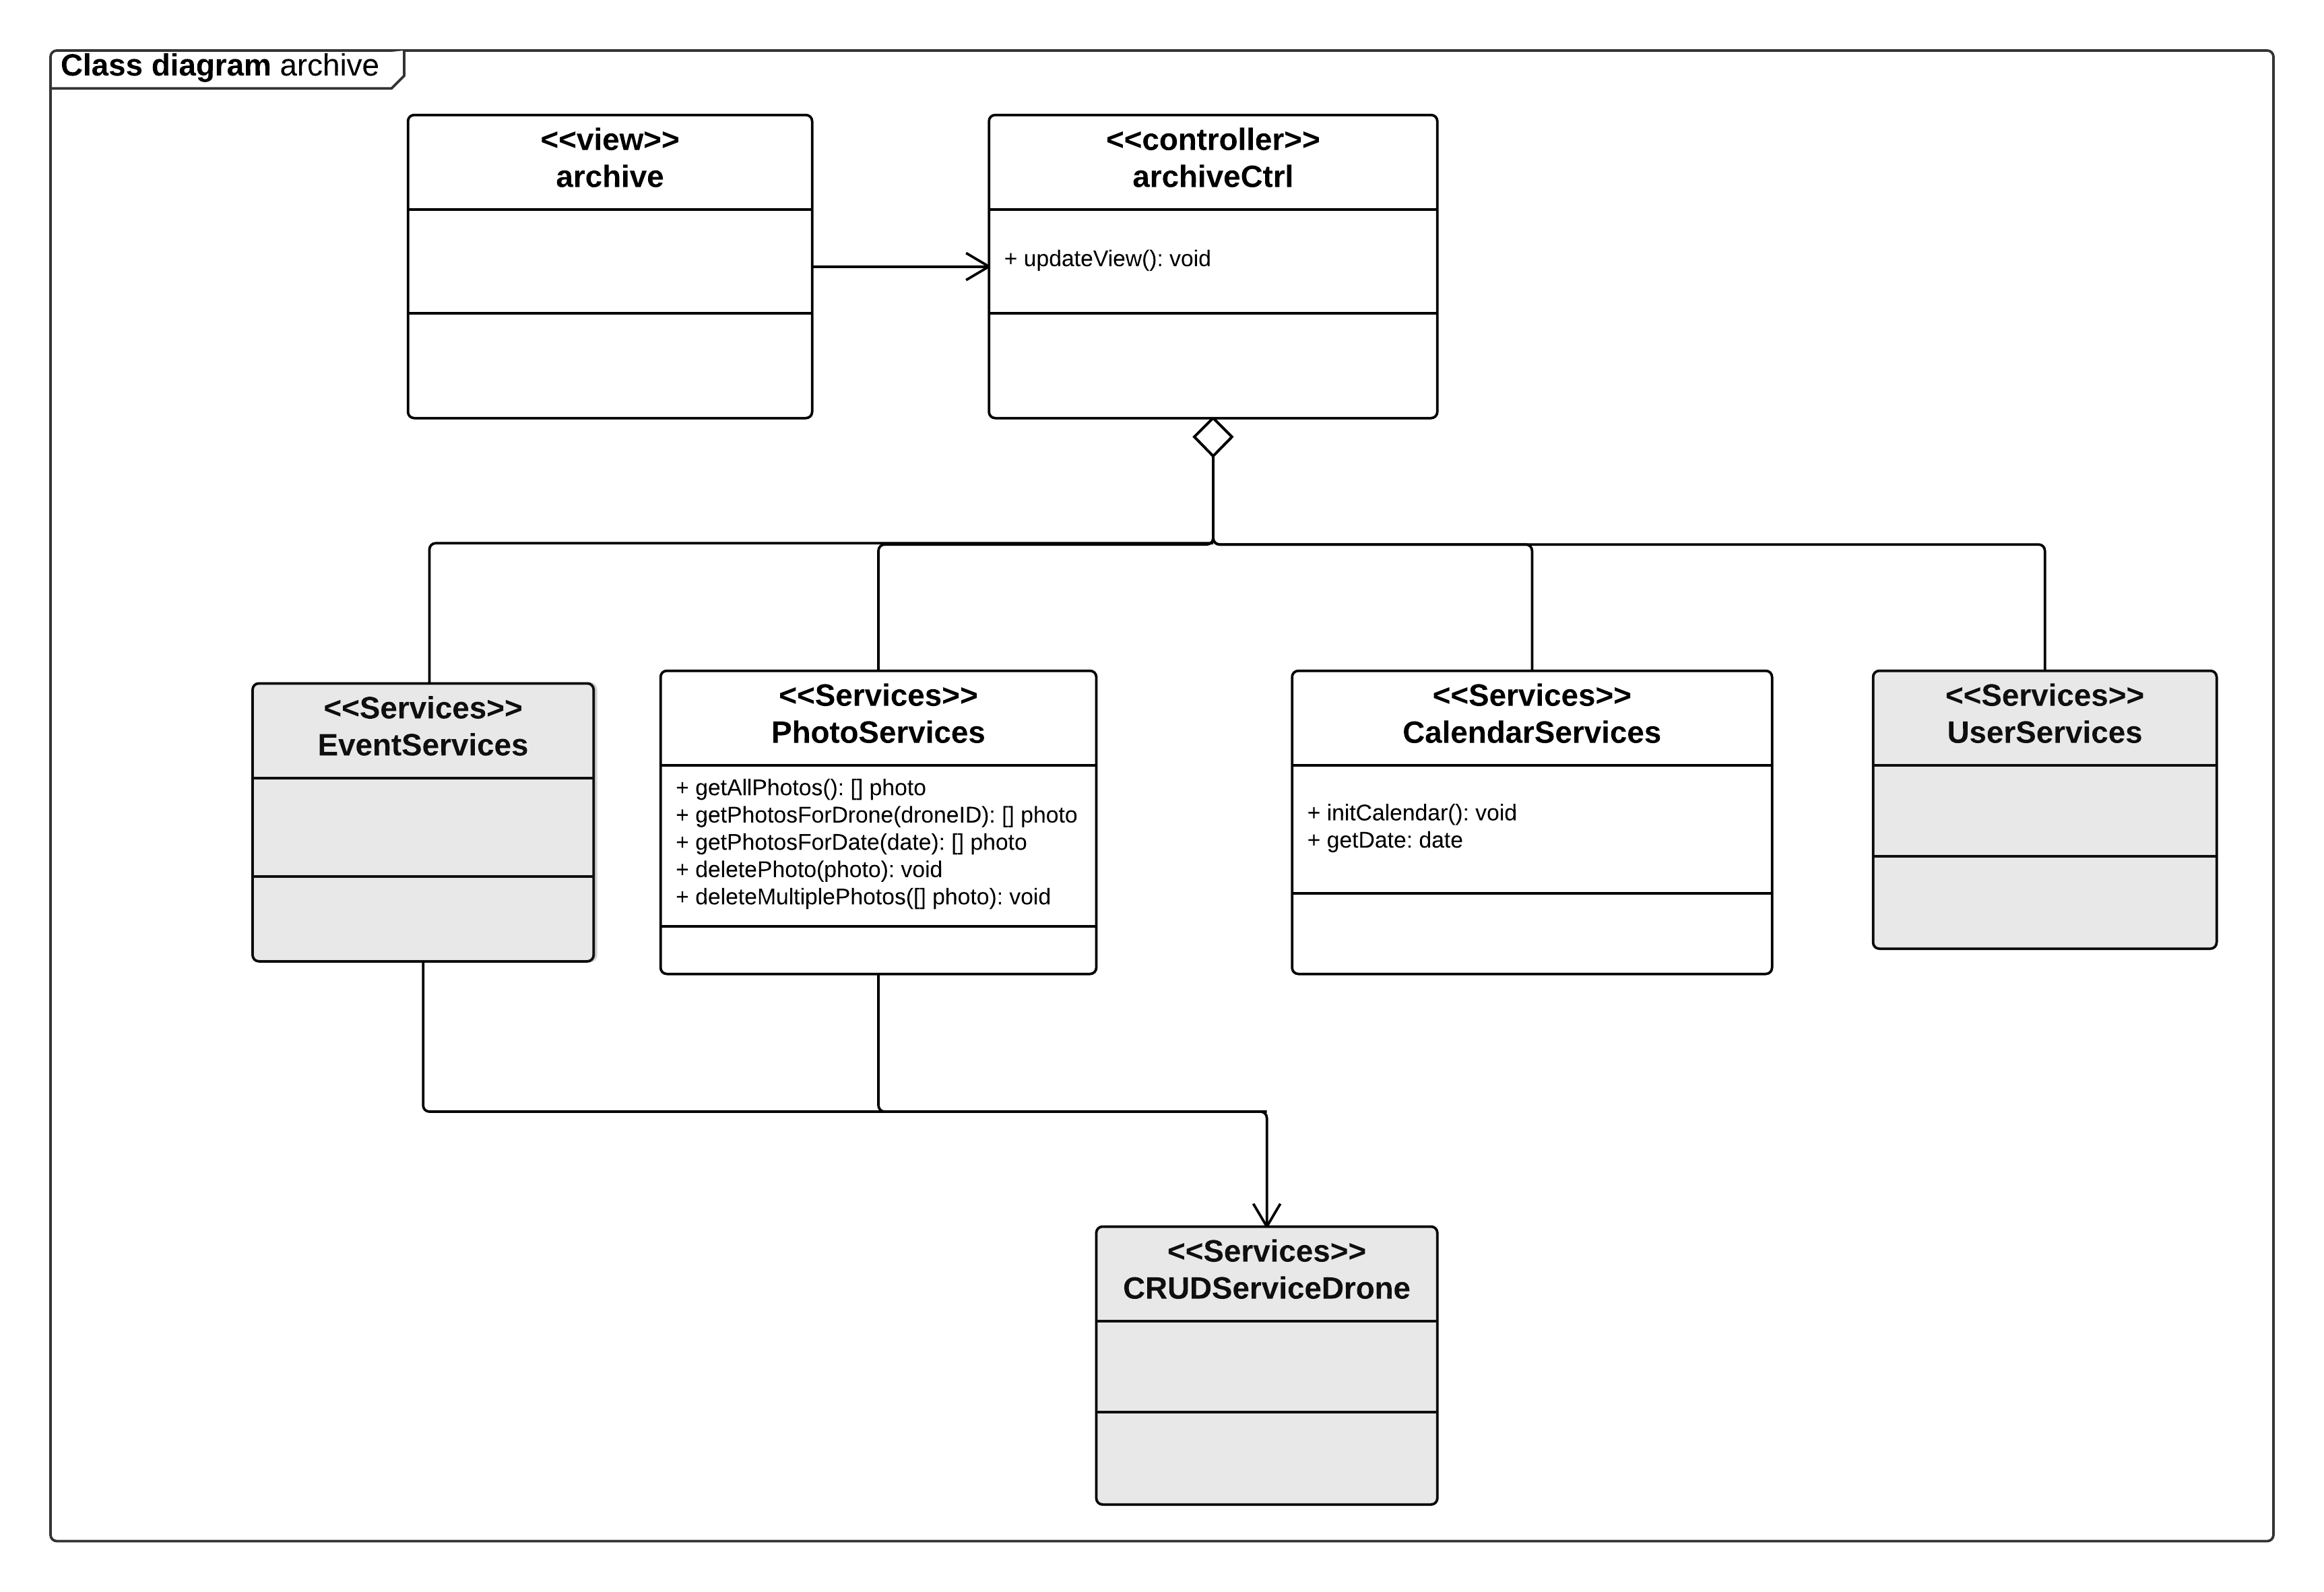
\includegraphics[width=1\textwidth]{Billeder/klasse_diagrammer/classdiagram_iteration3_server.png}
	\vspace{-0.5cm}
	\caption{Klassediagram \#iteration 3}
	\label{fig:classDiagram_iteration3}
\end{figure}

\textbf{archive}\\
Denne klasse er view'et tilhørende iteration tre. Denne klasse sammen med archiveCtrl skaber det endelig view som brugeren ser i sin browser når han besøger siden.

\textbf{archiveCtrl}\\
ArchiveCtrl klassen er controller klassen til iteration tre. Det er den eneste klasse der har direkte forbindelse til view'et, archiveCtrl klassen deler også hukommelse med view'et igennem two-way-binding med scopes.

\textbf{EventServices}\\
Denne klasse indeholder logikken om event håndtering. Klassen bruges til at hente en event liste, et enkelt event for en givet drone og sende et nyoprettet event til serveren via CRUDServiceDrone klassen.

\textbf{PhotoServices}\\
Denne klasse indeholder logikken om foto håndtering. Klassen bruges til at hente fotos via CRUDServiceDrone klassen, PhotoServices har også ansvaret for at slette uønskede billeder.

\textbf{CalendarServices}\\
Denne klasse indeholder logikken for kalenderen i view'et, klassen bruges til at oprette en kalender og navigering i kalenderen. Desuden bruges den også til at fortælle hvilke dato brugeren har valgt når han ønsker at finde billeder taget fra en givet dato.

\newpage

\textbf{UserServices}\\
Denne klasse blev oprettet i iteration et og bruges til at gemme information omkring hvilke bruger der er logget ind i systemet.

\textbf{CRUDServicesDrone}\\
Denne klasse fungere som bindeled imellem server og webapplikation. Klassen indeholder alt logikken omkring kommunikation til serveren, alle der vil kommunikere med serveren i systemet skal benytte sig af denne klasse. Igennem denne service er det muligt at hente, opdater og poste data til serveren.

\vspace{0.3cm}

\subsubsection*{State machine diagram}
\vspace{-0.3cm}
I state machine diagrammet på figur \ref{fig:Statemachine_iteration3}, vises de to states der eksisterer i iteration 3 og hvordan flowet imellem dem ser ud. Der eksisterer givet vis kun 2 states i iteration 3, men state machinen er medtaget fordi den fint illustrerer systemflowet.

\vspace{-0.2cm}
%kommentar
\begin{figure}[H]
	\centering
	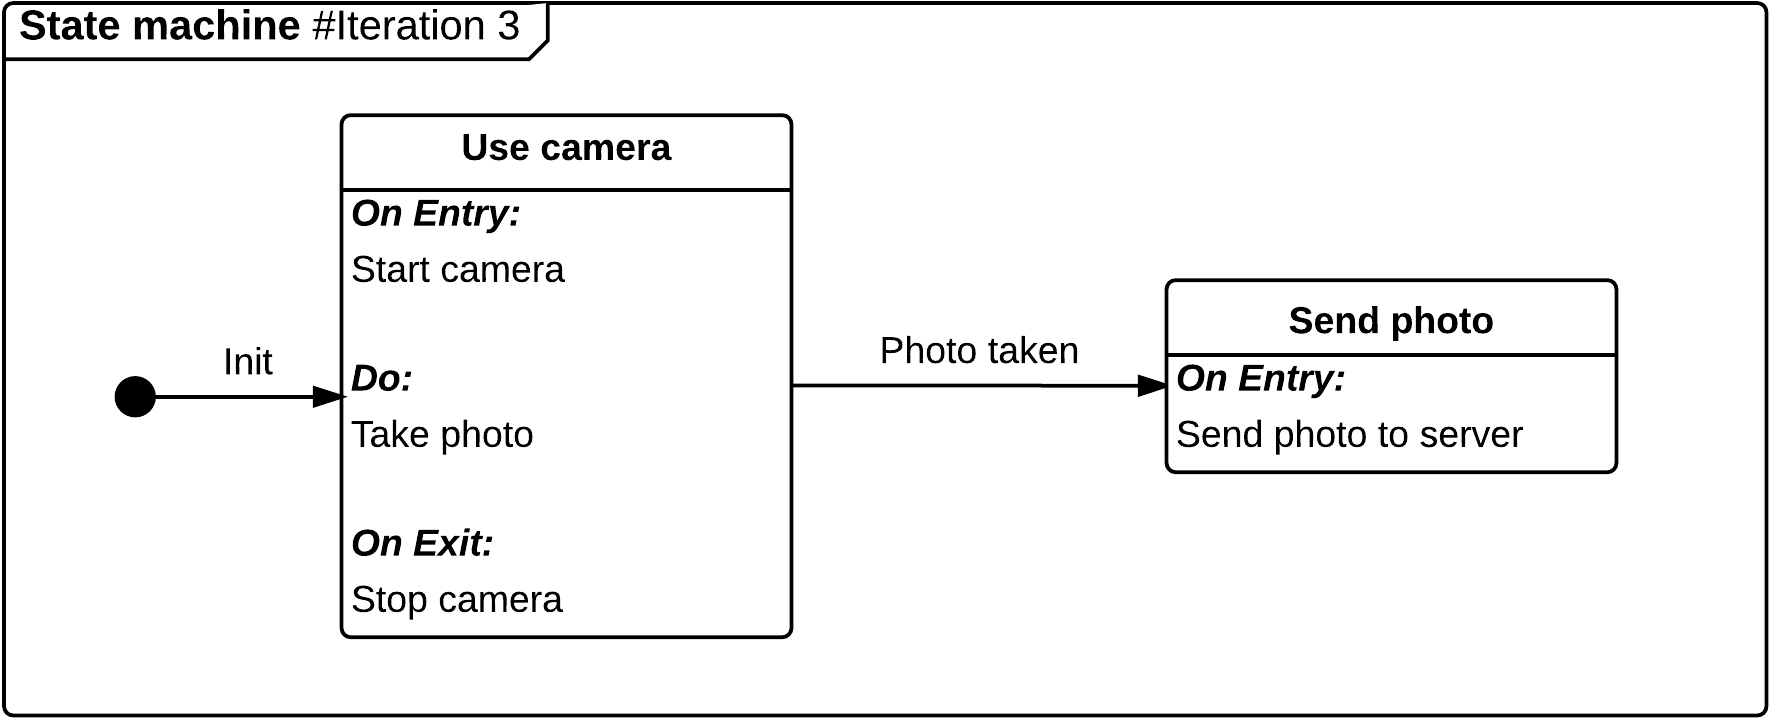
\includegraphics[width=0.9\textwidth]{Billeder/statemachine/State_iteration3.png}
	\caption{State machine \#iteration 3}
	\label{fig:Statemachine_iteration3}
\end{figure}



%\newpage
%\subsection{Iteration \#4}
I iteration 4 ønskes det at udvide systemet med anti kollision. Inden tilføjelsen af anti kollision kan dronen udelukkende flyve i områder uden forhindringer. Men med tilføjelsen af anti kollision vil det være muligt at flyve med dronen i normale områder med forskellige forhindringer. Hvordan systemet er tiltænkt at bruges beskrives i user story nedenfor:


\subsubsection*{User story}
Under flyvning kontrolleres det løbende hvorvidt der er et objekt foran dronen. Hvis der detekteres et objekt foran dronen, skal dronen holde om med at flyve fremad. I stedet skal dronen dreje horisontalt indtil der ikke længere er et objekt foran den. Når der er frit foran dronen fortsættes den afbrudte flyvning. 
Bruger af systemet har ingen direkte kontakt med anti kollisionssystemet. For bruger ses anti kollision blot som en ekstra feature, som gør dronen i stand til at flyve uden at kollidere med objekter foran sig.
 
%kommentar
\begin{figure}[H]
	\centering
	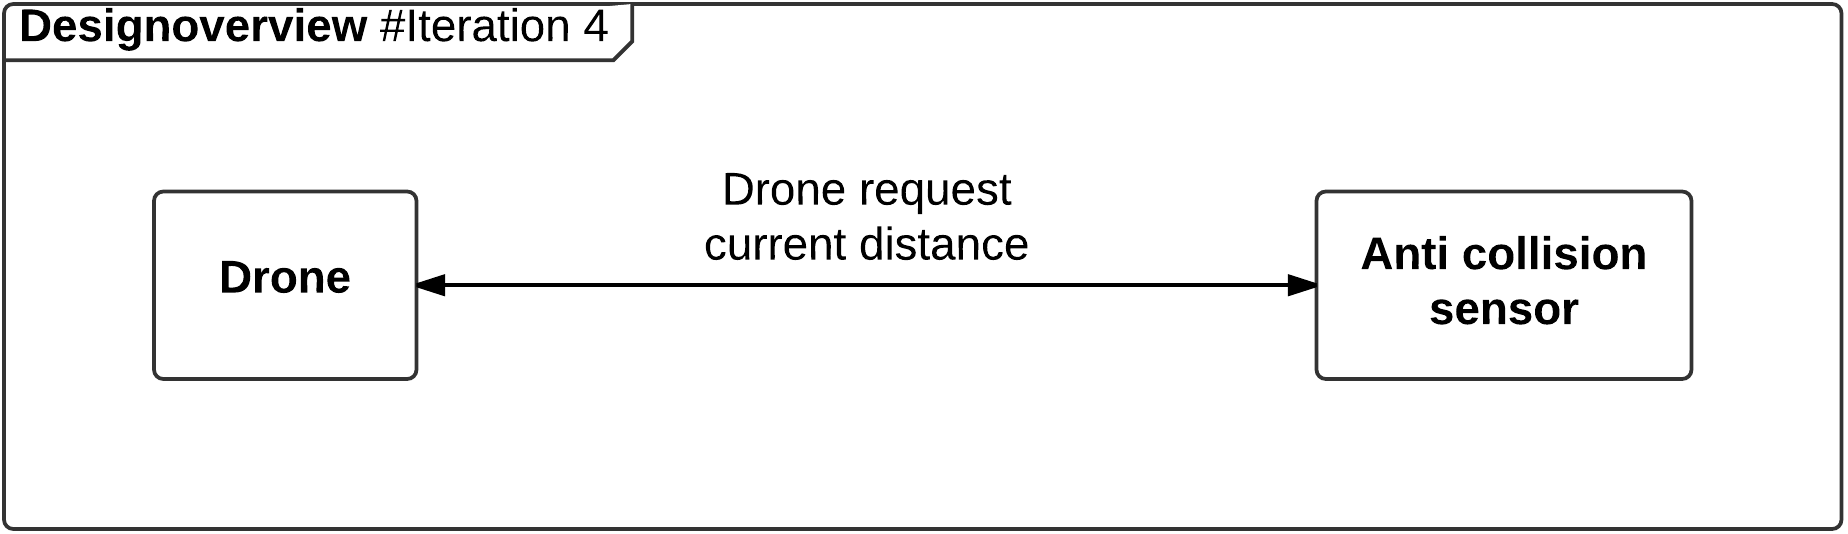
\includegraphics[width=1\textwidth]{Billeder/design_overview/design_overview_iteration4.png}
	\vspace{-.5cm}
	\caption{Designoverview \#iteration 4}
	\label{fig:design_overview_UC4}
\end{figure}


\newpage
\subsubsection*{Sekvens diagram}
\vspace{-0.2cm}
På sekvensdiagrammet vises de klasser der indgår og bruges i fjerde iteration. 
På diagrammet vises det hvordan afstanden til eventuelle objekter foran dronen kontrolleres. Hvis afstanden til et objekt er under den definerede kollisionsgrænse stoppes dronens fremdrift og der skiftes orientering. 


%kommentar
\begin{figure}[H]
	\centering
	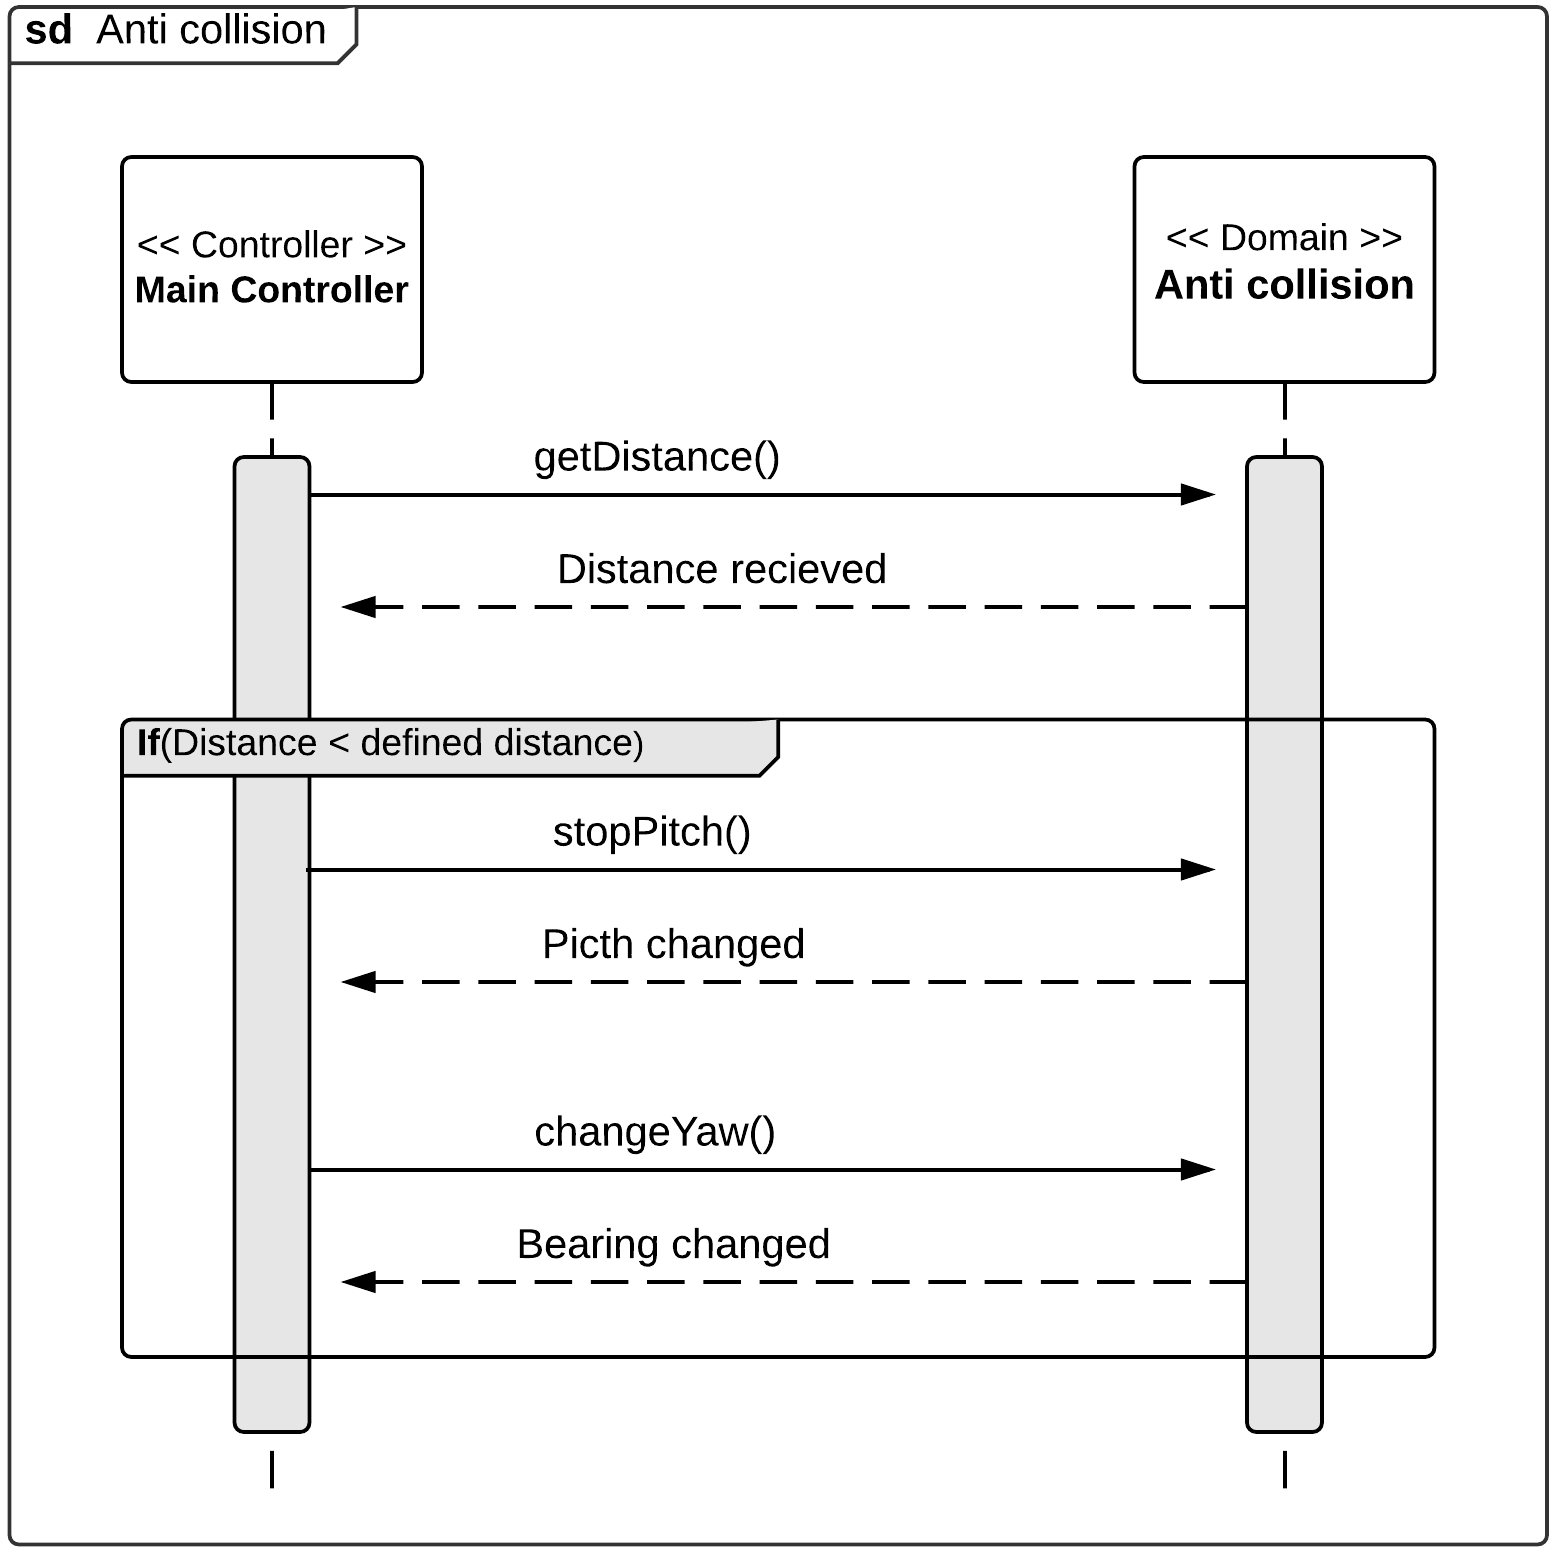
\includegraphics[width=0.8\textwidth]{Billeder/sekvens/sekvens_iteration4}
	\caption{Sekvens diagram \#iteration 4}
	\label{fig:Sekvens_diagram_iteration4}
\end{figure}



\subsubsection*{State machine diagram}
\vspace{-0.2cm}

I state machine diagrammet på figur \ref{fig:Statemachine_iteration4}, vises de to states der eksisterer i iteration 4. Desuden vises hvordan flowet imellem de to states ser ud.


%kommentar
\begin{figure}[H]
	\centering
	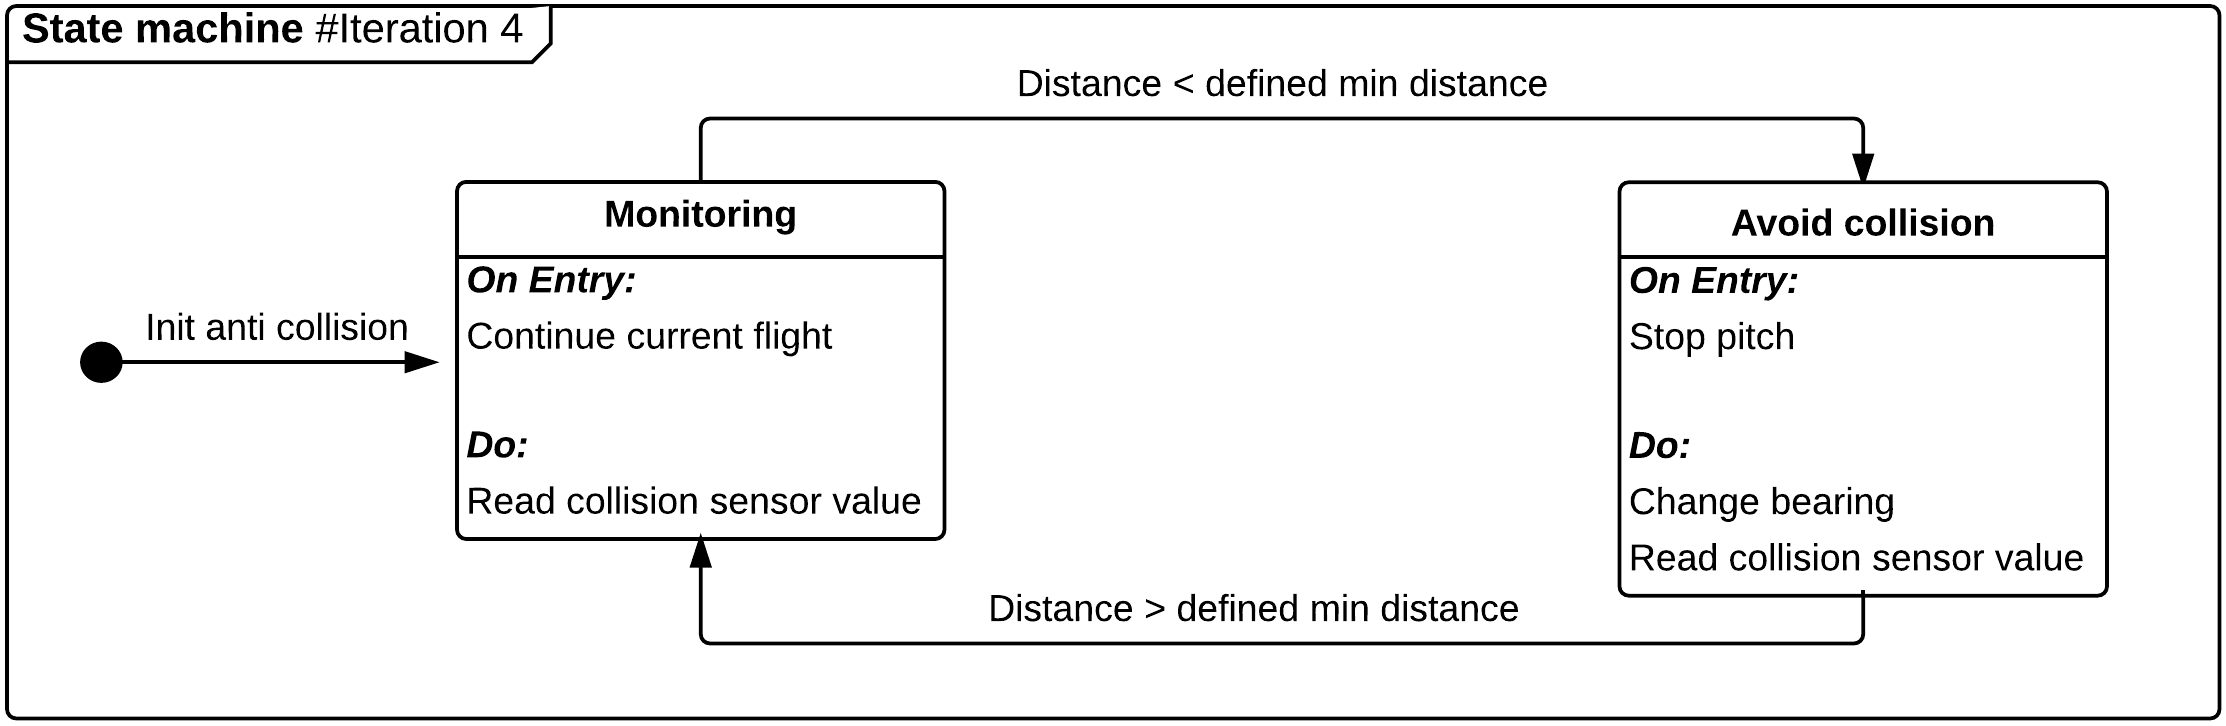
\includegraphics[width=1\textwidth]{Billeder/statemachine/State_iteration4.png}
	\vspace{-0.5cm}
	\caption{Statemachine \#iteration 4}
	\label{fig:Statemachine_iteration4}
\end{figure}



\subsubsection*{Klasse diagram}
\vspace{-0.1cm}

%kommentar
\begin{figure}[H]
	\centering
	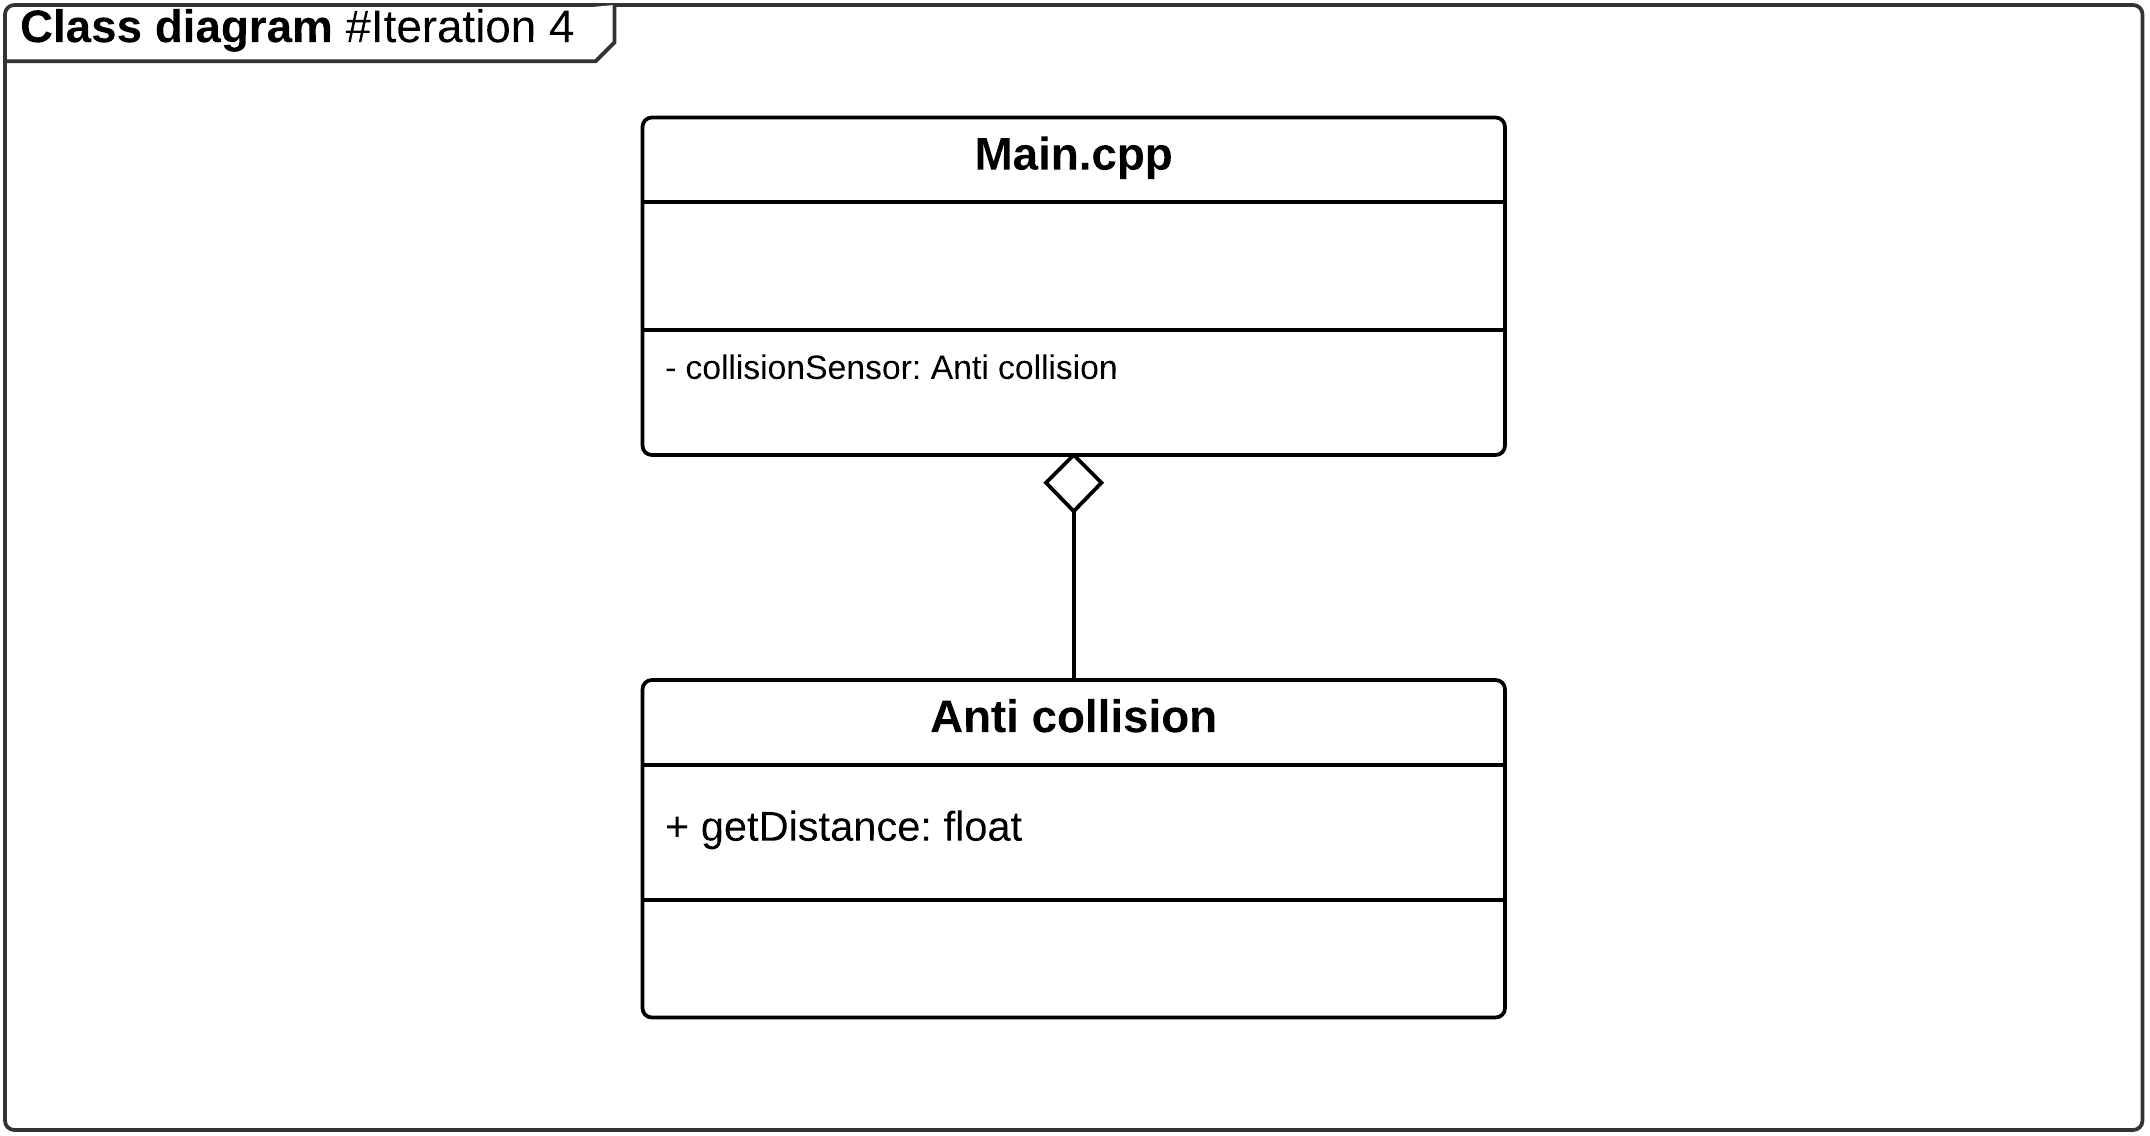
\includegraphics[width=1\textwidth]{Billeder/klasse_diagrammer/classdiagram_iteration4.png}
	\vspace{-0.5cm}
	\caption{Klasse diagram \#iteration 4}
	\label{fig:classDiagram_iteration4}
\end{figure}


\textbf{Main.cpp} \\
Main.cpp filen bruges til at sætte arduino board korrekt op, bla. sættes baudrate på de forskellige serielle forbindelser. Desuden bruges Main.cpp til at kalde og eksekverer forskellige klasse, objekter og funktioner.


\textbf{Anti collision} \\
Module\_3G er ansvarlig for alt kommunikation mellem drone og server. I klassen bruges to forskellige slags http request. Når der ønskes at trække information fra sever til drone gøres der brug af GET request mens der gøres brug af PUT request når dronen ønsker at informere server om ny lokation.



\newpage
\section{Process view}

Ingen af systemets centrale dele gør brug af tråde. Men systemet er opbygget således at afvikling af drone, website og server kan betragtes som 3 samtidige processer. Alle 3 dele bruges sideløbende i runtime og imellem dem flyder løbende data.

For systemets bruger ser det ud som om al information går direkte fra website til drone eller omvendt. Men reelt set er websitet og drone aldrig i direkte kontakt med hinanden. I stedet går al kommunikation til og fra serveren, som fungerer som et kommunikationslag. 

\vspace{-5pt}
\begin{figure}[H]
	\centering
	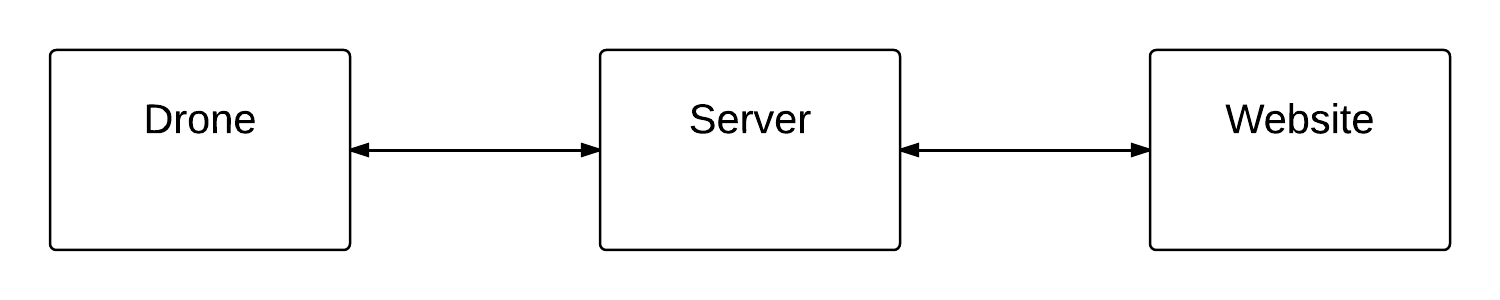
\includegraphics[width=0.7\textwidth]{Billeder/process_view}
	\vspace{0cm}
	\caption{Process view}
	\label{fig:process_view}
\end{figure}

\textbf{Server}\\
Serveren er passiv, hvilket betyder den aldrig tager initiativ til udveksling af data. Serveren foretager ingenting på egen hånd, den står i stedet og venter på at blive igangsat af drone eller website. 
 
\textbf{Drone} \\
I drone processen håndteres al styring af drone og kommunikation mellem drone og server. Når dronen er tændt og 3G/GPS modulet initialiseret, opdaterer dronen med få minutters interval egen GPS position for efterfølgende at sende serveren information om positionen. Desuden kontrollerer dronen løbende om der er en ny flyveopsætning tilgængelig på serveren. Hvis der er en ny flyveopsætning tilgængelig hentes den, og en ny flyvning påbegyndes. 

\textbf{Website}\\
Mellem server og website er der lavet en socket connection. Det betyder at indholdet af websitet opdateres hver gang der kommer nyt indhold på serveren. Desuden bruges websitet når systemets bruger ønsker at lave nye flyveopsætninger eller opdatere de nuværende.\\


Der er lagt megen energi i at designe og bygge systemet på en vis der tillader udvidelser og tilføjelser. Dels kan server nemt tilgås af flere forskellige websites og desuden kan websitet nemt håndtere flere droner og client’er samtidig.

\newpage
\subsection{Kommunikations timing}
For at de forskellige enheder i systemet kan kommunikere optimalt, er der blevet designet nogle bestemte kommunikations timing tabeller som skal overholders for at kunne kommunikere optimalt.\\
Disse tabeller skal køres i følgende rækkefølge:

\begin{enumerate}
	\item Dronen tændes
	\item Handlingen i tabel et udføres og gentages hvert 5min
	\item Handlingen i tabel to udføres og gentages hvert 5min
	\item Handlingen i tabel to retunere andet end 0
	\item Handlingen i tabel tre udføres
	\item Dronen er nu klar til at flyve
	\item Handlingen i tabel to gentages ikke mere
	\item Efter flyvning gentages det hele, bortset fra step 1
\end{enumerate}

\begin{table}[H]
	\centering
		\begin{tabular}{| m {1cm} | m {3cm} | m {4cm} | m {7cm} |}
			\hline
			Enhed & HTTP Request & Data & Handling \\ \hline
			Drone & PUT & Online og Location & Opdatere sin position og sætter sig online\\ \hline
			Server & Response & 200 OK & Giver ok svar tilbage \\ \hline
		\end{tabular}
	\caption{Kommunikation imellem drone og server step 1}
	\label{tab:kom_drone_server_1}
\end{table}

\begin{table}[H]
	\centering
		\begin{tabular}{| m {1cm} | m {3cm} | m {4cm} | m {7cm} |}
			\hline
			Enhed & HTTP Request & Data & Handling \\ \hline
			Drone & GET & NextEvent & Efterspørg nextevent værdig \\ \hline
			Server & Response & NextEvent & Retunere drone data, med nextevent \\ \hline
		\end{tabular}
	\caption{Kommunikation imellem drone og server step 2}
	\label{tab:kom_drone_server_2}
\end{table}

\begin{table}[H]
	\centering
		\begin{tabular}{| m {1cm} | m {3cm} | m {4cm} | m {7cm} |}
			\hline
			Enhed & HTTP Request & Data & Handling \\ \hline
			Drone & GET & Waypoint & Dronen henter waypoints tilhørende event\\ \hline
			Server & Response & Waypoints & Retunere waypoints tilhørende event \\ \hline
			Drone & PUT & NextEvent = 0 & Dronen ændre sin NextEvent værdig til 0 \\ \hline
			Server & Response & 200 OK & Giver ok svar tilbage \\ \hline
		\end{tabular}
	\caption{Kommunikation imellem drone og server step 3}
	\label{tab:kom_drone_server_3}
\end{table}

\newpage
\section{Data view}

\subsection{Database design}

\subsubsection*{Mission}
Databasen har til formål at vise systemets brugere hvilke droner de har til rådighed. Blandt andet skal det være muligt for bruger at se hvilke droner der er ude og flyve og hvilke der ikke er aktive. Databasen tracker også hvilke events der foregår med hver drone og danner historik over det. Eksempler på events kan være information om flyveruten og om der tages billeder på flyveturen.

\subsubsection*{Design}
På figur \ref{fig:database_design} ses det overordnede designet af databasen. Som beskrevet i foranalysen er det valgt at gøre brug af en SQLight database. Alt kommunikation til og fra databasen vil fungere igennem et database API. Database API'et er et REST API som er udviklet ved brug af Django og Django REST frameworket. Ved kombination af disse Django og Django REST fås en databasen som er "indkapslet" og kun kan tilgås gennem API'et. Kommunikationen til og fra API'et foregår ved sende eller modtage JSON filer til API'ets endpoints. Hjælpe tabellerne som ses på figur \ref{fig:database_design} bliver automatisk oprettet af django frameworket, hvilket betyder de senere ikke er til at finde i koden for databasen. Hjælpe tabellerne er dog tegnet med på diagrammet, da de eksistere i systemet og fordi de kan være med til at forstærke forståelsen af databasen. 

\vspace{-5pt}
\begin{figure}[H]
	\centering
	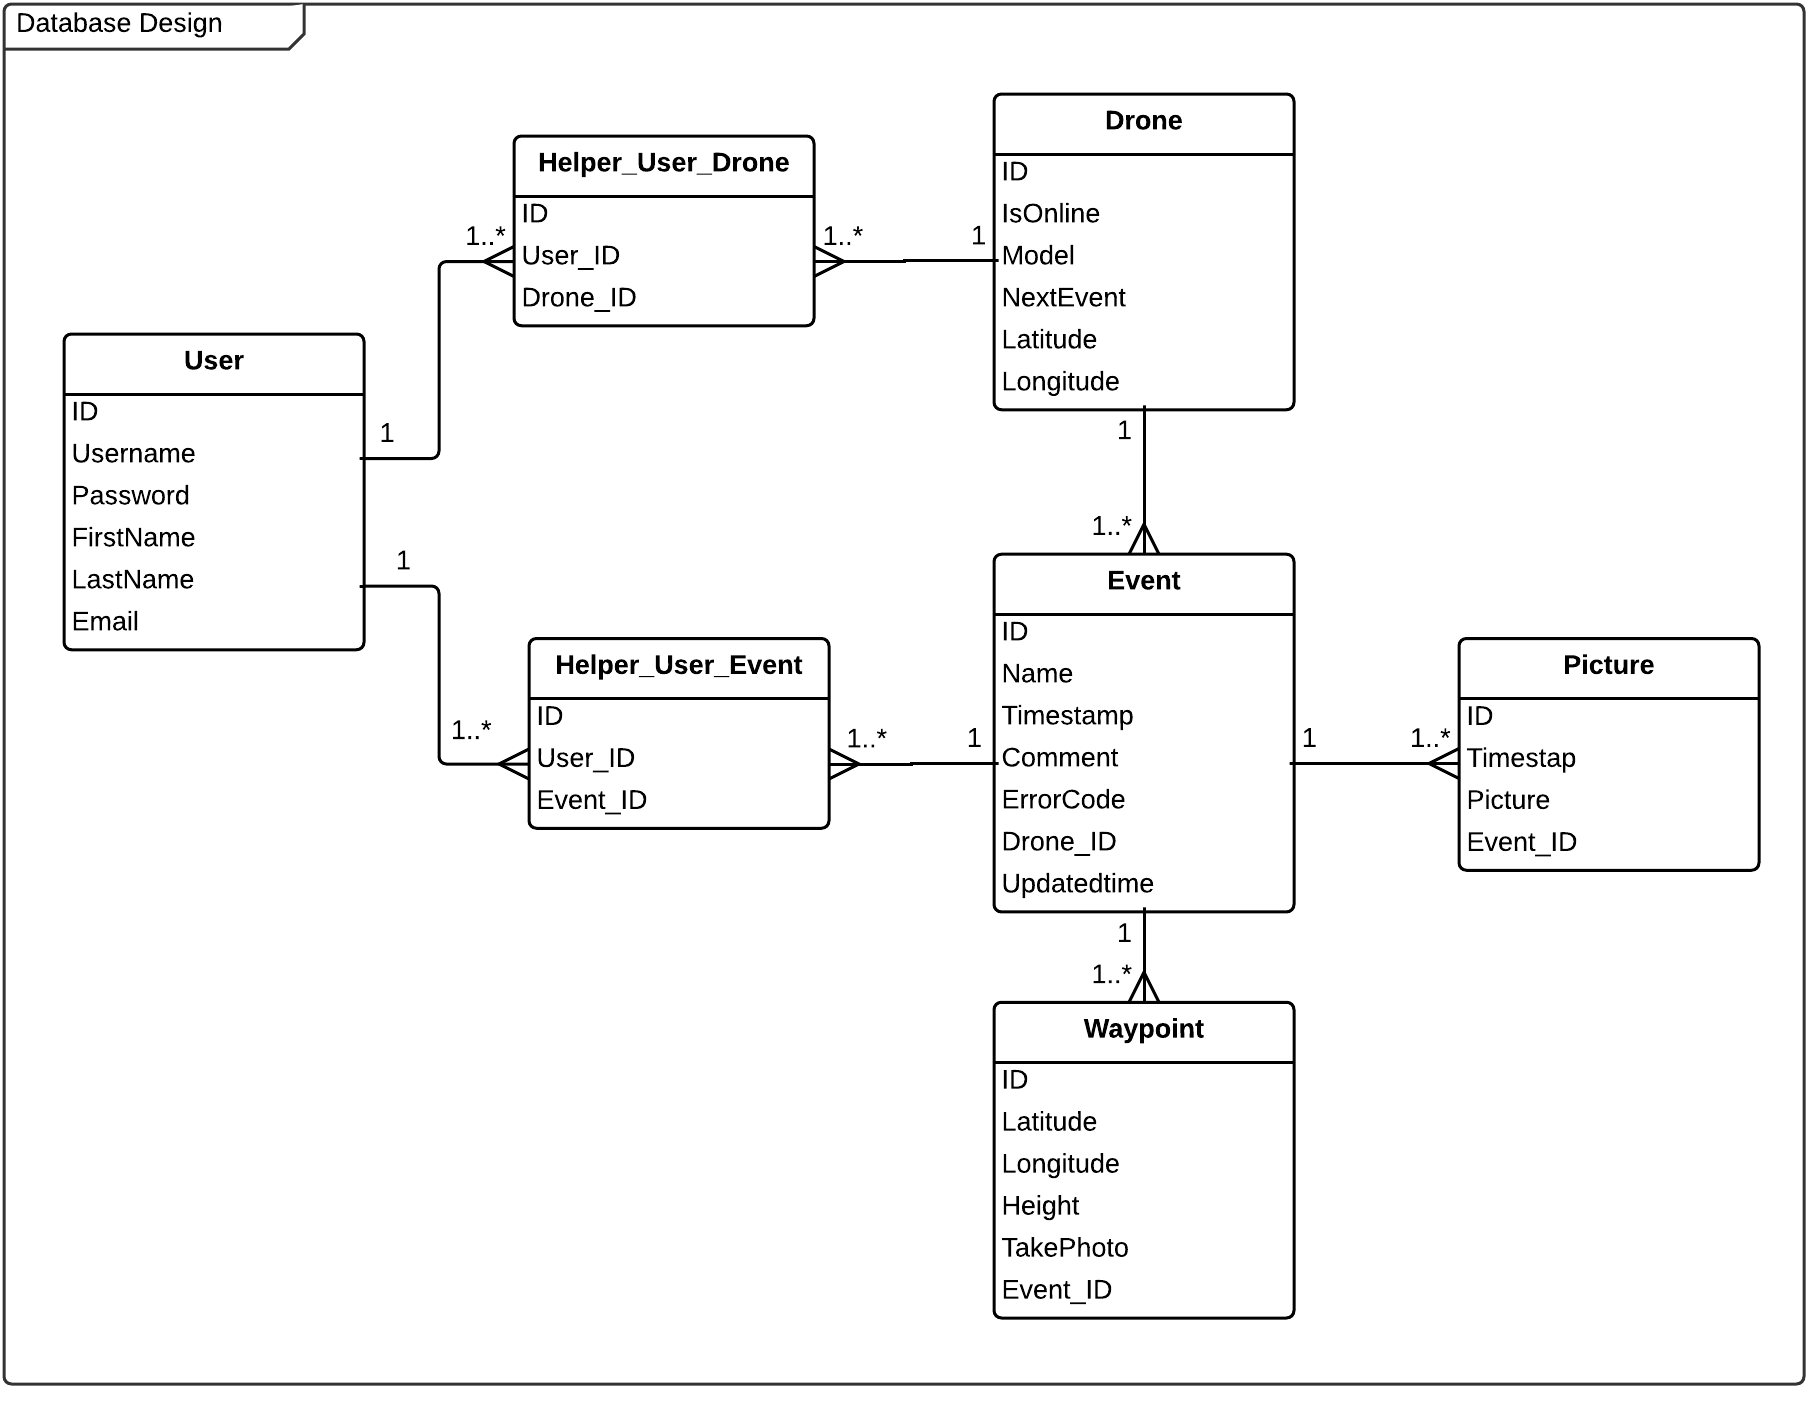
\includegraphics[width=1\textwidth]{Billeder/database/database_design.png}
	\vspace{-.5cm}
	\caption{Database design}
	\label{fig:database_design}
\end{figure}

\subsubsection*{Tilgængelige endpoints}
De tilgængelige endpoint i API'et er følgende:

\begin{table}[H]
\begin{tabular}{| p{3cm}| p{11.5cm}|}
\hline
Endpoint:	 							& \textbf{\textit{api/waypoints/}}\\\hline
Allows:									& POST, OPTIONS, GET\\\hline
Content-Type:						& application/json\\\hline 
Indehold:								& Giver adgang til waypoints tabellen, med muglighed for at tilføje nye waypoints\\\hline 
Kommentar:							& Det er muligt at tilføje "?format=json" til URL'en for at få dataen i ren json format\\\hline
\end{tabular}
\caption{Waypoint endpoint}
\label{waypoint_endpoint}
\end{table}

\begin{table}[H]
\begin{tabular}{| p{3cm}| p{11.5cm}|}
\hline
Endpoint:	 							& \textbf{\textit{api/users/}} \\\hline
Allows:									& OPTIONS, GET\\\hline
Content-Type:						& application/json\\\hline 
Indehold:								& Giver adgang til user tabellen\\\hline 
Kommentar:							& Det er muligt at tilføje "?format=json" til URL'en for at få dataen i ren json format\\\hline
\end{tabular}
\caption{User endpoint}
\label{user_endpoint}
\end{table}

\begin{table}[H]
\begin{tabular}{| p{3cm}| p{11.5cm}|}
\hline
Endpoint:	 							&\textbf{\textit{api/pictures/}} \\\hline
Allows:									& POST, OPTIONS, GET\\\hline
Content-Type:						& application/json\\\hline 
Indehold:								& Giver adgang til pictures tabellen, med mulighed for at tilføje nye billeder\\\hline 
Kommentar:							& Det er muligt at tilføje "?format=json" til URL'en for at få dataen i ren json format\\\hline
\end{tabular}
\caption{Picture endpoint}
\label{picture_endpoint}
\end{table}

\begin{table}[H]
\begin{tabular}{| p{3cm}| p{11.5cm}|}
\hline
Endpoint:	 							&\textbf{\textit{api/events/}}\\\hline
Allows:									& POST, PUT, OPTIONS, GET\\\hline
Content-Type:						& application/json\\\hline 
Indehold:								& Giver adgang til event tabellen, med mulighed for at oprette nye events og opdatere dem\\\hline 
Kommentar:							& Det er muligt at tilføje "?format=json" til URL'en for at få dataen i ren json format\\\hline
\end{tabular}
\caption{Event endpoint}
\label{event_endpoint}
\end{table}

\begin{table}[H]
\begin{tabular}{| p{3cm}| p{11.5cm}|}
\hline
Endpoint:	 							&\textbf{\textit{api/drones/}}\\\hline
Allows:									& POST, OPTIONS, GET\\\hline
Content-Type:						& application/json\\\hline 
Indehold:								& Giver adgang til drone tabellen, med mulighed for at tilføje nye droner\\\hline 
Kommentar:							& Det er muligt at tilføje "?format=json" til URL'en for at få dataen i ren json format\\\hline
\end{tabular}
\caption{Drones endpoint}
\label{drones_endpoint}
\end{table}

\begin{table}[H]
\begin{tabular}{| p{3cm}| p{11.5cm}|}
\hline
Endpoint:	 							&\textbf{\textit{api/drones/\#/}}\\\hline
Allows:									& PUT, OPTIONS, GET\\\hline
Content-Type:						& application/json\\\hline 
Indehold:								& Giver adgang til en record i drone tabellen, med mulighed for at opdatere droner\\\hline 
Kommentar:							& Det er muligt at tilføje "?format=json" til URL'en for at få dataen i ren json format\\\hline
\end{tabular}
\caption{Single drone endpoint}
\label{single_drone_endpoint}
\end{table}

\newpage
\subsection{Detaljeret database beskrivelse}

\subsubsection*{User table}
Tabellen indeholder data om systemets brugere. Tabellen gør det via Foring keys muligt for systemets brugere at tilgå droner, events og de gemte flyruter i systemet.
\vspace{-5pt}
\begin{figure}[H]
	\centering
	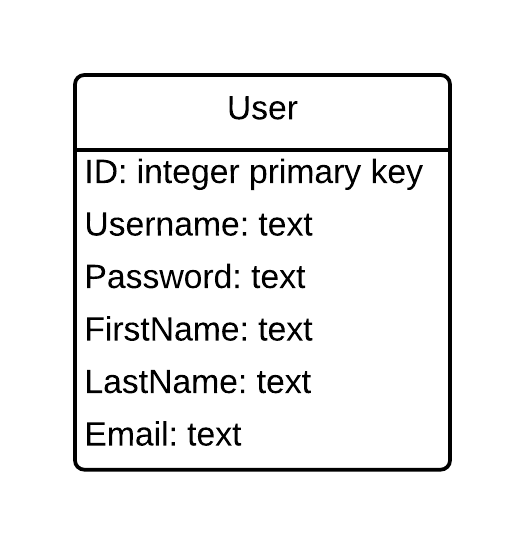
\includegraphics[width=0.5\textwidth]{Billeder/database/UserTabel.png}
	\vspace{-5pt}
	\caption{User table}
	\label{fig:user_table}
\end{figure}

\begin{table}[H]
\begin{tabular}{| p{3cm}| p{11.5cm}|}
\hline

Formål	 							& At holde data om brugere i systemet, samt tjekke om brugere eksisterer, når de forsøger at logge på webapplikation.\\\hline
Forbindelser						& Tabellen har en foreing key til at hjælpe tabellerne: Helper User Drone og Helper User Event.\\\hline
Attributter						& \begin{itemize}
												\item ID: Primary key.
												\item Username: Brugernavnet til systemet. Max length: 50 char
												\item Password: Brugerens kode. Max length: 50 char
												\item FirstName: Brugers fornavn. Max length: 50 char
												\item LastName: Brugerens efternavn. Max length: 50 char
												\item Email: Brugerens email adresse.
											\end{itemize} \\\hline 
\end{tabular}
\caption{User table}
\label{tab:user_table}
\end{table}
\newpage
\subsubsection{Event table}
Tabellen indeholder data om events i systemet. Tabellen fungere som omdrejnings punkt i databasen. Droner kan tilkobles et event, billeder bliver tilføjet til et event og waypoints bliver tilføjet til et event.
\vspace{-5pt}
\begin{figure}[H]
	\centering
	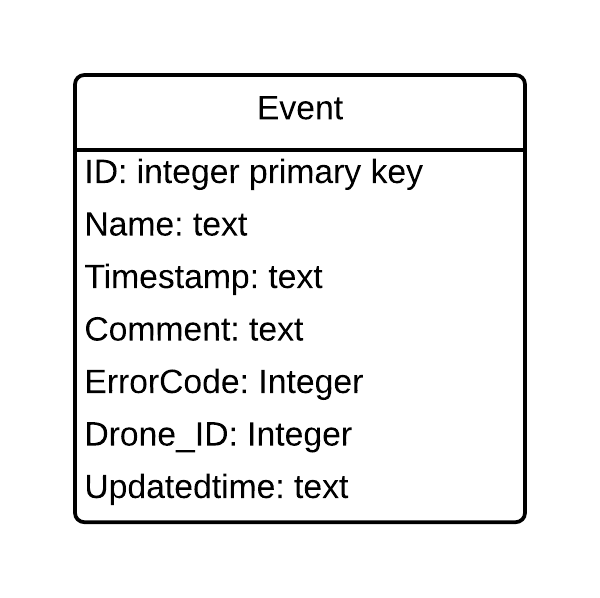
\includegraphics[width=0.5\textwidth]{Billeder/database/EventTable.png}
	\vspace{-5pt}
	\caption{Event table}
	\label{fig:event_table}
\end{figure}

\begin{table}[H]
\begin{tabular}{| p{3cm}| p{11.5cm}|}
\hline

Formål	 							& Holde data om events i systemet.\\\hline
Forbindelser						& Tabellen har en foreing key til user tabellen med en mange til mange relation. Drone-, waypoint- og picture-tabellen har foreing keys til tabellen.\\\hline
Attributter						& \begin{itemize}
												\item ID: Primary key.
												\item Name: Navnet på det givet event. Max length: 100 char
												\item Timestamp: Timestamp for oprettelse: Datefield
												\item Updated: Timestamp for opdaterede: Datefield
												\item Comment: Kommentar til givet event. Max length: 100 char
												\item ErrorCode: Fejlkode hvis fejl opstår under flyvning: Integer
												\item UserId: Mange til mange relation til user tabellen: Foreingkey
											\end{itemize} \\\hline 
\end{tabular}
\caption{Event table}
\label{tab:event_table}
\end{table}
\newpage
\subsubsection{Picture table}
Tabellen indeholder data om billeder taget af dronen i systemet, samt selve billederne. Billeder bliver gemt i en blob type, som bare er binær-data i databasen.
\vspace{-5pt}
\begin{figure}[H]
	\centering
	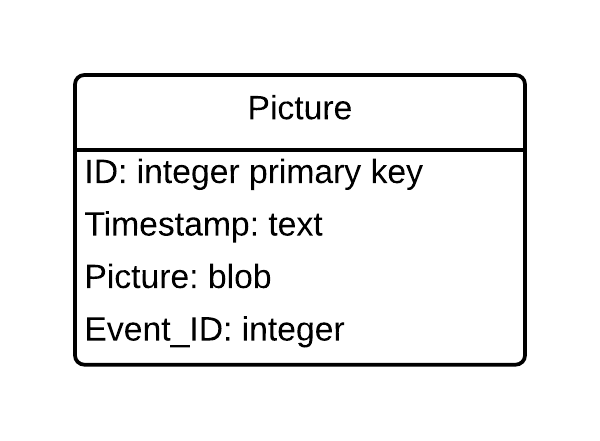
\includegraphics[width=0.5\textwidth]{Billeder/database/PictureTable.png}
	\vspace{-5pt}
	\caption{Picture table}
	\label{fig:picture_table}
\end{figure}

\begin{table}[H]
\begin{tabular}{| p{3cm}| p{11.5cm}|}
\hline

Formål	 							& Holde data om billeder i systemet og selve billederne.\\\hline
Forbindelser						& Tabellen har en foreing key til event tabllen.\\\hline
Attributter						& \begin{itemize}
												\item ID: Primary key.
												\item Name: Navnet på det givet event. Max length: 100 char
												\item Timestamp: Timestamp for oprettelse: Datefield
												\item Picture: blob: Udefinerbar størrelse binær data
												\item Event ID: Relation til event tabellen: Foreingkey
											\end{itemize} \\\hline 
\end{tabular}
\caption{Picture table}
\label{tab:picture_table}
\end{table}
\newpage
\subsubsection*{Waypoint table}
Tabellen indeholder alle waypoints som brugeren har oprettet i systemet. Hvert waypoint i tabellen indeholder information om gps-koordinatet, højden og om der skal tages et billede ved lokationen eller ej.
\vspace{-5pt}
\begin{figure}[H]
	\centering
	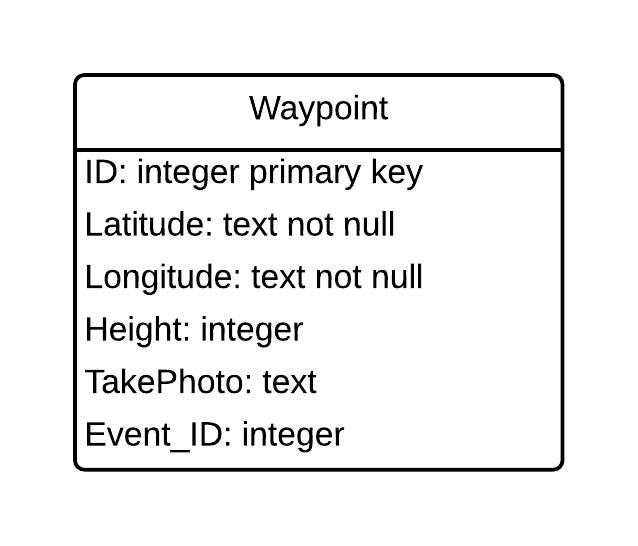
\includegraphics[width=0.5\textwidth]{Billeder/database/WaypointTable.png}
	\vspace{-5pt}
	\caption{Waypoint table}
	\label{fig:waypoint_table}
\end{figure}

\begin{table}[H]
\begin{tabular}{| p{3cm}| p{11.5cm}|}
\hline

Formål	 							& Holde data om waypoints i systemet.\\\hline
Forbindelser						& Waypoint tabellen har en foreing key til event tabellen.\\\hline
Attributter						& \begin{itemize}
												\item ID: Primary key.
												\item Latitude: Requried text felt. Max length: 100 char
												\item Longitude: Requried text felt. Max length: 100 char
												\item Height: Integer
												\item Event ID: Relation til event tabellen: Foreing key
											\end{itemize} \\\hline 
\end{tabular}
\caption{Waypoint table}
\label{tab:waypoint_table}
\end{table}
\newpage
\subsubsection*{Drone table}
Tabellen indeholder alle droner som er oprettet i systemet. Bruger har mulighed for at tilføje flere droner.
\vspace{-5pt}
\begin{figure}[H]
	\centering
	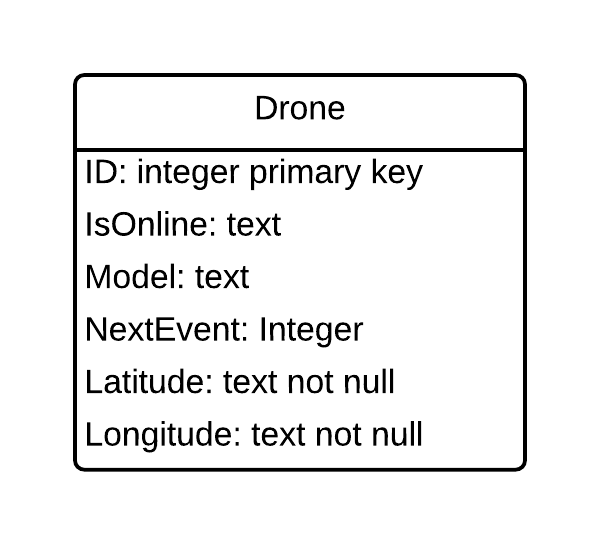
\includegraphics[width=0.5\textwidth]{Billeder/database/DroneTable.png}
	\vspace{-5pt}
	\caption{Drone table}
	\label{fig:drone_table}
\end{figure}

\begin{table}[H]
\begin{tabular}{| p{3cm}| p{11.5cm}|}
\hline

Formål	 							& Holde information om hver drone i systemet.\\\hline
Forbindelser						& Drone tabellen har en foreing key til event tabellen.\\\hline
Attributter						& \begin{itemize}
												\item ID: Primary key.
												\item IsOnline: Status for dronen: Boolean værdig
												\item Model: Modeltype: Text field: Max length 50 char
												\item NextEvent: Events for dronen: Integer field
												\item Latitude: Dronens GPS lokation: Max length 100 char  
												\item Longitude: Dronens GPS lokation: Max length 100 char
											\end{itemize} \\\hline 
\end{tabular}
\caption{Drone table}
\label{tab:drone_table}
\end{table}



\newpage
\section{Deployment view}

\subsection{HTTP 1.1 protokol}

For at kunne udveklse informationer mellem server og drone er der blevet anvendt en protokol. Protokollen er blevet valgt på baggrund af kommunikations måden, men også ifht. kommunikationen mellem websitet og serveren. Websitet kommer til at kommunikere med serveren på samme måde som dronen vil, derfor er det passende at bruge samme protokol. 
Valget blev at anvende HTTP protokollen. HTTP er en protokol der befinder sig i applikations laget, som er det øverste lag i internet protokollen. Det er dette lag der håndterer kommunikationen eller udveksling af data over internettet. 
Clienten (I dette tilfælde dronen) laver et request til serverens URL ved at oprette en TCP forbindelse. Når denne forbindelse er oprettet, kan clienten kalde http requesten i form af forskellige kommandoer. De forskellige kommandoer kan beskrives som CRUD (Create, Read, Update \& Delete) metoder. 
Med disse kommandoer vil dronen være i stand til at kommunikere og få de information der er nødvendige for at kunne flyve til de forskellige koordinater.

Dronen anvender HTTP 1.1, da der er flere metoder at gøre brug af. 
Dronen bruger 3 metoder til at kommunikere med serveren: GET, POST \& PUT. 
\begin{itemize}
	\item GET: henter data fra serveren.
	\item POST: Sender data til serveren, hvor serveren så opretter objektet.
	\item PUT: Opdaterer data på serveren og hvis der ikke allerede findes den type data, opretter serveren objektet.
\end{itemize}

Når clienten laver en get request, vil serveren svare med en header og body. Headeren vil indeholde en status besked. Denne status besked fortæller om requesten er gået igennem eller om der er sket en fejl undervejs.Ved en succesfuld modtagelse, vil der stå http 200 OK. Udover status beskeden vil header også bestå af meta data, som fx. hvilket format beskeden er i. 
Bodyen der modtages indeholder således de ønskede data fra serveren.

Ved et post eller put request, skal dronen sende en header fil samt en body med de data der ønskes udvekslet til serveren. 
Ved put er det vigtigt at det data der ønskes sendt har samme format som det der ligger på serveren, ellers melder status beskeden at der er en fejl. 




% http://en.wikipedia.org/wiki/Hypertext_Transfer_Protocol


\newpage
\section{Implementation view}

INDLEDENDE BESKRIVELSE MANGLER!

\subsection{Opsætning af udviklings IDE til Arduino}

- Setup guide
- 


For at kunne anvende Atmel til projektet, skulle det først sættes op med de rigtige stier, clock indstillinger mm. Her blev der fulgt en guide \footnote{http://www.engblaze.com/tutorial-using-atmel-studio-6-with-arduino-projects/}, som trin for trin beskriver opsætningen af Atmel IDE'et. Guiden blev kun fulgt til og med \textit{"Build your project”}. 
For at kunne anvende Arduino biblioteker i Atmel kræver det at Arduino 1.0 eller højere er installeret. Det er muligt at tilføje eksterne biblioteker, ved at vælge Project i menuen og derefter vælge: "Add Existing Item", dette tilføjer et bibliotek til ens bibliotek. Derudover skal eksterne biblioteker også tilføjes compiler stien. Dette gøres ved at vælge Projects -> projektnavn properties. Her inde skal man vælge menuen ToolChain og ved Configurations vælge: All Configurations. Under menuen GNU C++ compiler vælges Directories, her inde skal man skrive stien for de eksterne biblioteker.

Megunolink er et program med en brugergrænseflade der kan anvendes til at sende og modtage seriel data fra en arduino.
For at kunne bruge megunolink sammen med Arduino kræver det at det bliver sat op på den rigtige måde.
Først hentes en gratis udgave af MegunoLink: MegunoLink Lite \footnote{http://www.megunolink.com/megunolink-lite/megunolink-lite-plotting-tool/}.

Efter installationen skal megunolink sættes op til at kunne compilere til en arduino.

\begin{enumerate}
	\item I configuration benyttes "use custom path" og ved AVRDude stien linkes til stien med AVRDude til arduino og configurationens stien. 
	\item I dropdown menuen vælges den arduino der skal bruges til projektet.
\end{enumerate}

\newpage

\begin{figure}[H]
	\centering
	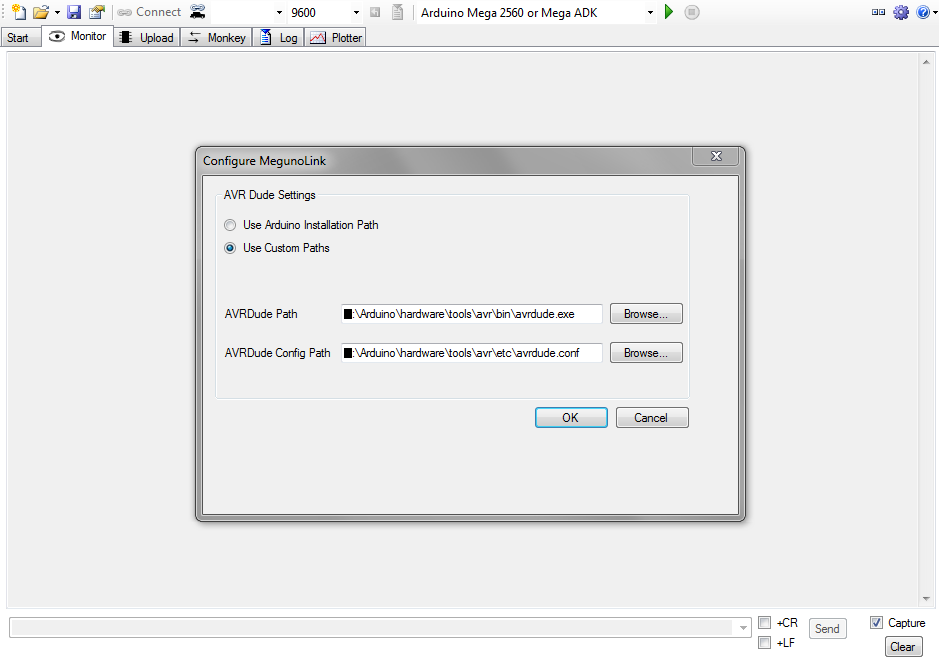
\includegraphics[width=0.85\textwidth]{Billeder/implementation/megunolink_config.png}
	\vspace{-.5cm}
	\caption{MegunoLink config}
	\label{fig:meglinkconf}
\end{figure}

For at kunne compilere, skal der linkes til projektets source fil. Hvis dette er udført korrekt, burde det være muligt at uploade source filen til arduino.

\subsection{Opsætning af eksterne bibliotekter til Atmel}

Når dronen henter informationer ned fra serveren, sker det med en karakter af gangen. Dette giver nogle vanskeligheder ifht. at skulle sortere i dataet der er modtaget. Når der hentes data, kan det bl.a. være længde- og breddegrader. Når det modtages, ved man ikke hvilken plads det ligger på i arrayet og hvilken størrelse værdierne har. Man kan, mellem server og drone, forud definere størrelserne der sendes/modtages, men det er hverken dynamisk eller præcis. Fra server siden er flyveopsætningen defineret som JSon objekter, hvilket er overskueligt og nem at sortere i. \\
I Atmel eller arduino findes der ikke et standard JSon bibliotek, der kan søge eller erstatte informationerne i et JSon objekt. Derfor har det været nødvendigt at finde et bibliotek der har kunnet tage denne type fil og bearbejde det som almindeligt data. Det anvendte bibliotek hedder aJson\footnote{https://github.com/interactive-matter/aJson} og er et frit tilgængeligt JSon bibliotek.Dette bibliotek er kombatibel med arduino. Ved hjælp af dette bibliotek, er det blevet muligt at hente flyveopsætningen fra serveren og afkode, oprette og ændre i dataet.

\newpage
\subsection{Opsætning af server}
Dette afsnit har til formål at beskrive hvordan et udviklingsmiljø sættes op på en givet maskine, så vider udvikling af systemet kan finde sted. Afsnittet forklarer også hvilke tredjeparts teknologier der er anvendt og eventuelle afhængigheder.

\subsubsection*{OS}
Det anbefales at udviklingen finder sted på en OS X eller Linux maskine, da UNIX-terminalen er et meget brugt værktøj og som standart er windows cmd meget "begrænset". Det kan dog lade sig gøre at bruge windows's cmd med nogle tweaks. Dette er ikke noget der vil blive forklaret yderligere og derfor er det kun UNIX-terminalen der er beskrevet i afsnittet.

\subsubsection*{IDE/Text Editor}
Da alt server opsætningen og logikken er skrevet i python, som er et højniveau script sprog, er der ikke nogle specielle krav til et IDE. Et simpelt tekst redigerings program er at fortrække. Det anbefales enten at bruge Sublime\footnote{http://www.sublimetext.com/2} Text Editoren eller Atom\footnote{https://atom.io/} Editoren. Begge text editors tilbyder god code highlightning og mulighed for at tilføje tredje parts pakker. Et udkast af de pakker der bruges er "PyLinter", "pep8" eller "Linter", som tjekker koden for evt. fejl i indentering, manglende kommentar eller kode standart.

\subsubsection*{Installation af software}
Dette underafsnit vil forklare hvordan diverse software pakker installeres på udviklingernes maskine og hvordan udviklerne starter den lokale server op. \\
Det første program der skal installeres er git. Skriv følgende i terminalen.

Linux:
\begin{lstlisting}[language=bash]
	$ sudo apt-get install Git
\end{lstlisting}

\textit{OS X: Kommer som standart med git installeret.}

Efter git er installeret på maskinen skal source koden klones fra github. Skriv følgende i terminalen.

\begin{lstlisting}[language=bash]
	$ git clone https://github.com/Opstrup/drone_backend
\end{lstlisting}

Efter source koden er hentet skal package manager programmet pip\footnote{https://pypi.python.org/pypi/pip} installeres. Skriv følgende i terminalen.

Linux:
\begin{lstlisting}[language=bash]
	$ sudo apt-get install python-pip
\end{lstlisting}

OS X:
\begin{lstlisting}[language=bash]
	$ sudo easy_install pip
\end{lstlisting}

Når pip er installeret skal scriptet "requirements.txt" køres, dette script ligger i roden af server projektet som blev hentet fra github. Skriv følgende i terminalen (da pip bliver brugt som package manager er kommandoen ens på Linux og OS X). \\

\begin{lstlisting}[language=bash]
	$ pip install -r requirements.txt
\end{lstlisting}

Efter scriptet er kørt og pip har installeret alle afhængigheder, er serveren klar til blive startet. For at starte serveren, skriv følgende i terminalen.

\begin{lstlisting}[language=bash]
	$ cd drone_backend_api/
	$ ./manage.py runserver
\end{lstlisting}


På figur \ref{fig:server_startup} ses et udklip af terminal vinduet ved server startup. Det ses at serveren er startet på "http://127.0.0.1:8000/", bemærk at denne url ikke bruges og vil derfor vise en: 404 error page not found fejl, hvis den tilgås. For at tilgå servere kan api endpoints, som beskrevet i Data view afsnittet, benyttes, http://127.0.0.1:8000/api/drones/.
\begin{figure}[H]
	\centering
	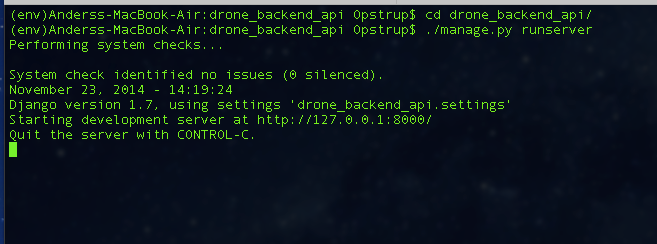
\includegraphics[width=0.85\textwidth]{Billeder/implementation/server_startup.png}
	\caption{Server startup msg}
	\label{fig:server_startup}
\end{figure}
\newpage

\subsubsection*{Mappestruktur}
Dette underafsnit vil forklare om den overordnede mappestruktur i projektet og giver en overordnet forståelse af django udvikling. \\

På figur \ref{fig:mappestruktur_1} ses den overordnet mappestruktur. I roden af mappen findes to væsentlige filer: db.sqlite3 hvilket er database filen til serveren, denne fil vil aldrig blive brugt direkte, men kun indirekte igennem django-frameworket. Den anden fil er manage.py, denne fil er main filen i hele projektet. Filen redigeres aldrig, men bruges kun via terminalen, til forskellige kommandoer på django-applikationen. \\

I roden findes der også to mapper "backend\_api" og "drone\_backend\_api". "drone\_backend\_api"  mappen er selve projekt mappen og "backend\_api" er applikations mappen.

\begin{figure}[H]
	\centering
	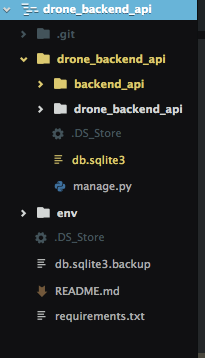
\includegraphics[width=0.2\textwidth]{Billeder/implementation/mappestruktur_1.png}
	\caption{Mappestruktur rod}
	\label{fig:mappestruktur_1}
\end{figure}

På figur \ref{fig:mappestruktur_2} ses projekt mappen, de væsentlige filer i denne mappe er settings.py og urls.py.
Settings.py er filen hvor alle tredje parts applikationer registeres i "INSTALLED\_APPS", filens sikkerhedsindstillinger  sættes op i "MIDDLEWARE\_CLASSES". 
Urls.py filen bruges til at registrere hvilke url's serveren kender og hvilke funktioner og views der skal præsenteres. Yderligere dokumentation omkring settings.py og urls.py kan findes under djangos egen dokumentation omkring settings\footnote{https://docs.djangoproject.com/en/dev/ref/settings/} og urls\footnote{https://docs.djangoproject.com/en/dev/ref/urls/}.

\begin{figure}[H]
	\centering
	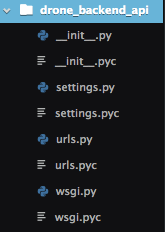
\includegraphics[width=0.2\textwidth]{Billeder/implementation/mappestruktur_2.png}
	\caption{Mappestruktur projekt mappe}
	\label{fig:mappestruktur_2}
\end{figure}

\newpage

På figur \ref{fig:mappestruktur_3} ses applikations mappen. Denne mappe indeholder alt logikken til serveren.

\begin{figure}[H]
	\centering
	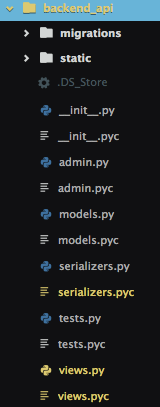
\includegraphics[width=0.2\textwidth]{Billeder/implementation/mappestruktur_3.png}
	\caption{Mappestruktur applikations mappe}
	\label{fig:mappestruktur_3}
\end{figure}

\textbf{admin.py} \\
Denne fil indeholder registrering af diverse tables i projektet. De kan tilgås via en admin page, hvor en administrator kan redigere i det data der ligger i databasen. Yderligere dokumentation omkring admin.py kan findes på\footnote{https://docs.djangoproject.com/en/dev/ref/contrib/admin/}.

\textbf{models.py} \\
Denne fil indeholder alt logikken til hvilke tabeller og attributter der eksistere i databasen. Via denne fil bliver db.sqlite3 filen som findes i roden, manipuleret. Yderligere dokumentation omkring models.py kan findes på\footnote{https://docs.djangoproject.com/en/dev/topics/db/models/}.

\textbf{serializers.py} \\
Denne fil indeholder serializers kaldes når et api-endpoint bliver kaldt. Via disse serializers finder serveren ud af hvilke data der skal hentes fra databasen og repræsenteres. Disse serializers bliver hovedsageligt brugt til at formatere dataen fra databasen til et JSON format. Yderligere dokumentation omkring serializers.py kan findes på\footnote{https://docs.djangoproject.com/en/dev/topics/serialization/}.

\textbf{views.py} \\
Denne fil håndtere de requests som kaldes og afgør ud fra dem hvilke serializer der skal generes og præsenteres. Yderligere dokumentation omkring views.py kan findes på\footnote{https://docs.djangoproject.com/en/dev/topics/class-based-views/}.
\newpage

\subsubsection*{Debug}
Dette underafsnit vil beskrive hvordan server software kan debugges og hvordan de forskellige værktøjer kan bruges.\\

\textbf{Terminal}\\
På figur \ref{fig:get_eksempel} ses et udklip af terminal vinduet, hvor to GET requests har fundet sted. Som det ses på billedet, er det muligt at debugge serveren og tjekke hvilke data sendes frem og tilbage ved hvert request. 

\begin{figure}[H]
	\centering
	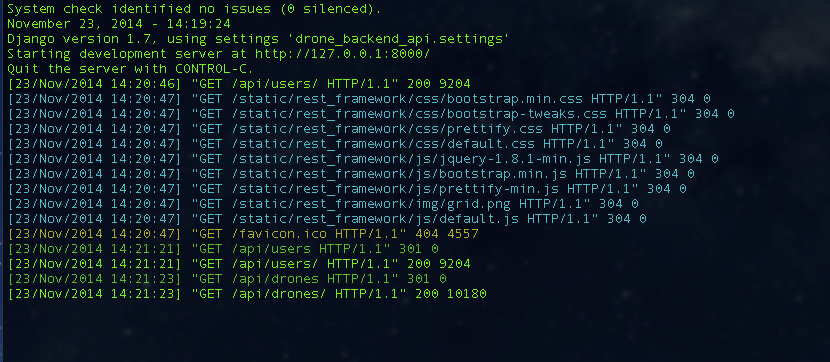
\includegraphics[width=1\textwidth]{Billeder/implementation/get_eksempel.png}
	\caption{GET eksempel}
	\label{fig:get_eksempel}
\end{figure}

\textbf{Browser}\\
På figur \ref{fig:browser_eksempel} ses et andet eksempel på hvordan browseren kan bruges til at debugge serveren. Her ses det hvilke data der kan hentes ved at gå til api-endpoint\\
"http://127.0.0.1:8000/api/drones/". Yderligere information kan findes under Data View afsnittet.

\begin{figure}[H]
	\centering
	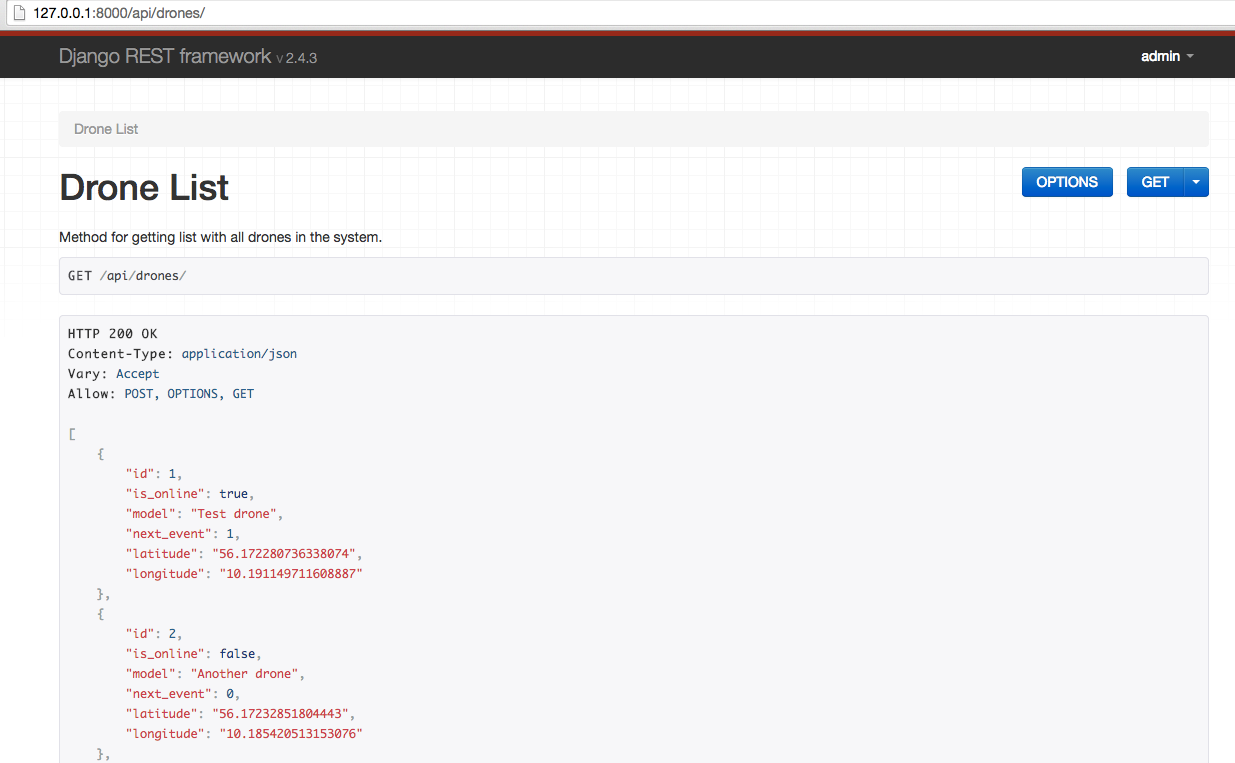
\includegraphics[width=1\textwidth]{Billeder/implementation/browser_eksempel.png}
	\caption{Browser eksempel}
	\label{fig:browser_eksempel}
\end{figure}

\vspace{1cm}

\subsubsection*{Tredje parts teknologier}
Til udviklingen af server softwaren er der benyttet nogle tredje parts teknologier, dette underafsnit beskriver hvilke og hvordan de er blevet brugt.

\textbf{Djangorestframework}\\
Django frameworket er et godt framework til udvikling af webapplikationer.Til projektet ønskes et RESTful api oven på django frameworket, derfor er der brugt et django-rest-frameworket\footnote{http://www.django-rest-framework.org/}. 

\textbf{django-cors-headers}\\
Cors headers\footnote{https://github.com/ottoyiu/django-cors-headers} er et django applikation som tilføjer CORS (Cross-Origin Resource Sharing) til applikationer. Dette gør det muligt at tilgå applikationen fra andre servere, som fx.  client softwaren som kan ligge på en anden server eller dronen som tilgår serveren udefra. 

\newpage

\newpage
\subsection{Opsætning webapplikation udvikling}
Dette afsnit har til formål at beskrive hvordan et udviklingsmiljø sættes op på en givet maskine så vider udvikling af systemet kan finde sted. Afsnittet forklare også hvilke tredjeparts teknologier der er anvendt og eventuelle afhængigheder.

For at kunne opsætte et udviklings miljø til client applikationen skal source koden først hente. Dette kan ske via git, skriv følgende kommando i terminalen.

\begin{lstlisting}[language=bash]
	$ git clone https://github.com/Opstrup/drone_frontend
\end{lstlisting}

\subsubsection*{Mappestruktur}
Dette underafsnit vil forklare om den overordnede mappe struktur i projektet og give en overordnet forståelse af angular client udvikling. \\

På figur \ref{fig:mappestruktur_client} ses mappestrukturen for client applikationen. Da Angular frameworket er opbygget over MVC\footnote{MVC model i forbindelse med Angular: https://docs.angularjs.org/guide/databinding} modellen er mappestrukturen opdelt så det afspejler denne model. I roden af projekt mappen findes to væsentlige file, app.js og index.html. app.js er settings filen for projektet, her bliver alle afhængigheder af projektet hentet ind og initialiseret, states i applikationen og dertilhørende controller bliver også registeret her\footnote{Information omkring app.js indstillingerne: https://docs.angularjs.org/guide/introduction}.\\
index.html er som kendt fra webudvikling den side som bliver hentet først ved et request, da Angular applikationer er et one paged app fungere det lidt specielt. Ved besøg af siden vil index side blive loaded samt javascript- og css-filer. Via Angular frameworket bliver alle andre sider så loaded ind i index siden, hvilket gøre applikationen meget hurtigt da filerne ikke skal indlæses igen.

\begin{figure}[H]
	\centering
	\includegraphics[width=0.2\textwidth]{Billeder/implementation/mappestruktur_client.png}
	\caption{Mappestruktur rod}
	\label{fig:mappestruktur_client}
\end{figure}

\textbf{bower\_components}\\
I denne mappe findes alle treide parts afhængigheder, i form af css og java script filer. Til håndtering af treide parts teknologier er der benyttet bower\footnote{http://bower.io/}, som er et package manager program til webudvikling.

\textbf{controllers}\\
I denne mappe findes alle controller\footnote{https://docs.angularjs.org/guide/controller} i systemet, som fungere på samme måde som kendt fra normal MVC.

\textbf{costum\_css}\\
Ud over bootstrap til håndtering af css'en, er der også blevet lavet nogle små filer med css kode. Disse filer findes i denne mappe.

\textbf{services}\\
I denne mappe findes alle services\footnote{https://docs.angularjs.org/guide/services} i systemet. Disse services indeholder alt buisness logikken i systemet og derved fungere som models i MVC modellen.

\textbf{templates}\\
I denne mappe findes alle html filerne for systemet, disser filer danner sammen med controllerne de views som bliver præsenteret i browseren\footnote{https://docs.angularjs.org/guide/templates}.

\subsubsection*{Udviklings miljø}
Opsætning af et udviklings miljø til client applikationen er rimelig simpel da source koden indeholder alt hvad der skal bruges for at kunne compile, der skal kun bruges en browser for at kunne starte applikationen. Til vider udvikling af applikationen vil det dog anbefales at der installeres nogle applikationer for at gøre udviklingen nemmere.

\textbf{Text editor}\\
Som alt andet web udvikling er det hele scripts som bliver kørt af browseren, derfor er der ingen specielle krav til et IDE af webudvikling. Nogle gode eksempler af text editor til web udvikling ville være Sublime eller Atom\footnote{Yderligere beskrevet i afsnittet om Server Opsætning}.

\textbf{Lokal web server}\\
For at applikationen fungere optimalt er det at anbefale at der installeres en web server på udviklerens maskine. Der er ikke nogle specielle krav til hvilke slags server. En simpel server kunne være en Apache server og for nem installation og opsætning kunne XAMPP\footnote{https://www.apachefriends.org/index.html} benyttes. Et andet eksempel på en web server kunne være en node.js server\footnote{http://nodejs.org/}. 

\textbf{Package management}\\
Som før nævnt er bower brugt til package management og det anbefales at der fortættes med dette da bower\footnote{http://bower.io/} selv downloader og installere de påkrævet filer, så udvikleren ikke skal tænke yderligere over dette.  

\newpage

\subsubsection*{Treide part teknologier}
Til udviklingen af web applikationen er der blevet brugt nogle treide parts teknologier, som er beskrevet yderligere i dette underafsnit.

\textbf{bootstrap}\\
Det populære bootstrap\footnote{http://getbootstrap.com/} css framework er benyttet til at give applikationen et flot design.

\textbf{ui-router}\\
Ui router\footnote{https://github.com/angular-ui/ui-router} er en applikation som er lavet til Angular frameworket som gør routing imellem div views meget simpel. 

\textbf{google-maps}\\
Google maps er blevet brugt til at vise kortet i applikationen og via google maps bliver der også hentet GPS-koordinater til de waypoints som dronen flyver efter. Google maps er ikke blevet benyttet som standart, men et angular applikation\footnote{https://angular-ui.github.io/angular-google-maps/} er blevet benyttet for at fungere bedre med den resterende kode.

\newpage
\section{Timer opsætning}

Da dronen skal flyve autonomt er det påkrævet at dronen skal styres via main controlleren (arduino boardet). Main controlleren styrer dronen ved at sende 6 forskellige pwm signaler til flight control boardet. De 6 pwm signaler bruges til at kontrollere og regulerer henholdsvis: Throttle, yaw, pitch, roll, alttitudehold og flightmode.

For at undgå at lave busywait når de forskellige pwm signaler skal ændres (skift i periodetid eller duty cycle) benyttes tre 16-bit timere som befinder sig på main controlleren. Arduino 2560 boardet har fire forskellige 16-bit timere, som hver kan styre pwm signal (output signal) på to digitale pins, hvis de  bruges korrekt. 

Fordelen ved at bruge timere til at kontrollere de 6 pwm signaler er primært, at pwm signalerne uafhængig og lynhurtigt kan ændres. For at ændre periodetid eller duty cycle på et pwm signal, skal værdien af et eller flere register blot skiftes. 

PWM signalets periodetiden kan forandres ved at ændre værdien af registeret der bruges til at bestemme hvor højt timeren skal ”tælle”, dette register kaldes typisk TOP eller ICRn. 
PWM signalets duty cycle kan forandres ved at ændre værdien af det register der bestemmer hvornår pwm signalet toggles. Dette register kaldes som regel \textit{Output compare}.

Det blev besluttet at bruge følgende tre timere i Fast PWM mode: \\
Timer1 - til kontrol af de to digitale pins 11 og 12.\\
Timer3 -  til kontrol af de to digitale pins 2 og 5.\\
Timer4 - til kontrol af de to digitale pins 6 og 7. \\

Figur \ref{fig:Timing_diagram} viser hvordan output kan se ud ved brug af en timer i Fast PWM mode.  

%kommentar
\begin{figure}[H]
	\centering
	\includegraphics[width=1.\textwidth]{Billeder/Timer/0_timing_diagram.png}
	\caption{Fast PWM Mode, Timing Diagram}
	\label{fig:Timing_diagram}
\end{figure}

\newpage

I det følgende forklares hvordan de tre 16-bit timere er sat op. Bla. forklares valg at mode, udregning af frekvens, samt udregning af hvilke værdier der skal bruges i registerne ICRn og Output compare.

\subsection*{Mode 16-bit timer}

Når main controllerens 16-bits timere benyttes er det muligt at sætte timerne i 16 forskellige modes. Valget af mode styrer dels opløsningen af timeren, men styrer også hvordan timeren skal fungere. Timerne kan bruges i Normal mode, i CTC (Clear Timer on Compare), i Phase Correct PWM Mode eller i Fast PWM.

For at få den størst mulige opløsning benyttes de tre timerne i mode 14 - ”Fast PWM”. I mode 14 bestemmes værdien af TOP, af registeret ICRn som er et 16-bit stort register. Dette betyder at ICRn maksimalt kan sættes til værdien 0xFFFF (65535). 

%kommentar
\begin{figure}[H]
	\centering
	\includegraphics[width=1.\textwidth]{Billeder/Timer/1_mode.png}
	\caption{Fast PWM Mode, Timing Diagram}
	\label{fig:Timing_diagram}
\end{figure}

\newpage

\subsection*{Compare Output Mode}
Når det overordnede mode er valgt for timerne, skal compare output mode vælges. Compare output mode bestemmer hvornår PMW signalet på de forskellige pin sættes helholdvis højt og lavt.

Det besluttes at sætte Compare output mode til:  COMnA1 = 1 og COMnA0 = 0.  Med denne indstilling sættes PWM signalet lavt når timerens counter er lig OCnA eller OCnB og sættes højt igen hver gang timerens counter er lig 0. Indstillingerne sættes på samme vis for COMnB og COMnC.

%kommentar
\begin{figure}[H]
	\centering
	\includegraphics[width=1.\textwidth]{Billeder/Timer/2_compare_output_mode.png}
	\caption{Fast PWM Mode, Timing Diagram}
	\label{fig:Timing_diagram}
\end{figure}

 

\subsection*{TCCR3A}
Da både mode til 16-bit timeren og compare output er valgt kan registeret TCCR3A indstilles. Fra indstilling af mode til 16-bit timeren vides det at WGMn1 = 1, mens WGMn0 = 0. Yderlige vides det at COMnA1 = 1 og COMnA0 = 0 og at COMnB og COMnC skal se ligeledes ud.

Binært skal TCCR3A registeret se således ud: 0b10101010, hvilket i hex svarer til: 0xAA. 

Bemærk: Dette delafsnit tager udgangspunkt i TCCR3A registeret tilhørende timer 3.  TCCR1A og TCCR4A indstilles på samme vis.

%kommentar
\begin{figure}[H]
	\centering
	\includegraphics[width=1.\textwidth]{Billeder/Timer/3_TCCT3A.png}
	\caption{Fast PWM Mode, Timing Diagram}
	\label{fig:Timing_diagram}
\end{figure}

\newpage

\subsection*{Clock select}
Hvilken prescale der vælges har betydning for hvor hurtig en clock der bruges til timeren. I udgangspunkt er det en 16MHz clock der bruges, men ved at bruge prescale er det muligt at mindske clocken. Når der gøres brug af en 16-bit timer, har counteren maksimalt 65535 steps. 

Ud fra viden om clockens hastighed og antal steps i counteren kan frekvensen på timernes PWM signal udregnes således: Clock / antal steps = 244,14 Hz.  

Hvilket giver følgende periodetid: 1 / 244,14 Hz = 4,096 ms.

Sættes der prescale på clock’en vil frekvensen falde og periodetiden stige. Men da der ønskes periodetid så tæt på 2ms vælges det ikke at bruge prescale. 

%kommentar
\begin{figure}[H]
	\centering
	\includegraphics[width=1.\textwidth]{Billeder/Timer/4_CS.png}
	\caption{Fast PWM Mode, Timing Diagram}
	\label{fig:Timing_diagram}
\end{figure}
  

\subsection*{TCCR3B}
Da både mode til 16-bit timeren og clock select er valgt kan registeret TCCR3B indstilles. Fra indstilling af mode til 16-bit timeren vides det at WGMn3 = 1, mens WGMn2 = 1. Yderlige vides det at CSn2 = 0, CSn1 =0 og CSn0 = 1. 

Både ICNC3 (Input Capture Nolse Canceler) og ICES3 (Input Capture Edge Select) sættes lig 0.
Binært skal TCCR3B registeret se således ud: 0b00011001, hvilket i hex svarer til: 0x19. 

Bemærk: Dette delafsnit tager udgangspunkt i TCCR3B registeret tilhørende timer 3.  Registrene TCCR1B og TCCR4B tilhørende timer 1 og 4 indstilles på samme vis.

%kommentar
\begin{figure}[H]
	\centering
	\includegraphics[width=1.\textwidth]{Billeder/Timer/5_TCCT3B.png}
	\caption{Fast PWM Mode, Timing Diagram}
	\label{fig:Timing_diagram}
\end{figure}


\subsection*{TCCR3C}
Force Output Compare A, B og C bruges kun når timeren er sat til et ikke PWM mode.  Derfor sættes Force Output Compare A, B og C = 0.
Binært skal TCCR3B registeret se således ud: 0b00000000, hvilket i hex svarer til: 0x00. 

Bemærk: Dette delafsnit tager udgangspunkt i TCCR3C registeret tilhørende timer 3.  Registrene TCCR1C og TCCR4C tilhørende timer 1 og 4 indstilles på samme vis.

%kommentar
\begin{figure}[H]
	\centering
	\includegraphics[width=1.\textwidth]{Billeder/Timer/6_TCCT3C.png}
	\caption{Fast PWM Mode, Timing Diagram}
	\label{fig:Timing_diagram}
\end{figure}
 

\subsection*{Indstilling Top og Compare match}
Reelt set er opsætningen af duty cycle og periodetid fuldstændig ligegyldigt. Det eneste der betyder noget, er at de PWM signaler der sendes til flight control boardet har pulsbredde mellem 1-2 ms.
 
Det vides at periodetiden på pwm signalerne vil være 4,096 ms når der arbejdes med clock på 16MHz, der ikke benyttes prescale og Top = 65535.

Ved opstilling af to simple ligninger, kan det beregnes hvilken værdi der skal skrives ind i compare match registeret for at skabe et pwm signal med pulsbredde på 1 ms.  

4,096 ms * x = 1 ms	Udtrykket omformes til: 	x = 1 ms / 4,096 ms = 0,244.

Værdi af Compare match for at opnå pulsbredde på 1ms:  Top * x = 65535 * 0,244 ~ 16000.

På samme vis kan det udregnes hvilken værdi der skal skrives i compare match for at få pulsbredde på 2 ms.

4,096 ms * x = 2 ms	Udtrykket omformes til: 	x = 2 ms / 4,096 ms = 0,488

Værdi af Compare match for at opnå pulsbredde på 1ms:  Top * x = 65535 * 0,488 ~ 32000.

Det er nu beregnet: Pulsbredde på 1ms fås ved compare match = 16000, mens pulsbredde på 2ms fås ved compare match = 32000. For at styre flight control board skal værdien i compare match altså veksle op og ned i størrelse mellem 16000 og 32000. 









